\chapter{Imperative und deklarative Modellierung für SE-Prozessmodelle}\label{sec:chapter6}
In diesem Kapitel wird der Vergleich zwischen imperativer und deklarativer Modellierung für SE-Prozessmodelle gezogen. Als Erstes wird dieser Vergleich in Kapitel 6.1 für das SE-Prozessmodell Scrum durchgeführt. Hierfür wird zunächst in Kapitel 6.1 das der Modellierung zugrunde liegende Modell, das SE-Prozessmodell Scrum, vorgestellt und in Kapitel 6.1.1 für die Modellierung analysiert. Danach erfolgt in Kapitel 6.1.2 die imperative Modellierung in der Prozessmodellierungssprache BPMN und anschließend die deklarative Modellierung in der Prozessmodellierungssprache ConDec in Kapitel 6.1.3. Danach erfolgt  in Kapitel 6.1.4 der Vergleich zwischen den beiden Modellen.\newline
Der zweite SE-Prozess, welcher in diesem Kapitel in imperativer und deklarativer Prozessmodellierungssprache verglichen werden soll, ist der Open Unified Process (Open Up). Auch hier erfolgt zunächst eine kurze Einführung in den Open Up in Kapitel 6.2, bevor dieser in Kapitel 6.2.1 analysiert wird, damit er in den Kapiteln 6.2.2 und 6.2.3 in imperativer, bzw. deklarativer Prozessmodellierungssprache modelliert werden kann. Hiernach erfolgt in Kapitel 6.2.4 der Vergleich zwischen den Prozessmodellen.\newline
Zuletzt werden noch für das V-Modell XT die Prozessmodelle erstellt und verglichen. Eine Einführung in das V-Modell XT erfolgt in Kapitel 6.3. In Kapitel 6.3.1 wird für dieses als Vorbereitung für die Modellierung eine Analyse durchgeführt und in den Kapiteln 6.3.2 und 6.3.3 erfolgt die Modellierung in imperativer und deklarativer Prozessmodellierungssprache. Der Vergleich hierzu erfolgt in Kapitel 6.3.4.


\section{Scrum}\label{sec:chapter6:Imperative Modellierung}

Der Begriff Scrum stammt aus dem Artikel "The New New Product Development Game", welchen Hirotaka Takeuchi und Ikujiro Nonaka im Harvard Business Review 1986 veröffentlicht haben. Sie beschrieben einen ganzheitlichen Ansatz, bei dem kleine, funktionsübergreifende Teams zusammen an einem gemeinsamen Ziel arbeiten. Dies verglichen sie mit der Scrum-Formation beim Rugby \cite{Pham2012,Takeuchi1986}. \newline
Bei Scrum handelt es sich um ein agiles Prozessmodell, welches seit Anfang 1990 für komplexe Entwicklungen verwendet wird. Agile Prozessmodelle werden den leichtgewichtigen Prozessmodellen zugeordnet \cite{Hanser2010, Lacey2012}. Einen ersten Überblick über das Scrum-Prozessmodell gibt Abbildung \ref{fig:Scrum}:

\begin{figure}[htp]
\begin{center}
  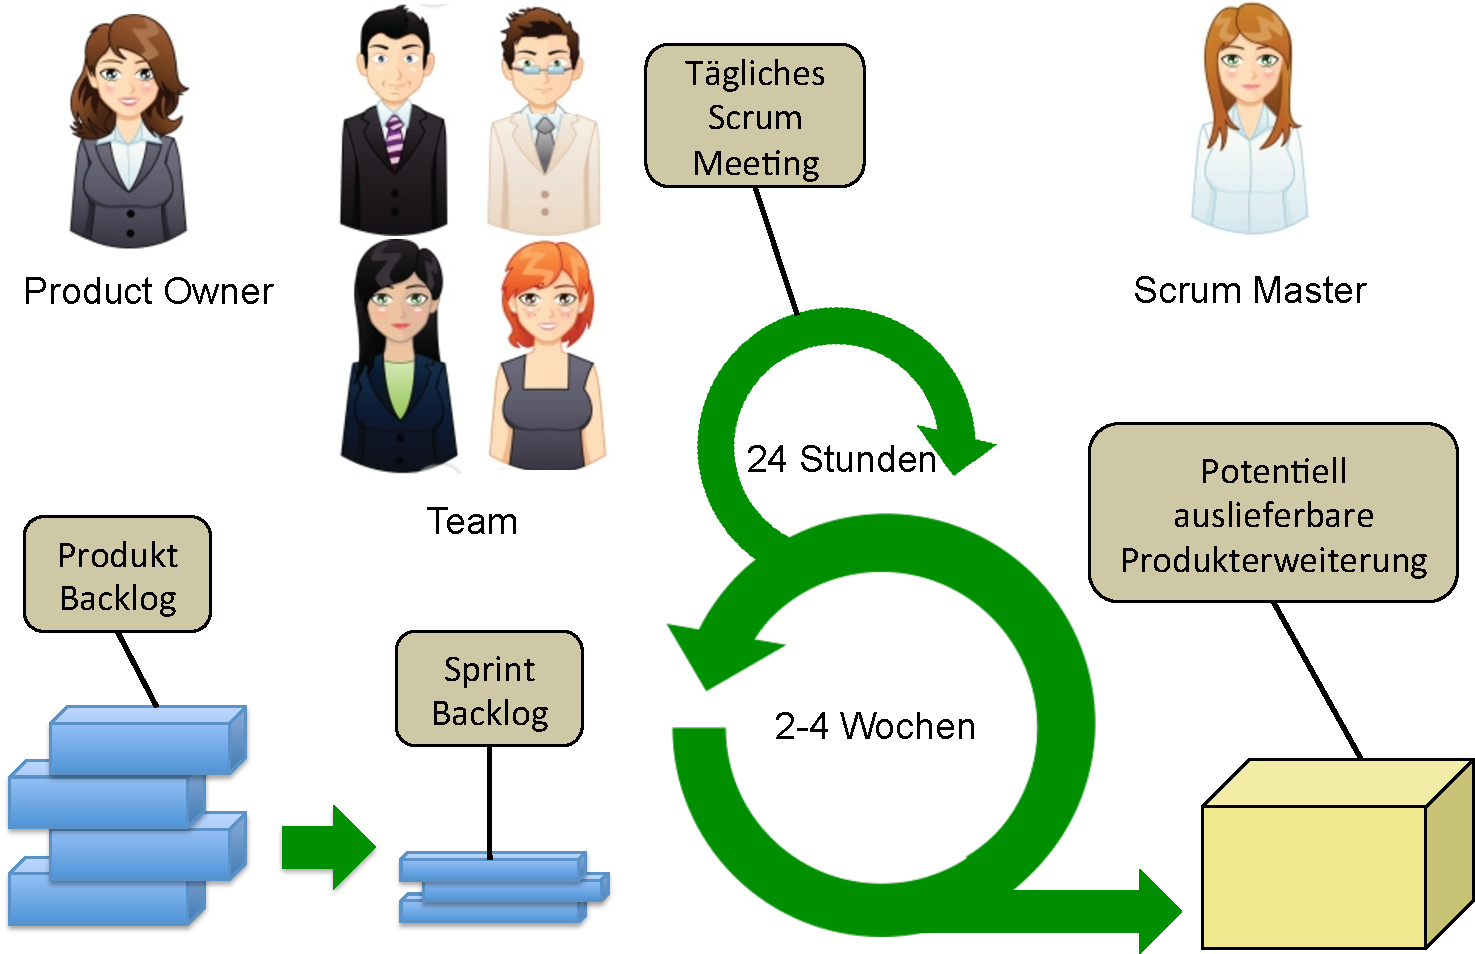
\includegraphics[scale=0.6]{Scrum} %pdf, jpg, png...
  \caption{Scrum Überblick nach \cite{scrum2008}}
  \label{fig:Scrum}
\end{center}
\end{figure}

Der genaue Ablauf im Scrum Prozessmodell wird nachfolgend genau analysiert.

\subsection{Analyse Scrum}


Im Scrum-Prozessmodell gibt es nur drei verschiedene Rollen: Den \textit{Product Owner}, das \textit{Team} und den \textit{Scrum Master}. Sämtliche Verantwortlichkeiten innerhalb eines Projektes werden hierbei auf diese drei Rollen aufgeteilt \cite{Schwaber2004}. \newline

Der \textit{Procuct Owner} ist verantwortlich, die Interessen aller am Projekt beteiligten Personen zu vertreten. Neben der Budgetierung des Projektes erstellt er ebenfalls Releasepläne und erstellt den Produkt-Backlog, welcher eine Liste mit funktionalen und nicht-funktionalen Anforderungen darstellt \cite{Schwaber2004, Pichler2010,Schwaber2007}. Weiterhin priorisiert er die Aufgaben, welche von den Entwicklern im Sprint erledigt werden sollen, so dass die aktuell nützlichsten Elemente die höchste Priorität haben. Er erstellt eine Liste dieser Elemente, welche \textit{Sprint-Backlog} genannt wird \cite{Henning2011, Schwaber2007,Pichler2010}. Der \textit{Procuct Owner} ist ebenfalls zuständig für das Annehmen, bzw. Ablehnen der Arbeitsergebnisse \cite{eclipseScrum}. \newline

Die \textit{Teams} bestehen bei Scrum für gewöhnlich aus fünf bis neun Mitgliedern und verwalten sich selbst. Ihre Tätigkeiten müssen erfolgreich sein, liegen aber in ihrer eigenen Verantwortung \cite{Pries2011, Wolf2011}. Alle Teammitglieder sind gemeinsam für den Erfolg eines jeden \textit{Sprints} und des gesamten Projektes verantwortlich \cite{Pichler2010}. \newline

Der \textit{Scrum-Master} ist für den gesamten Scrum-Prozess verantwortlich. Dies schließt die Vermittlung von Scrum-Inhalten (z.B. Schulungen) und die Implementation von Scrum in die Unternehmenskultur ein \cite{Pichler2010}. Er überwacht die Sprint- Tasks, um sicher zu gehen, dass der Sprint erfolgreich verläuft.\newline

Bei Scrum wird die Entwicklung in mehrere kurze Zyklen, also Iterationen eingeteilt. Eine einzelne Iteration wird bei Scrum \textit{Sprint} genannt \cite{Henning2011}. Die Dauer eines Sprints beträgt zwei bis vier Wochen. Am Ende eines jeden Sprints muss das \textit{Team} ein lauffähiges Produkt abliefern \cite{Wolf2011}. Vor jedem Sprint findet ein \textit{Sprint Planning Meeting} statt, welches sich aus zwei Teilen zusammensetzt \cite{Pichler2010}. Im ersten Teil findet eine Planung des nächsten \textit{Sprints} statt \cite{Lacey2012}. Hierfür präsentiert der \textit{Product Owner} dem \textit{Team} eine Liste der Product-Backlog-Elemente mit der aktuell höchsten Priorität \cite{Schwaber2004, Schwaber2007,Pichler2010}. Diese Liste wird \textit{Sprint-Backlog} genannt \cite{Wolf2011}. Das \textit{Team} hat die Möglichkeit, Fragen bezüglich Inhalt, Zweck, Bedeutung und Absichten der \textit{Sprint-Backlog}-Elemente zu stellen. Anschließend werden die einzelnen Elemente aus dem \textit{Sprint-Backlog} in sogenannte \textit{Tasks} aufgeteilt, welche jeweils eine ideale Bearbeitungszeit von zwei bis vier Stunden haben, aber niemals länger als zwei Tage dauern sollten \cite{Wolf2011}. Das \textit{Team} kann sich die Aufgaben eigenverantwortlich aufteilen und muss sich anschließend dem \textit{Product  Owner} verpflichten, die \textit{Tasks} bis zum Abschluss des \textit{Sprints} zu erledigen \cite{Wolf2011, Keith2010,Pichler2010}.
Das  \textit{Team} trifft sich während des \textit{Sprints} täglich in einem 15-minütigen Meeting, dem \textit{täglichem Scrum-Meeting}. Dabei redet das \textit{Team} über seinen Fortschritt und eventuelle Probleme bei seiner Arbeit \cite{Keith2010}. Hier muss jedes Teammitglied die nachfolgenden drei Fragen beantworten \cite{Wolf2011}:
   \begin{enumerate}
      \item Was habe ich seit gestern erreicht?
      \item Was werde ich heute erreichen?
      \item Was blockiert mich?
      \end {enumerate}
      
\subsection{Imperative Modellierung Scrum}

Abbildung \ref{fig:ScrumImperativ} zeigt die imperative Modellierung von Scrum. \newline
Im Prozess gibt es die drei verschiedenen Rollen \textit{Product Owner}, \textit{Team} und \textit{Scrum Master}, was im Prozessmodell durch drei verschiedene Swimlanes dargestellt ist, welche die jeweilige Rolle repräsentieren.\newline
Parallel zu allen anderen Aktivitäten des Teams und des Product Owners muss der Scrum-Master stets den Scrum-Prozess managen. Dies wird im Prozessmodell durch das parallele Gateway dargestellt. \newline
Der Product Owner schätzt als erste Aktivität den Product Backlog ab. Anschließend priorisiert er den Product Backlog und erstellt parallel dazu die Releasepläne. \newline
Wenn alle zwei bis vier Wochen ein neuer Sprint beginnt, was hier durch ein Zeitereignis dargestellt ist, so wird zuerst das Sprint Planning Meeting durchgeführt. Dies ist hier als Unterprozess in Abbildung \ref{fig:ScrumImperativUnter} dargestellt. Zunächst priorisiert der Product Owner die Anforderungen, welche während des Sprints erledigt werden müssen und erstellt danach den Sprint Backlog. Anschließend teilt sich dann das Team selbstständig die Sprint Backlog-Elemente in Tasks ein.\newline
Im Anschluß findet ein Sprint-Rückblick statt (Abbildung \ref{fig:ScrumImperativ}) und der Product Owner führt ein Sprint Review Meeting durch.\newline
Das Team führt während des Sprints täglich ein 15-minütiges Scrum Meeting durch und jedes Teammitglied arbeitet eine Task nach der anderen ab. Dies wird hier als Schleife dargestellt: Solange noch weitere Tasks vorhanden sind, führt das Exklusive Gateway immer wieder zurück zur Aktivität \textit{Tasks abarbeiten}. Erst wenn keine weiteren Tasks mehr vorhanden sind, führt der Prozess weiter zum nächsten Entscheidungspunkt.\newline
Sind noch weitere Aufgaben im Product Backlog vorhanden, die noch erledigt werden müssen, so beginnt ein weiterer Sprint, was hier durch eine Rückschleife dargestellt ist. Ist jedoch schon der komplette Product Backlog abgearbeitet, so endet der Prozess hier.


\begin{figure}[htp]
\begin{center}
  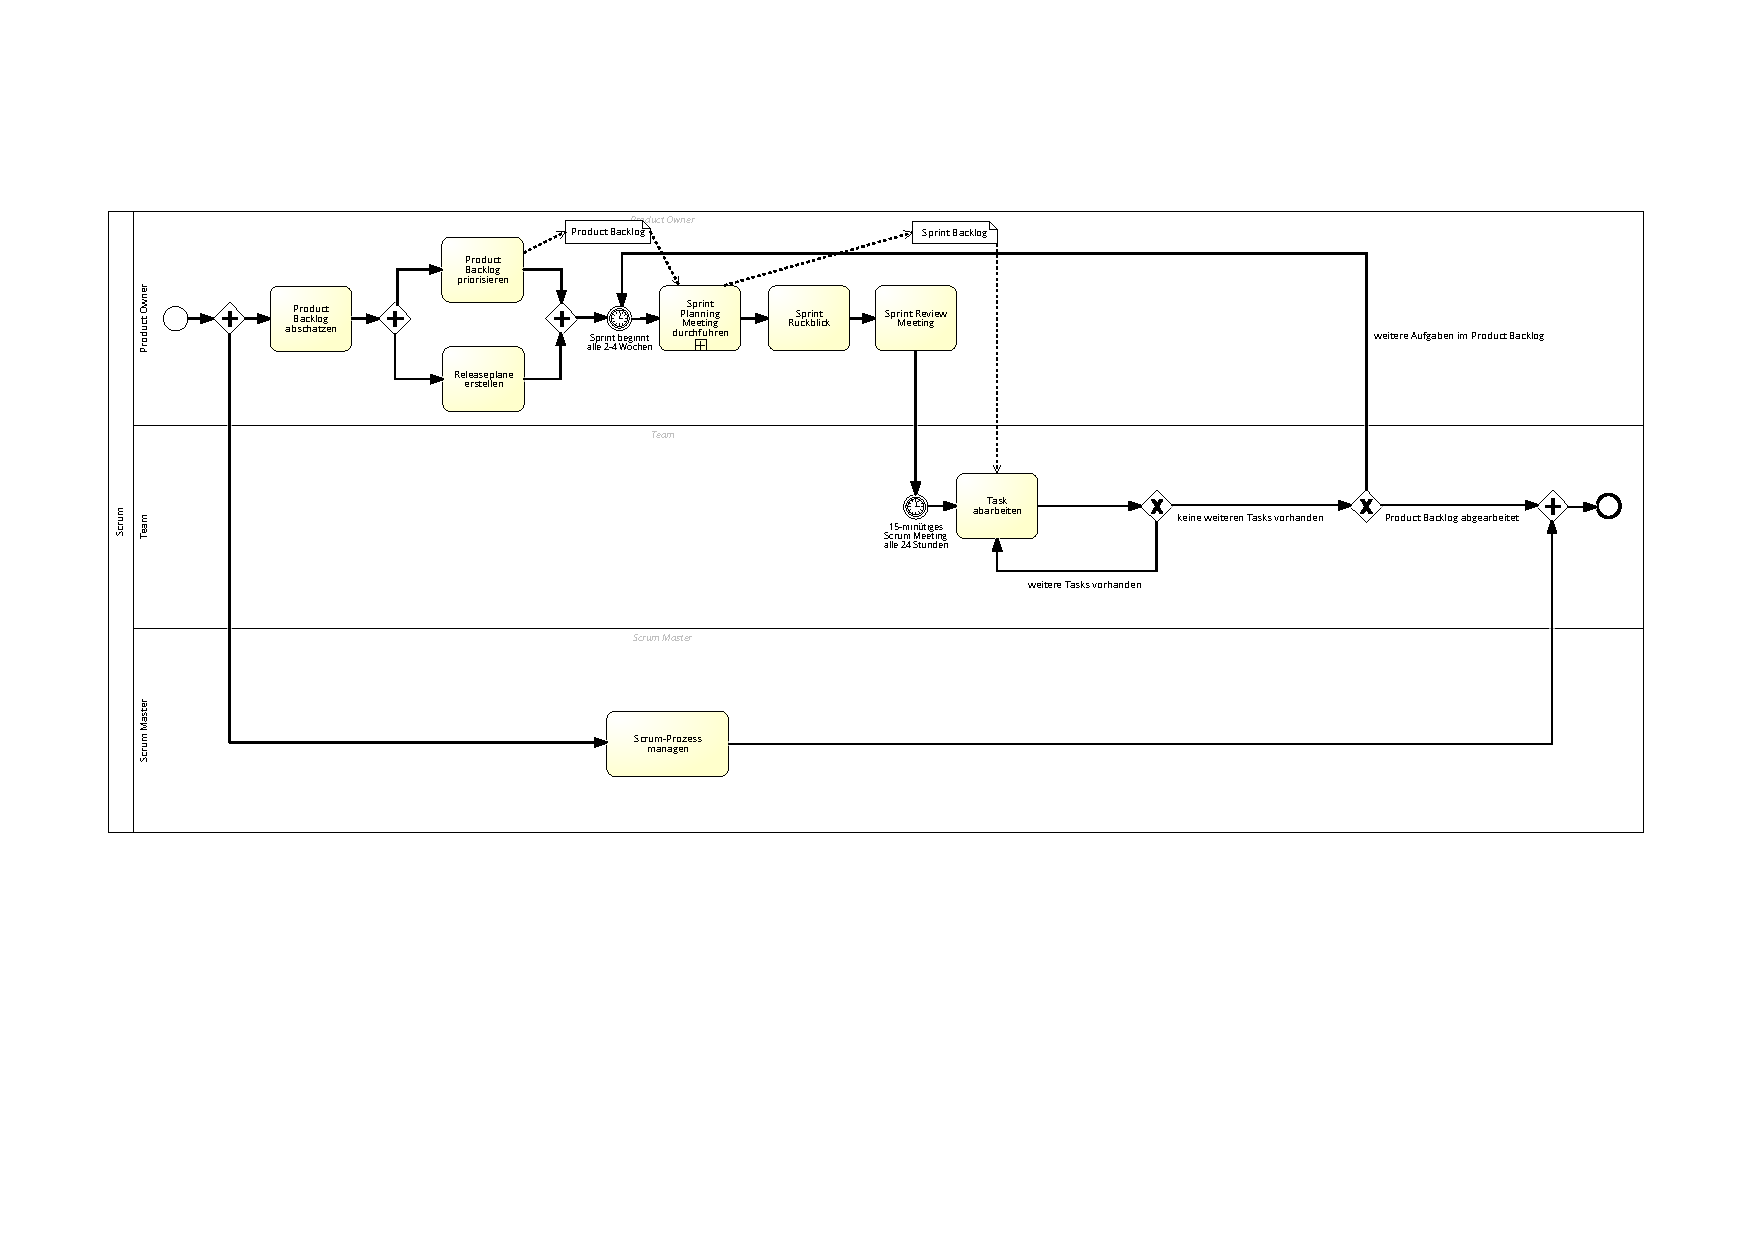
\includegraphics[width=\textwidth]{ScrumImperativ} %pdf, jpg, png...
  \caption{Imperative Modellierung Scrum}
  \label{fig:ScrumImperativ}
\end{center}
\end{figure}

\begin{figure}[htp]
\begin{center}
  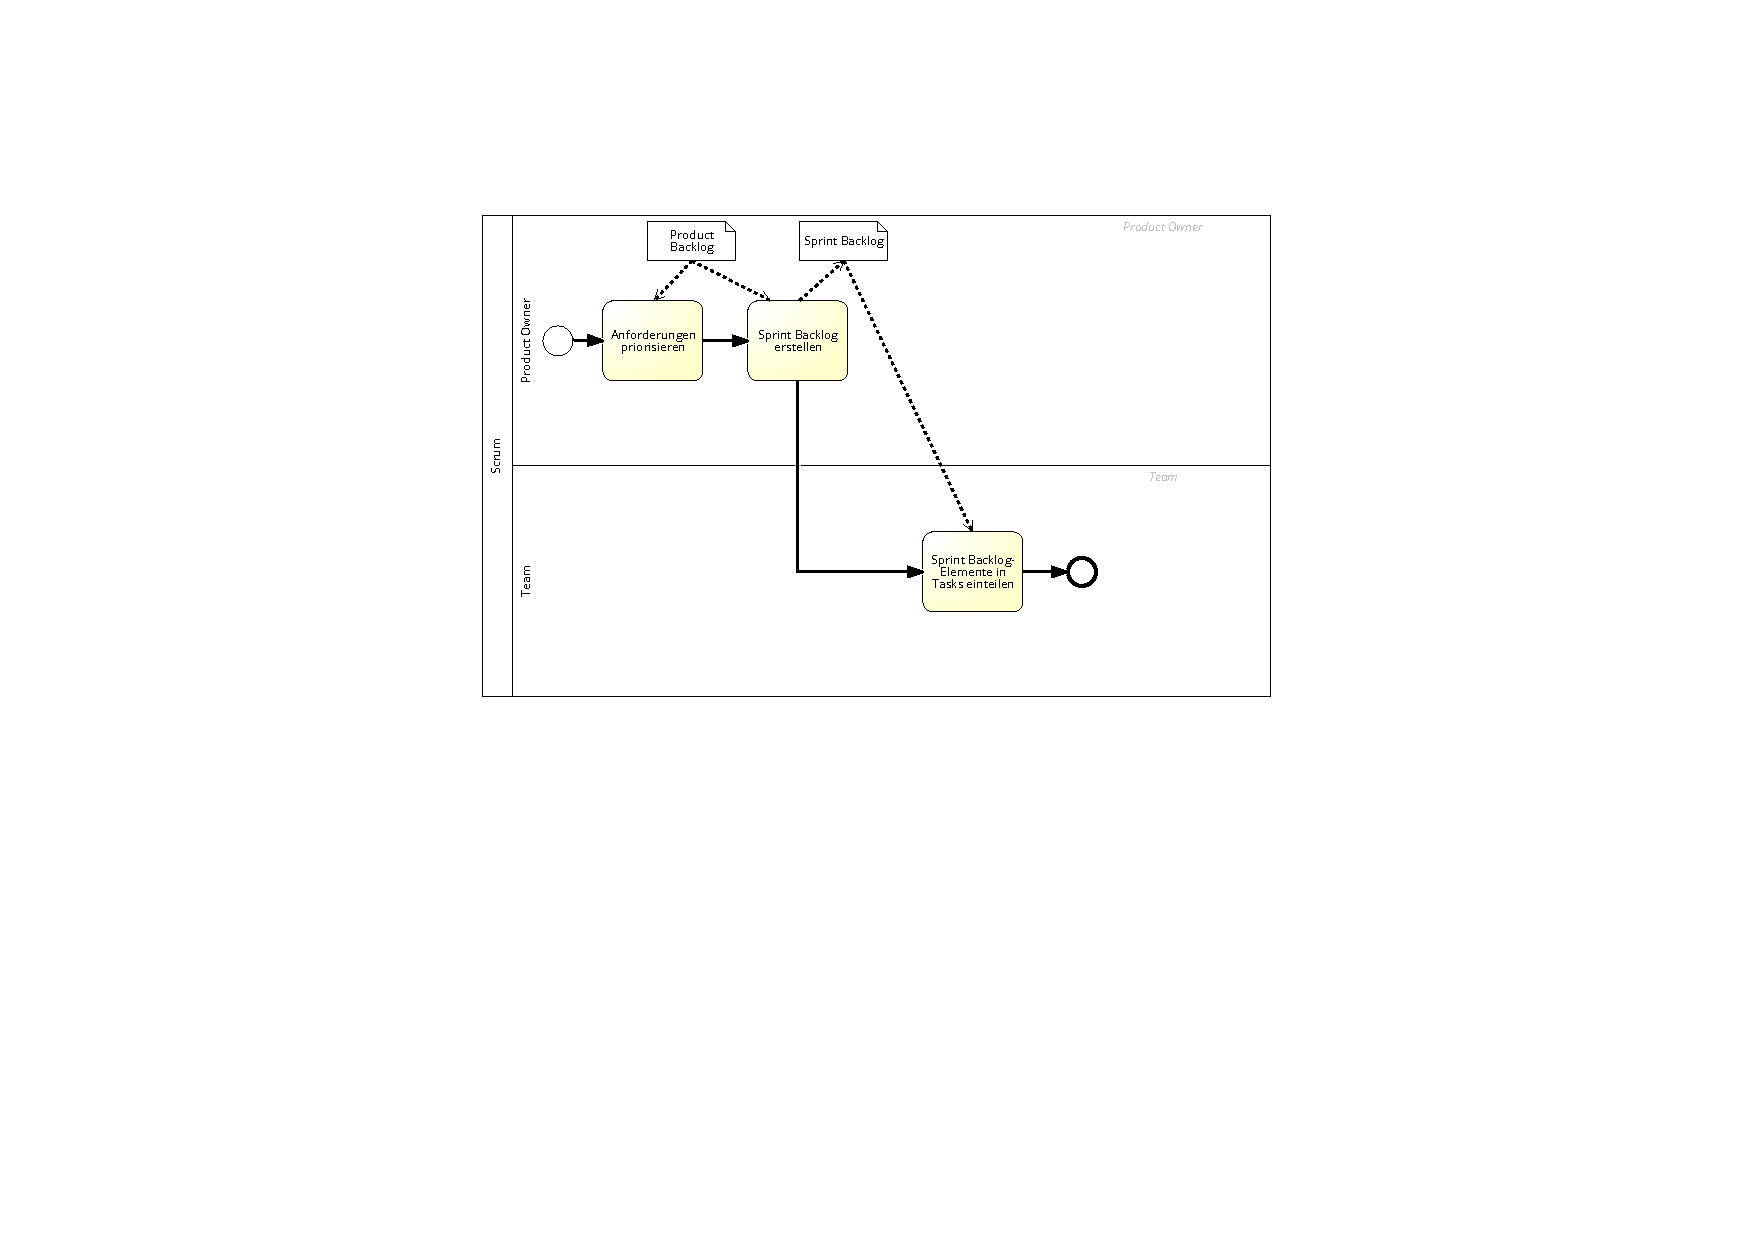
\includegraphics[scale=0.7]{ScrumImperativUnter} %pdf, jpg, png...
  \caption{Imperative Modellierung Scrum Unterprozess}
  \label{fig:ScrumImperativUnter}
\end{center}
\end{figure}
\clearpage

\subsection{Deklarative Modellierung Scrum}

Abbildung \ref{fig:ScrumDecHaupt} zeigt die deklarative Modelliereung von Scrum.\newline
Der Prozess beginnt mit der Aktivität \textit{Product Backlog} abschätzen. Dies ist hier durch das init-Constraint gekennzeichnet. Weiterhin wird diese Aktivität im Prozess genau einmal ausgeführt, was durch das exactly (1)- Constraint dargestellt ist. Das Constraint \textit{succession} gibt an, dass die Aktivität \textit{Product Backlog abschätzen} vor den Aktivitäten \textit{Product Backlog priorisieren} und \textit{Releasepläne erstellen} ausgeführt werden müssen und dass die Aktivitäten \textit{Product Backlog priorisieren} und \textit{Releasepläne erstellen} auf jeden Fall nach \textit{Product Backlog abschätzen} durchgeführt werden müssen. \textit{Product Backlog priorisieren} und \textit{Releasepläne erstellen} werden ebenfalls genau einmal ausgeführt, was durch das exactly (1)- Constraint festgelegt wird.  \newline

Nach deren Ausführung muss die Aktivität \textit{alle 2-4 Wochen Sprint Planning Meeting durchfuehren} erfolgen. Der zugehörige Unterprozess ist in Abbildung \ref{fig:ScrumDecUnterprozess} zu finden. Hier sind die Aktivitäten \textit{Anforderungen priorisieren}, \textit{Sprint Backlog erstellen} und \textit{Sprint-Backlog-Elemente in Tasks einteilen} durch das Constraint \textit{precedence} miteinander verbunden, um die Einhaltung deren Reihenfolge nacheinander zu gewährleisten. Außerdem dürfen diese Aktivitäten pro Ausführung des Unterprozesses, also pro Prozessinstanz nur einmal ausgeführt werden.\newline
Nach der Ausführung der Aktivitäten des Unterprozesses Sprint-Planning-Meeting durchführen, muss im Anschluß die Aktivität \textit{Sprint Rückblick} durchgeführt werden. Dies wird durch das Constraint \textit{chain response} sichergestellt.Eine erneute Ausführung von  \textit{alle 24 Stunden 15-minütiges Scrum-Meeting durchführen} ist erst nach Durchführung von \textit{Sprint Rückblick} möglich (Constraint \textit{alternate precedence}). Hierdurch wird eine Schleife modelliert, welche den immer wiederkehrenden Sprint simuliert.\newline
Die Aktivitäten \textit{alle 24 Stunden 15-minütiges Scrum-Meeting durchführen} und \textit{Tasks abarbeiten} können während des Sprints so oft wie nötig durchgeführt werden. Die Aktivitäten  \textit{alle 24 Stunden 15-minütiges Scrum-Meeting durchführen} und \textit{Tasks abarbeiten} müssen jedoch nebeneinander ausgeführt werden, was durch das Constraint \textit{succession} beschrieben ist. \newline


\begin{figure}[htp]
\begin{center}
  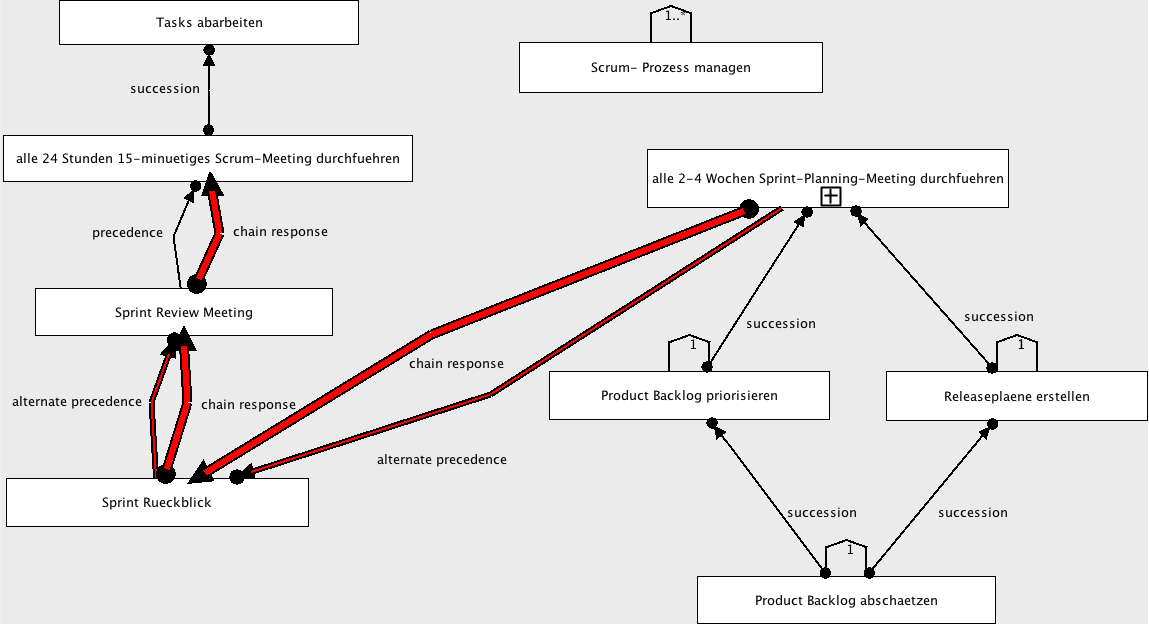
\includegraphics[width=\textwidth]{ScrumDecHaupt} %pdf, jpg, png...
  \caption{Deklarative Modellierung Scrum}
  \label{fig:ScrumDecHaupt}
\end{center}
\end{figure}



\begin{figure}[htp]
\begin{center}
  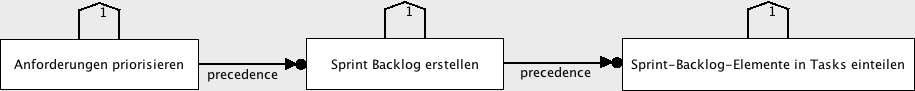
\includegraphics[width=\textwidth]{ScrumDecUnterprozess} %pdf, jpg, png...
  \caption{Deklarative Modellierung Scrum-Unterprozess Sprint-Planning-Meeting durchführen}
  \label{fig:ScrumDecUnterprozess}
\end{center}
\end{figure}
\clearpage

\subsection{Vergleich}

Der Vergleich zwischen den in der deklarativen Prozessmodellierungssprache ConDec und dem in der imperativen Prozessmodellierungssprache BPMN erstellten Scrum Prozessmodellen wird im Folgenden anhand der in Kapitel 5 definierten Anforderungen durchgeführt. \newline
Wie Abbildung \ref{fig:ScrumExcel} entnommen werden kann, unterscheidet sich die Anzahl der Aktivitäten zwischen den in BPMN und ConDec modellierten Prozessmodellen nicht voneinander. In jedem Prozessmodell gibt es 12 Aktivitäten.\newline

\begin{figure}[htp]
\begin{center}
  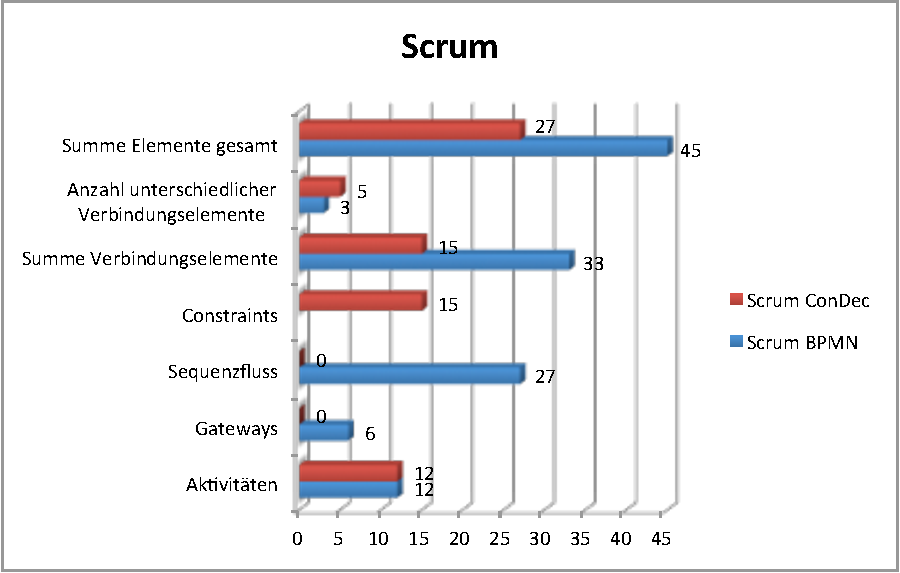
\includegraphics[scale=0.8]{ScrumExcel} %pdf, jpg, png...
  \caption{Vergleich der Anzahl der Elemente Scrum}
  \label{fig:ScrumExcel}
\end{center}
\end{figure}


Zudem braucht es in BPMN sechs Gateways und 26 Sequenzflusselmente, um den Ablauf des Metamodells darzustellen. Bei Verwendung von ConDec werden 13 Constraints für den Ablauf der Aktivitten und sieben Existenz Constraints benötigt. In BPMN werden jedoch nur zwei verschiedene Verbindungselemente verwendet, während es in ConDec vier verschiedene Verbindungselemente sind.\newline

Die \textit{Richtigkeit} lässt sich mit BPMN in Bezug auf Rollen und Artefakte besser einhalten, als mit ConDec. Da es bei ConDec keine Möglichkeit gibt, Rollen und Artefakte im Prozessmodell selbst abzubilden, müssen diese Informationen weggelassen werden. Die Rollen und Artefakte können zwar in Declare abgebildet werden, jedoch ist dies auf Papier/Bild nicht sichtbar. Aus desem Grund müssen diese Informationen beim Modellieren weggelassen werden, was zur Folge hat, dass das im Metamodell beschriebene Verhalten nicht vollständig abgebildet werden kann und somit leidet auch der Nutzen des Modells.\newline

Nur BPMN bietet die Möglchkeit, Artefakte im Prozessmodell abzubilden und lässt somit die Integration anderer Sichten in das Modell zu. Somit kann der Modellierungsgrundsatz des \textit{systematischen Aufbaus} nur von BPMN eingehalten werden. Da ConDec dies nicht zulässt, schmälert es die Eignung von ConDec zum Modellieren in Bezug auf Softwareprozessmodelle. Hierdurch können wichtige Informationen aus dem Metamodell nicht abgebildet werden. \newline 

Beide Prozessmodelle können mit minimal relevanten Informationen erstellt werden. Bei keiner der beiden Modellierungssprachen war es notwendig, weitere Informationen zum Modell hinzuzufügen, um dessen Qualität zu erhöhen. Somit kann \textit{Relevanz} bei beiden Prozessmodellen eingehalten werden.\newline


\textit{Wirtschaftlichkeit} lässt sich mit beiden Modellierungssprachen einhalten. Die Aufwände zum Erstellen der Modelle unterscheiden sich in den beiden verwendeten Sprachen nicht voneinander.\newline

Bei Untersuchung der \textit{Klarheit} lässt sich feststellen, dass sich die Anzahl der Aktivitäten nicht unterscheidet, jedoch die Anzahl der Gateways/Constraints und die Anzahl der unterschiedlichen Gateways/Constraints. Wie in Kapitel 5 bereits erwähnt, kann sich eine größere Anzahl an Gateways/Constraints negativ auf die Verständlichkeit auswirken. Hier ist die Anzahl bei ConDec mehr als doppelt so hoch wie bei BPMN. In BPMN werden insgesamt zwei verschiedene Gateways (ein exklusives Gateway und ein paralleles Gateway) verwendet zur Darstellung von Verzweigungen. In ConDec werden vier verschiedene Constraints zur Darstellung verwendet. Da das Verständnis der Constraints in ConDec an sich relativ schwierig ist, ist das Verständnis eines Prozessmodelles mit vielen verschiedenen Constraints relativ schwer. Da die Anzahl der unterschiedlichen Verbindungselemente hier bei ConDec doppelt so hoch ist wie bei BPMN und es sich bei vier der unterschiedlichen Constraints um sehr komplexe Constraints handelt, ist hier BPMN trotz der höheren Anzahl an Elementen das verständlichere Modell.
\newline

Die \textit{Vergleichbarkeit} in Betracht des Ausführungsverhaltens der beiden Modelle wurde durch Testausführungen in den Modellierungstools Signavio und Declare gewährleistet.\newline
Bei BPMN weist das erstellte Modell insgesamt mehr Elemente auf. Während bei ConDec insgesamt 32 Elemente benötigt werden, werden zur Darstellung des gleichen Sachverhaltes bei BPMN 44 Elemente verwendet. \newline
Bei ConDec müssen Informationen wie Rollen und Artefakte weggelassen werden, während sie in BPMN dargestellt werden können.\newline
Die \textit{Vergleichbarkeit} kann zwar in Bezug auf das Ausführungsverhalten von beiden Sprachen eingehalten werden. BPMN weist jedoch insgesamt mehr Elemente auf und ConDec kann die \textit{Vergleichbarkeit} in Bezug auf die Darstellbarkeit von Rollen und Artefakten nicht einhalten. Somit liegt hier keine der beiden Prozessmodellierungssprachen vorne.\newline

Abbildung \ref{fig:TabelleScrum} zeigt die Ergbenisse des Vergleichs von BPMN und ConDec nochmals in der Zusammenfassung. Somit liegt BPMN bei den Grundsätzen \textit{Richtigkeit}, \textit{systematischer Aufbau}, \textit{Klarheit} und \textit{Vergleichbarkeit} vorne, bei den Grundsätzen \textit{Wirtschaftlichkeit} und \textit{Relevanz} liegen BPMN und ConDec gleich auf. \newline

\begin{figure}[htp]
\begin{center}
  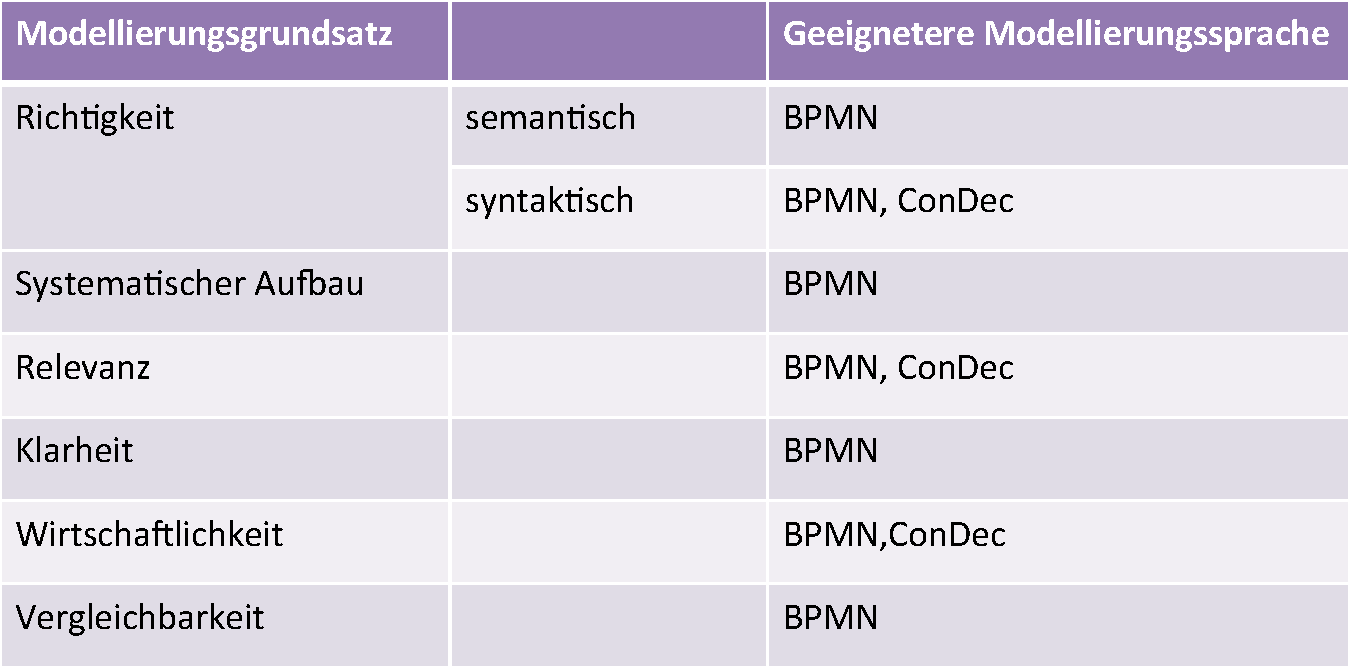
\includegraphics[scale=0.6]{TabelleScrum} %pdf, jpg, png...
  \caption{Zusammenfassung Vergleich Scrum}
  \label{fig:TabelleScrum}
\end{center}
\end{figure}




\section{Open Unified Process (Open UP)}


Der Open Unified Process, kurz Open Up ist eine frei zugängliche Variante des Rational Unified Process, welcher ein sehr bekannter Entwicklungsprozess ist \cite{hauber2010}.  Er ist Teil des Eclipse Process Frameworks. Open Up ist ein iterativer, inkrementeller und minimaler Prozess, aber dennoch vollständig und erweiterbar \cite{Gau2006, Basem2010}. Der Prozess ist minimal gehalten, weil er nur die wesentlichen Inhalte einbezieht. Trotzdem ist er vollständig, da er als Prozess benutzt werden kann, um ein Softwaresystem zu entwickeln. Er ist außerdem auch erweiterbar, da er als Grundlage herangezogen werden kann und mit weiteren Prozessfragmenten aufgestockt und nach Belieben zugeschnitten werden kann \cite{Wang2007}. Das Konzept des Open Up ist es, den Prozess zu vergrößern, sich aber auf das Minimum, welches für das Projekt benötigt wird, zu beschränken, anstatt zu versuchen große, überladene Prozesse zu verstehen und diese dann zu verkleinern \cite{ambler2012}.  \newline



Open Up ist auf kleine Teams ausgerichtet, bei welchen bei der Zusammenarbeit räumliche Nähe besteht. Die Teammitglieder haben hierbei die Freiheit, ihre eigenen Entscheidungen bezüglich ihren aktuellen Aufgaben und Prioritäten zu treffen, um die Anforderungen der Stakeholder zu erfüllen. Das Team trifft sich täglich, um über den aktuellen Status zu reden \cite{OpenUPProcess}.\newline
Es werden Rollen, Aufgaben, Artefakte und Ebenen in Open Up definiert. Dies soll ermöglichen, dass verschiedene Sichten, die sich in ihrem Detaillierungsgrad unterscheiden auf das Projekt möglich sind \cite{freudenreichevaluierung}. Einen ersten Überblick über Open Up gibt Abbildung \ref{fig:openup}.


\begin{figure}[htp]
\begin{center}
  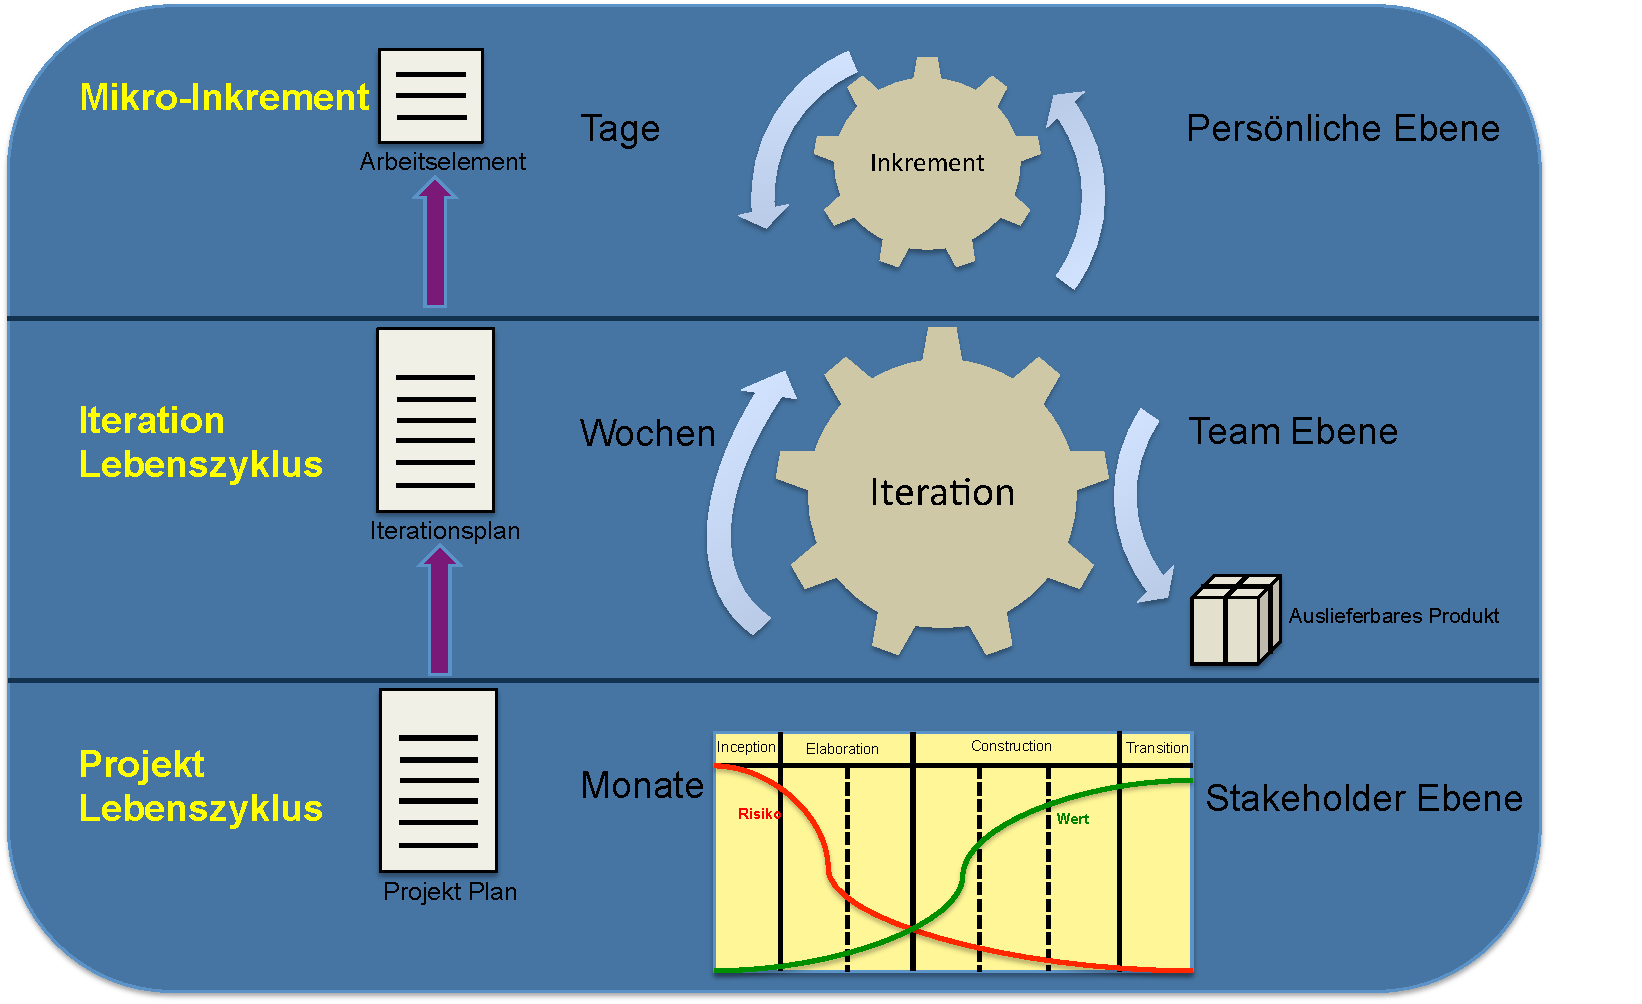
\includegraphics[width=\linewidth]{openup} %pdf, jpg, png...
  \caption{Open Up Überblick nach \cite{eclipseopenup}}
  \label{fig:openup}
\end{center}
\end{figure}

Der Open UP wird im Folgenden analysiert.

\subsection{Analyse Open UP}


Auf der persönlichen Ebene teilen sich die Teammitglieder ihre Arbeit in \textit{Mikro-Inkremente} ein. Diese stellen das Ergebnis von Stunden, bzw. wenigen Tagen Arbeit dar. Die Arbeit entwickelt sich somit ein Mikro-Inkrement weiter und der Fortschritt kann Tag für Tag nachvollzogen werden. Die Teammitglieder teilen ihre Fortschritte täglich miteinander, was die Arbeitstransparenz und das Vertrauen erhöht und die Teamarbeit fördert \cite{eclipseopenup}. \newline

Auf der Team-Ebene wird das Projekt in Iterationen unterteilt, welche einen Zeitraum von mehreren Wochen umfassen, mit dem Ziel am Ende eines Iterationszyklus ein funktionierendes Softwareinkrement zu haben. Dieses Inkrement stellt eine Version des Softwaresystems dar, welche zusätzliche oder verbesserte Funktionalitäten besitzt als die vorherige Version \cite{Basem2010}.  In jeder Iteration wird ein Iterationsplan angefertigt,  der vorgibt, was in dieser Iteration geliefert werden muss und auf welchen sich das Team verpflichten muss \cite{freudenreichevaluierung}.

Auf Stakeholder-Ebene wird diesen durch den \textit{Projektlebenszyklus} die Möglichkeit gegeben, die Projektfinanzierung, den Umfang, das Risiko und andere Aspekte des Prozesses zu kontrollieren.
Der Open UP teilt den \textit{Projektlebenszyklus} in die vier Phasen \textit{Inception}, \textit{Elaboration}, \textit{Construction} und \textit{Transition} ein, über welche Abbildung \ref{fig:Phasen} einen Überblick gibt \cite{eclipseopenup}.

\begin{figure}[htp]
\begin{center}
  \includegraphics[width=\linewidth]{Lebenszyklusopenup} %pdf, jpg, png...
  \caption{Phasen Open UP nach \cite{eclipseopenup}}
  \label{fig:Phasen}
\end{center}
\end{figure}


In jeder Phase finden eine oder mehrere Iterationen statt und werden mit einem Meilenstein abgeschlossen \cite{Basem2010}. In der Phase \textit{Inception} ist dies der Zielsetzung- Meilenstein, in der Phase \textit{Elaboration} der Architektur- Meilenstein, in der Phase \textit{Construction} der Einsatzfähigkeit- Meilenstein und in der Phase \textit{Transition} der Produkt- Release- Meilenstein.Tabelle \ref{tab:tab1} zeigt die Abläufe in den Iterationen in den einzelnen Phasen und die zugehörigen Zielstellungen.
\begin{longtable}{|p{7cm}|p{8cm}|}
\hline
Vorlagenmodell Iterationen & Zielsetzung der Phase \\
\hline
Inception Phase Iteration 
\begin {itemize}
\item Iteration starten 
 \item  Iteration planen und verwalten
 \item  Anforderungen festlegen und verfeinern 
  \end{itemize}
   &
  
  \begin {itemize}
\item Verstehen, was zu bauen ist
 \item Die wichtigsten Systemfunktionen verstehen 
\item Mindestens eine mögliche Lösung bestimmen
\item Kosten, Zeitplan und Risiken verstehen, welche mit dem Projekt verbunden sind
  \end{itemize}

 \\
\hline
 Elaboration Phase Iteration 
   \begin {itemize}
   \item Iteration planen und verwalten
   \item Anforderungen erheben und verfeinern
   \item Architektur definieren
   \item Lösung entwickeln
   \item Testlösung
   \item Laufende Aufgaben
   
  \end{itemize}

  & 
     \begin {itemize}
   \item Ein detaillierteres Verständnis der Anforderungen einholen
   \item Architektur designen, implementieren und validieren
   \item  Wesentliche Risiken mindern und genauen Zeitplan und Kostenschätzungen erstellen
    \end{itemize}
 \\
\hline
\hline
Construction Phase Iteration 
   \begin {itemize}
   \item Iteration planen und verwalten
   \item Anforderungen erheben und verfeinern
     \item Lösung entwickeln
   \item Testlösung
   \item Laufende Aufgaben

\end{itemize}

&
   \begin {itemize}
\item Komplettes Produkt iterativ entwickeln, welches am Ende bereit ist an seine Nutzer ausgeliefert zu werden
\item Entwicklungskosten minimieren und einen gewissen Grad an Parallelität erzielen 
\end{itemize}

 \\
\hline
Transition Phase Iteration 

   \begin {itemize}

 \item Iteration planen und verwalten
     \item Lösung entwickeln
   \item Testlösung
   \item Laufende Aufgaben

 \end{itemize}

 
  &
  
     \begin {itemize}
      \item Beta-Test, um zu überprüfen, dass die Erwartungen der Benutzer erfüllt sind 
     \item Zustimmung der Stakeholder einholen, dass Bereitstellung abgeschlossen ist
      \end{itemize}

\\

\hline

\caption{Iterationen und Zielstellungen der Phasen in Open UP \cite{eclipseopenup}}
\label{tab:tab1}
\end{longtable}






Abbildung \ref{fig:RollenOpenUp} gibt einen Überblick über die verschiedenen Rollen in Open UP. Die Rolle \textit{Analyst} stellt den Kunden und Endnutzer dar. Die Aufgaben des \textit{Analysten} bestehen aus dem Sammeln von Informationen von den Stakeholdern, um das Problem, welches es zu lösen gilt, zu verstehen. Weiterhin erstellt er Anforderungen und setzt Prioritäten für diese \cite{OpenUPProcess}.\newline
Der \textit{Tester} ist für sämtliche Testaktivitäten verantwortlich. Diese umfassen die Ermittlung, Festlegung, Umsetzung und Durchführung der erforderlichen Tests sowie die Protokollierung und Analyse der Ergebnisse \cite{OpenUPProcess}.
Der \textit{Entwickler} entwickelt einen Teil des Systems und muss hierbei sicherstellen, dass dieser in die Gesamtarchitektur passt. Er muss eventuell Prototypen des User-Interface anfertigen und anschließend die Komponenten implementieren, testen und integrieren \cite{OpenUPProcess}.\newline
Der \textit{Architekt} ist für die Definition der Software-Architektur verantwortlich, d.h. er trifft alle wichtigen technischen Entscheidungen, die die gesamte Entwicklung und Umsetzung des Systems betreffen \cite{OpenUPProcess}.\newline
Der \textit{Projekt Manager} führt die Planung des Projektes durch, koordiniert die Zusammenarbeit zwischen allen Beteiligten und achtet darauf, dass das Projektteam die Erfüllung der Projektziele stets im Auge behält \cite{OpenUPProcess}.\newline
Die Rolle des \textit{Stakeholders} schließt alle Interessengruppen ein, deren Ansprüche durch das Projekt erfüllt werden müssen. \newline

\begin{figure}[htp]
\begin{center}
  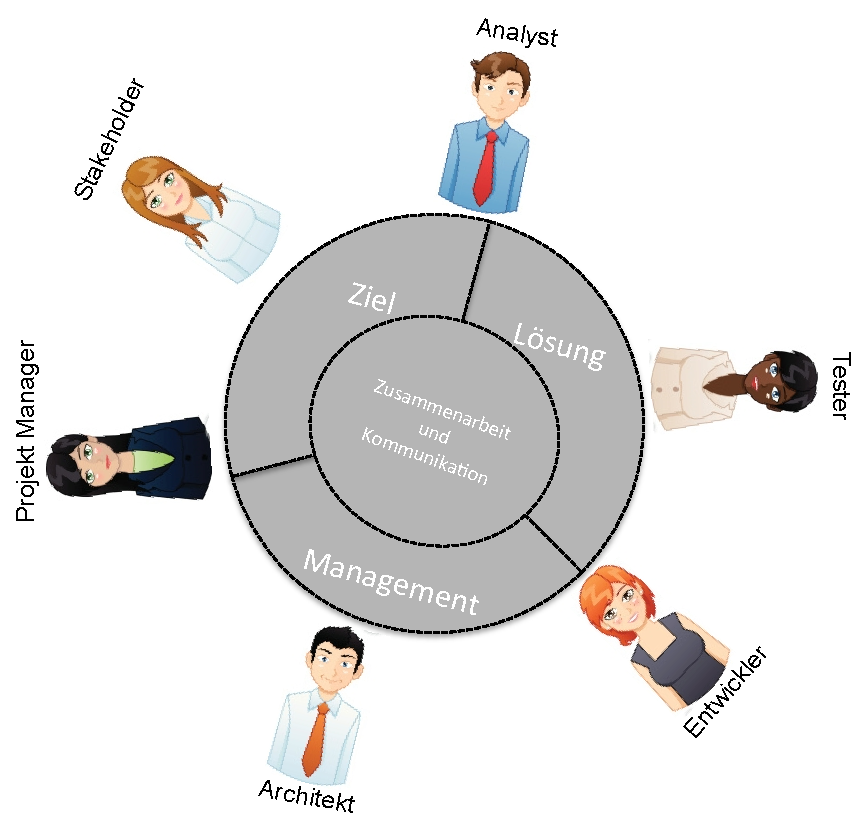
\includegraphics[scale=0.6]{RollenOpenUp} %pdf, jpg, png...
  \caption{Rollen in Open UP nach \cite{openup}}
  \label{fig:RollenOpenUp}
\end{center}
\end{figure}

Eine Task bezeichnet in Open UP die Arbeitseinheit einer Rolle, welche von dieser durchgeführt werden soll. Insgesamt gibt es 18 Tasks, welche von den verschiedenen Rollen entweder als Primär-Darsteller (der Verantwortliche für die Durchführung der Aufgabe) oder als zusätzlicher Darsteller (Unterstützung und Bereitstellung von Informationen, die in der Task- Ausführung verwendet werden), durchgeführt werden. Hierdurch wird der kollaborative Charakter von Open UP gefestigt \cite{eclipseopenup}.

Ein Artefakt ist etwas, das hergestellt, modifiziert oder durch eine Task verwendet wird. Rollen sind 
für die Erstellung und Aktualisierung von Artefakten verantwortlich. Artefakte stellen eine Versionskontrolle während des gesamten Projektlebenszyklus dar. Die 17 Artefakte in OpenUP gelten als die wesentlichen Artefakte, welche ein Projekt verwenden sollte, um produkt- und projektbezogene Informationen zu erfassen. Die Informationen müssen hierbei nicht mit formalen Artefakten festgehalten werden. Dies kann auch informell, z.B durch White-Boards oder Meeting-Notizen geschehen. Es können die Open UP Artefakte oder eigene Artefakte verwendet werden \cite{eclipseopenup}.

\subsection{Imperative Modellierung Open UP}

 \subsubsection{Phasen Open UP}

In Abbildung \ref{fig:OpenUpPhasen} sind die vier Phasen des Open UP modelliert. Da jede Phase in Iterationen mehrmals durchlaufen werden kann, gibt es nach jeder Phase ein XOR-Gateway, welches im Falle einer weiteren notwendigen Iteartion zum Anfang der Phase zurück führt. Diese kann sodann erneut durchlaufen werden.

\begin{figure}[htp]
\begin{center}
  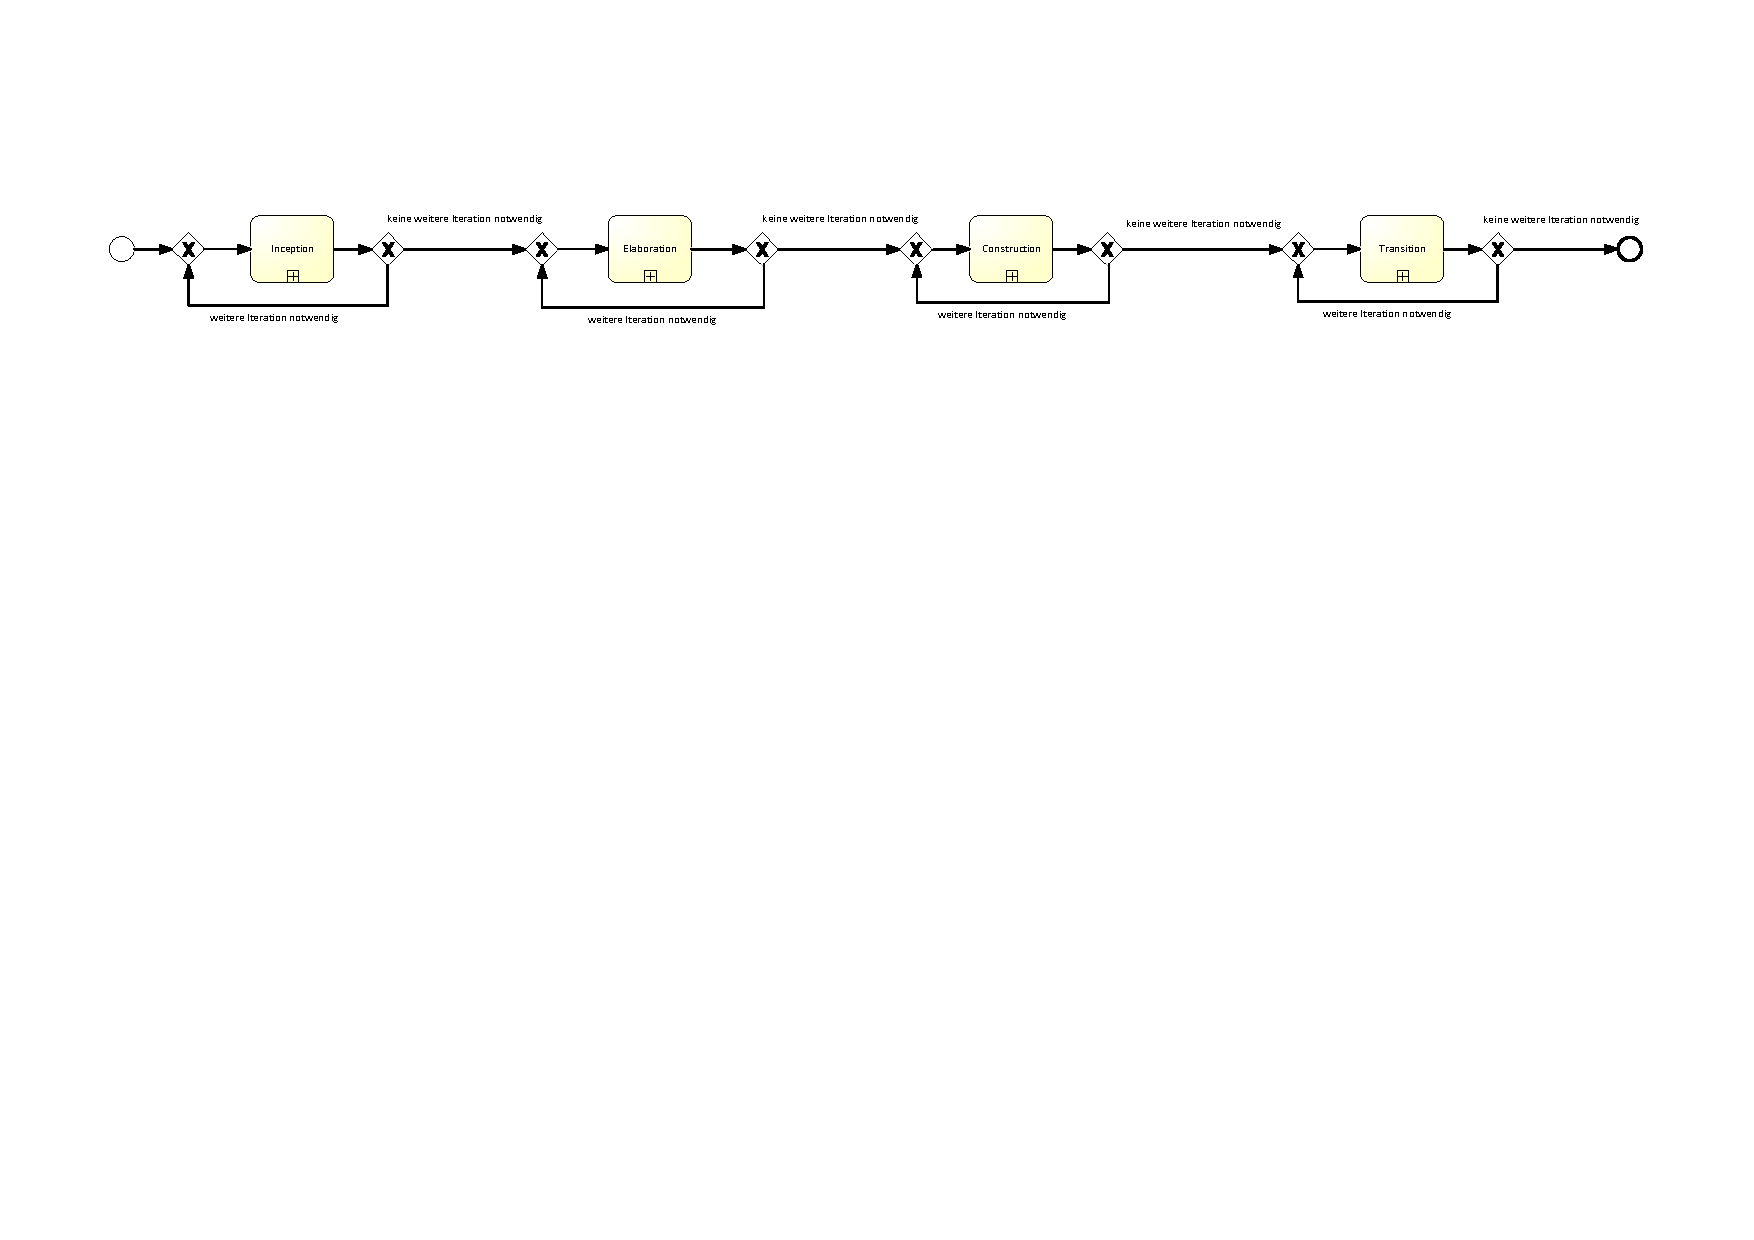
\includegraphics[width=\linewidth]{OpenUpPhasen} %pdf, jpg, png...
  \caption{Phasen Open UP- imperativ}
  \label{fig:OpenUpPhasen}
\end{center}
\end{figure}

Abbildung \ref{fig:OpenUpInception} zeigt die imperative Modellierung der Phase Inception. Die Aktivität \textit{Projekt planen und managen} kann parallel zu allen anderen Aktivitäten des Modells ausgeführt werden.\newline
Nach Ausführung der Aktivität \textit{Iteration planen} werden die Aktvitäten \textit{Anforderungen identifizieren und aufbereiten} und \textit{auf technisches Vorgehen einigen} parallel zueinander ausgeführt.

\begin{figure}[htp]
\begin{center}
  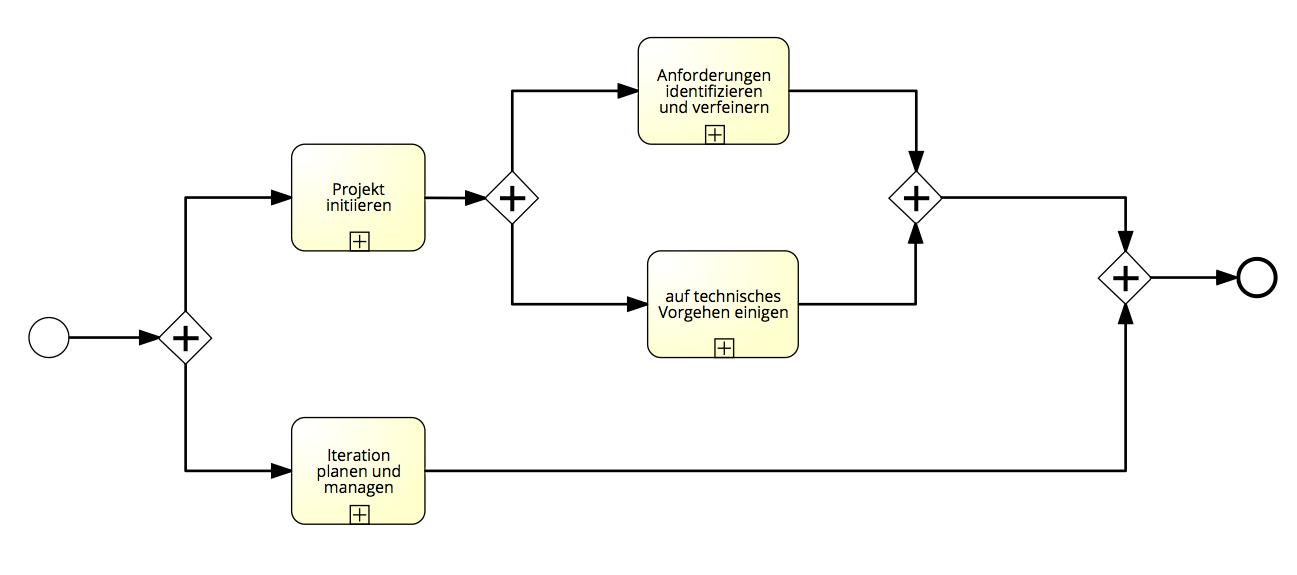
\includegraphics[scale=0.8]{OpenUpInception} %pdf, jpg, png...
  \caption{Phasen Open UP Unterprozess Inception- imperativ}
  \label{fig:OpenUpInception}
\end{center}
\end{figure}

In Abbildung \ref{fig:OpenUpElaboration} ist die imperative Modellierung der Phase Elaboration abgebildet. Die sechs Aktivtäten \textit{Anforderungen identifizieren und verfeinern, Architektur entwickeln, Lösungsinkrement entwickeln, Lösung testen, Iteration planen und managen} sowie \textit{weitere Aufgaben erledigen} werden parallel zueinander ausgeführt.

\begin{figure}[htp]
\begin{center}
  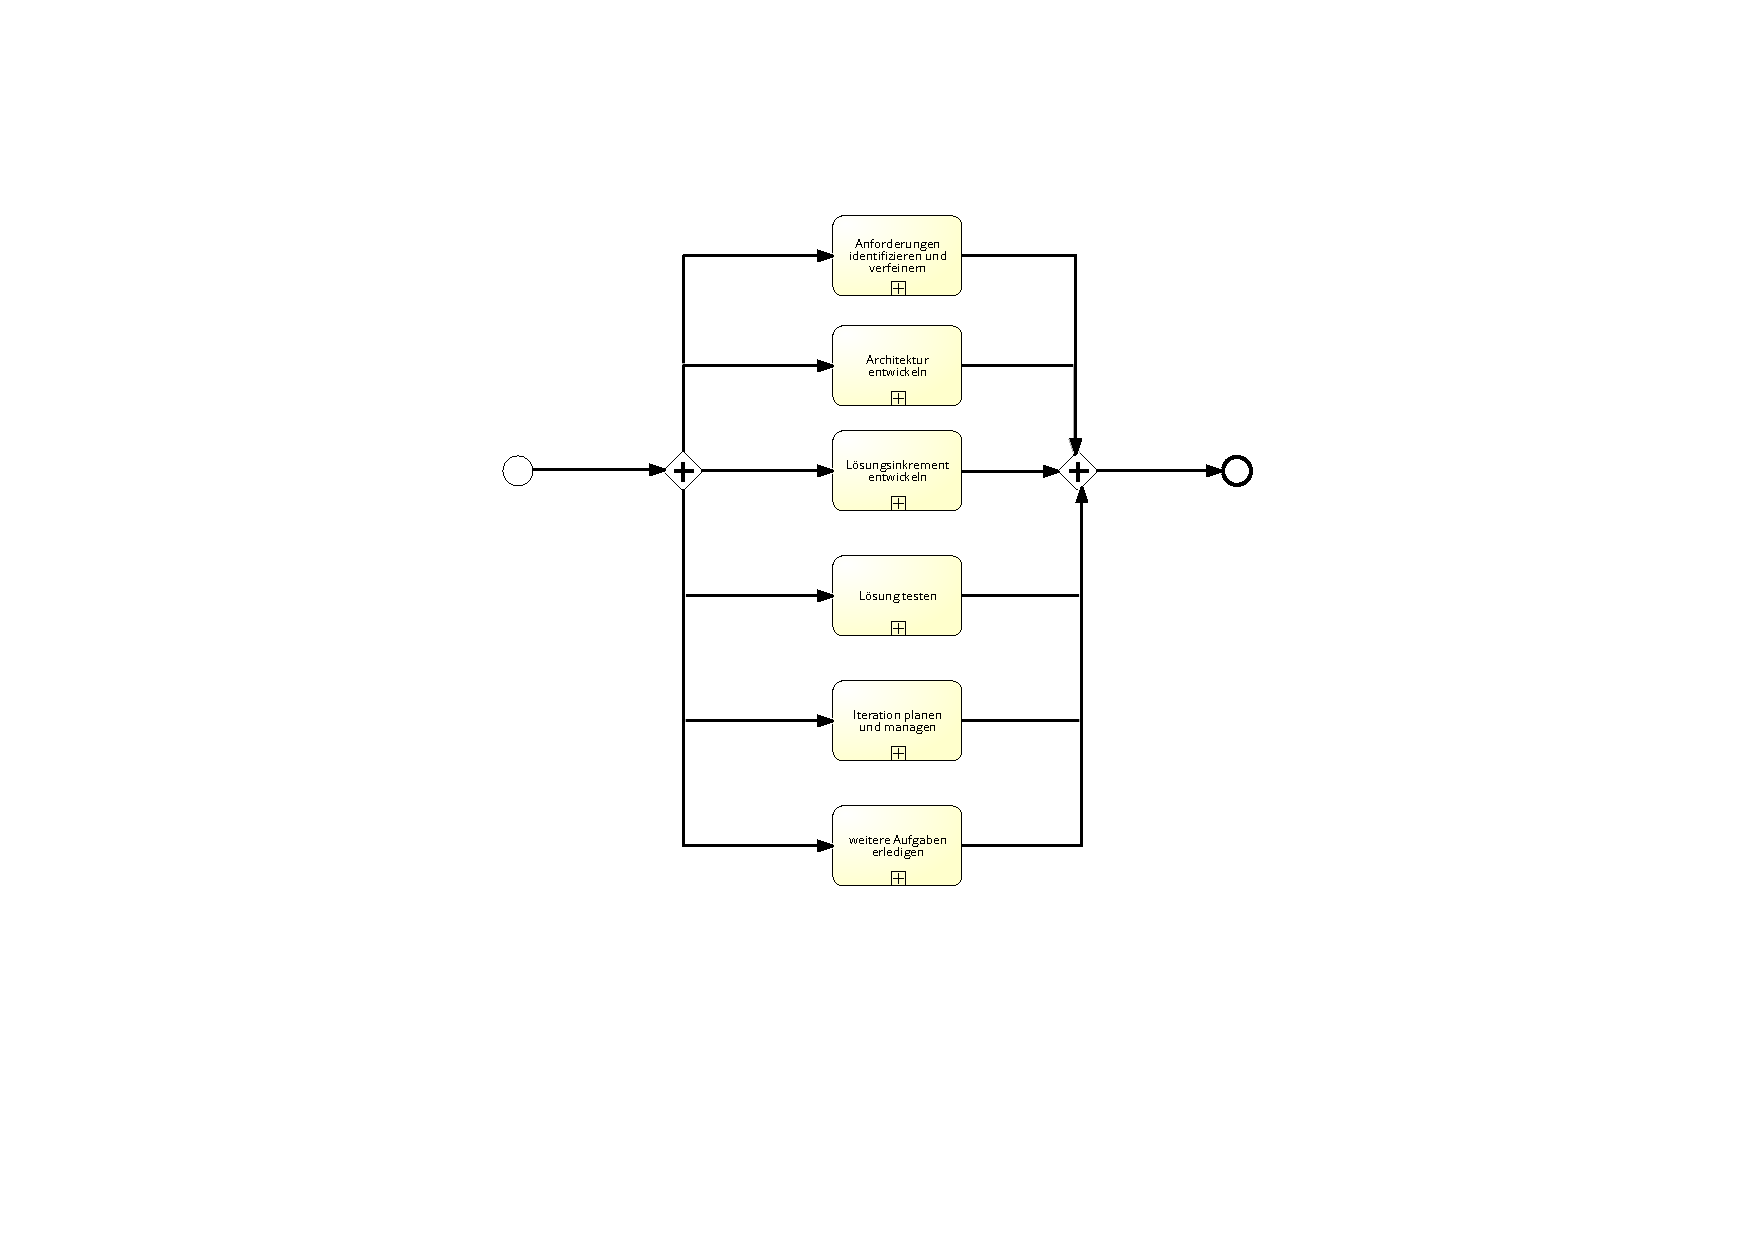
\includegraphics[scale=0.8]{OpenUpElaboration} %pdf, jpg, png...
  \caption{Phasen Open UP Unterprozess Elaboration- imperativ}
  \label{fig:OpenUpElaboration}
\end{center}
\end{figure}

Die imperative Modellierung der Phase Construction kann Abbildung \ref{fig:OpenUpConstruction} entnommen werden. Hier werden die sechs Aktivitäten \textit{Anforderungen identifizieren und verfeinern, Lösungsinkrement entwickeln, Lösung testen, Iteration planen und managen, weitere Aufgaben erledigen} und \textit{Produktdokumentation und Training erstellen} nebeneinander parallel ausgeführt.
\begin{figure}[htp]
\begin{center}
  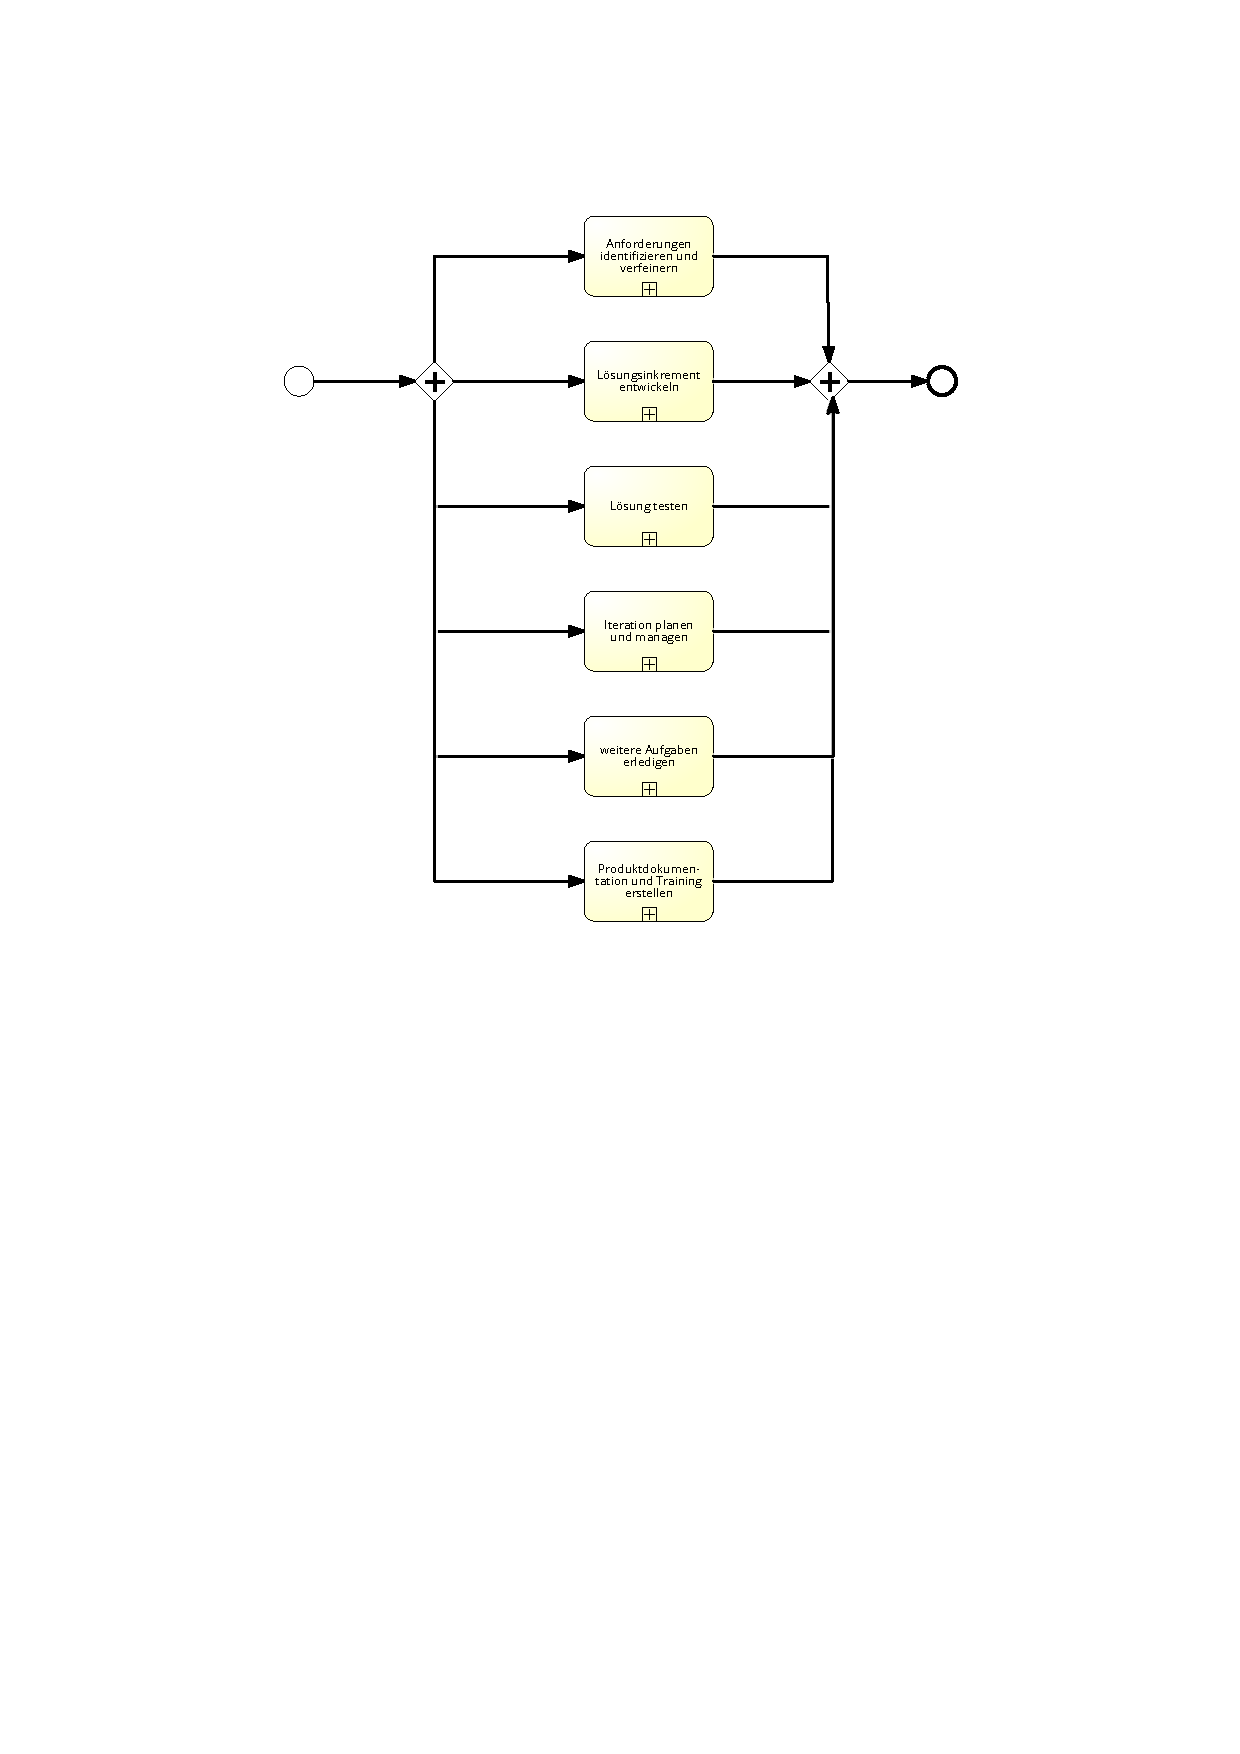
\includegraphics[scale=0.8]{OpenUpConstruction} %pdf, jpg, png...
  \caption{Phasen Open UP Unterprozess Construction- imperativ}
  \label{fig:OpenUpConstruction}
\end{center}
\end{figure}

Abbildung \ref{fig:OpenUpTransition} kann die imperative Modellierung der Phase Transition entnommen werden.\newline
Die Phasen \textit{Anforderungen identifizieren und verfeinern, Produkt Training durchführen, Lösungsinkrement entwickeln, Lösung testen, Iteration planen und managen, weitere Aufgaben erledigen, Produktdokumentation und Training abschließen} sowie \textit{Release für die Produktion freigeben} werden parallel zueinander ausgeführt.

\begin{figure}[htp]
\begin{center}
  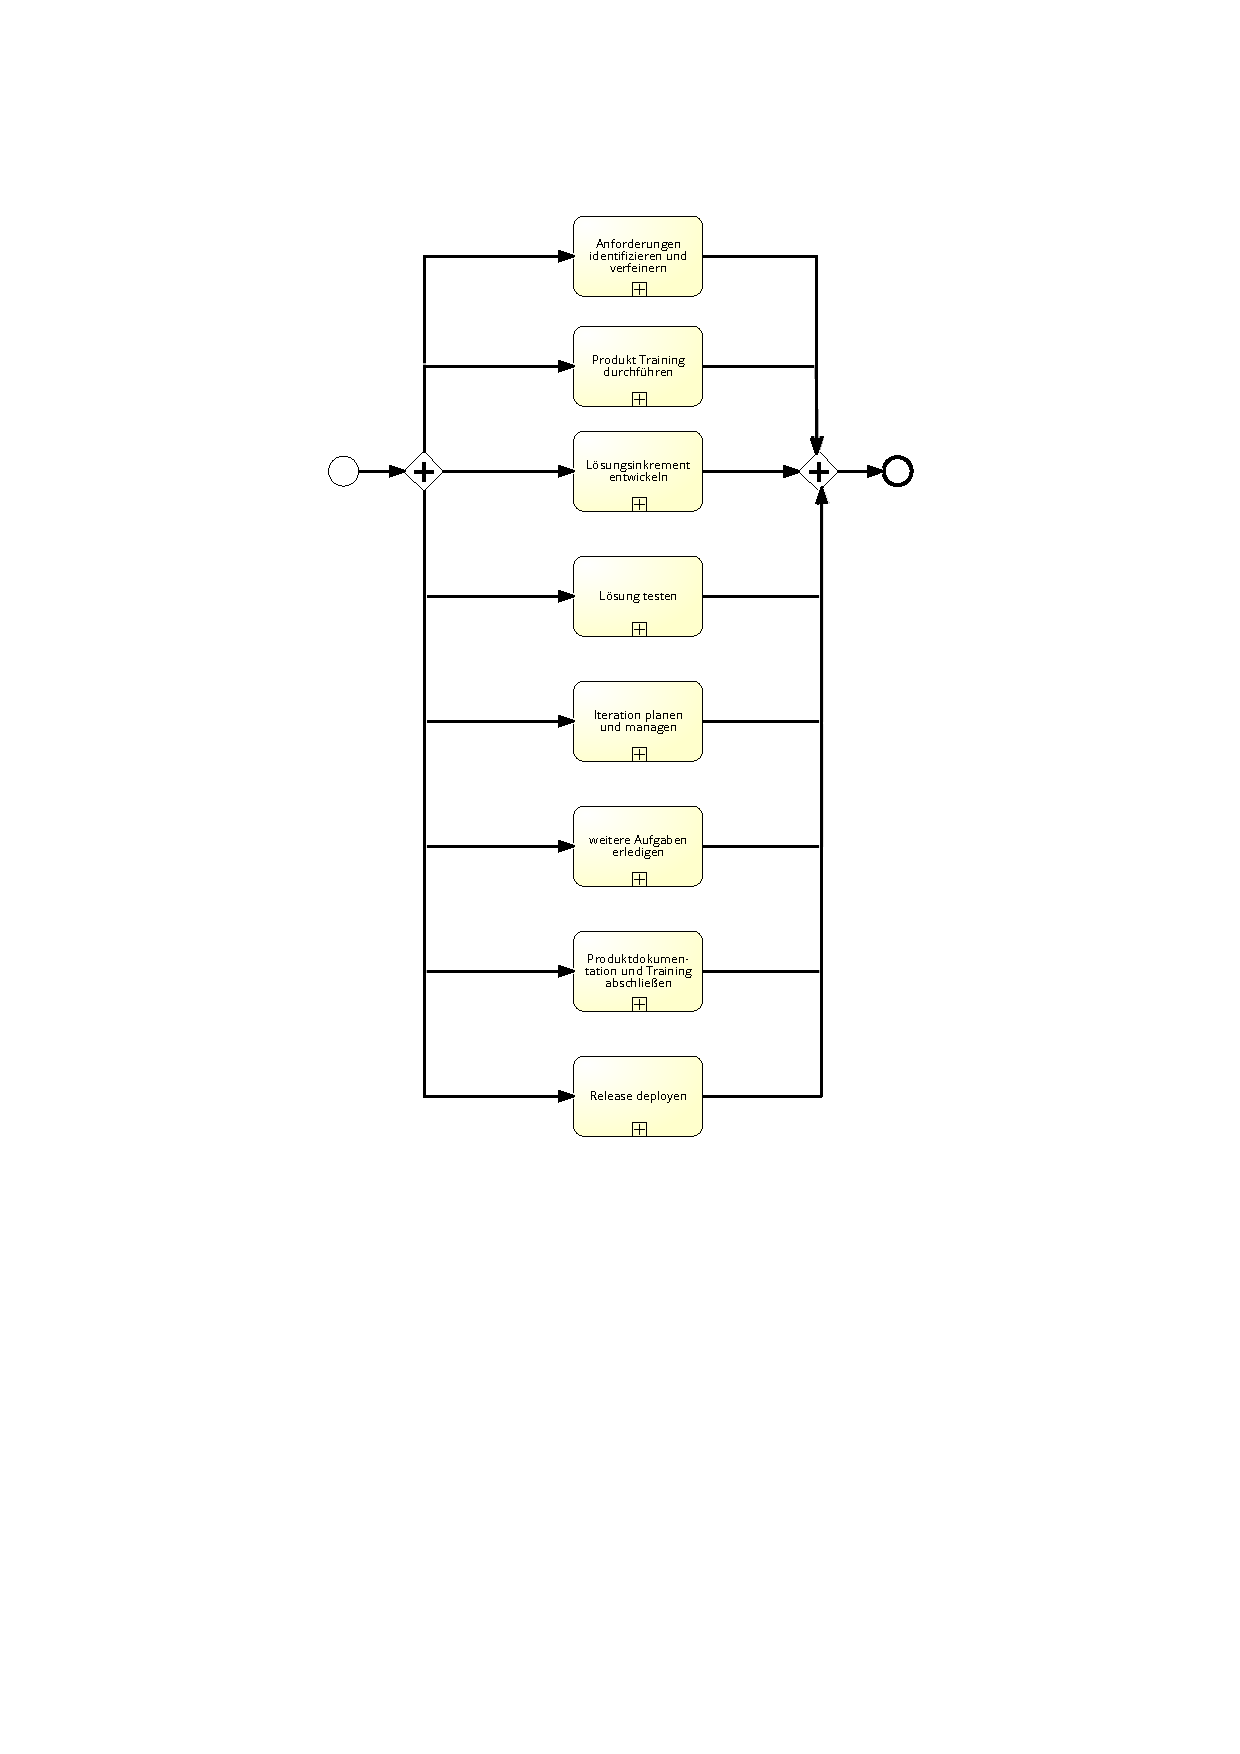
\includegraphics[scale=0.8]{OpenUpTransition} %pdf, jpg, png...
  \caption{Phasen Open UP Unterprozess Transition- imperativ}
  \label{fig:OpenUpTransition}
\end{center}
\end{figure}



Im weiteren Verlauf wird aus jeder der vier Phasen Inception, Elaboration, Construction und Transition des Open UP jeweils ein Unterprozess modelliert, da die Abbildung aller Unterprozesse aus jeder Phase den Rahmen der Arbeit sprengen würde. \newline
Somit wird für die Phase Inception der Unterprozess \textit{Iteration planen und managen}, für die Phase Elaboration der Unterprozess \textit{Anforderungen identifizieren und verfeinern}, für die Phase Construction der Unterprozess \textit{Release deployen} und für die Phase Transition der Unterprozess \textit{Produktdokumentation und Training erstellen} modelliert. Außerdem wird der in den drei Phasen Elaboration, Construction und Transition wiederkehrende Unterprozess \textit{Lösungsinkrement entwickeln} modelliert.

\subsubsection{Lösungsinkrement entwickeln}

Im Unterprozess \textit{Lösungsinkrement entwickeln} geht es um das Design, die Implementierung, das Testen und die Integration der Lösung für eine Anforderung in einem bestimmten Kontext. Sie tritt genauso viele Male auf, wie es Arbeitsaufgaben gibt, die in einer Iteration entwickelt werden müssen.
 Handelt es sich um eine typische Veränderung wird zunächst eine Lösung designt und anschließend ein Entwickeltest implementiert. Bei einer trivialen Änderung an der bestehenden Implementierung kann diese auch direkt in der bestehenden Architektur vorgenommen werden. \newline
 Sobald die Fragen der technischen Umsetzung geklärt sind, werden Entwicklertests implementiert, um die Implementierung zu verifizieren. Anschließend werden diese Entwicklertests ausgeführt.\newline
 Falls bei der Ausführung der Tests Fehler ersichtlich werden, muss eine Lösung für diesen Fehler implementiert werden und die Entwicklertests müssen erneut ausgeführt werden. Dies wird solange wiederholt, bis alle Tests bestanden sind.\newline
 Auch wenn alle Tests bestanden werden, sollte der Entwurf an dieser Stelle nochmals überdacht werden. Falls hier beschlossen wird, dass der Code überarbeitet werden muss, muss im Prozess zurückgegangen werden und erneut eine Lösung designt werden, da eine Änderung des Codes die Implementation und die Entwicklertests beeinflussen könnte.\newline
 Da es am Besten ist die Implementierungsteile so klein wie möglich zu halten, sollte zunächst eine kleine Design-Lösung für einen Teil der Arbeitsaufgabe entwickelt werden. Anschließend sollte dies für weitere kleine Teile solange wiederholt werden, bis die gesamte Arbeitsaufgabe implementiert ist. \newline
 In Abbildung \ref{fig:Develop} ist die imperative Modellierung von \textit{Lösungsinkrement entwickeln} abgebildet.\newline
 Die XOR-Verknüpfung am Anfang führt im Falle einer trivialen Änderung zur sofortigen Ausführung der Aktivität \textit{Entwicklertest implementieren}. Falls es sich jedoch um eine typische Änderung handelt, muss zuvor die Aktivität \textit{Lösung designen} ausgeführt werden. Im Anschluß an \textit{Entwicklertest implementieren} muss die Aktivität \textit{Entwicklertest ausführen} durchgeführt werden.\newline
 Hiernach wird im Falle eines fehlgeschlagenen Tests zunächst eine \textit{Lösung implementiert} und anschließend erneut der \textit{Entwicklertest ausgeführt}. \newline
 Wenn der Test bestanden ist muss am XOR-Gateway entschieden werden, ob der Code gut designt ist. Falls nein, muss erneut eine Lösung designt werden. Falls doch, kann der Code integriert werden. Ist die Arbeit vollständig erledigt, so ist der Prozess beendet. Wenn jedoch noch weitere Arbeit vorhanden ist, beginnt er von vorne.
 
 
\begin{figure}[htp]
\begin{center}
  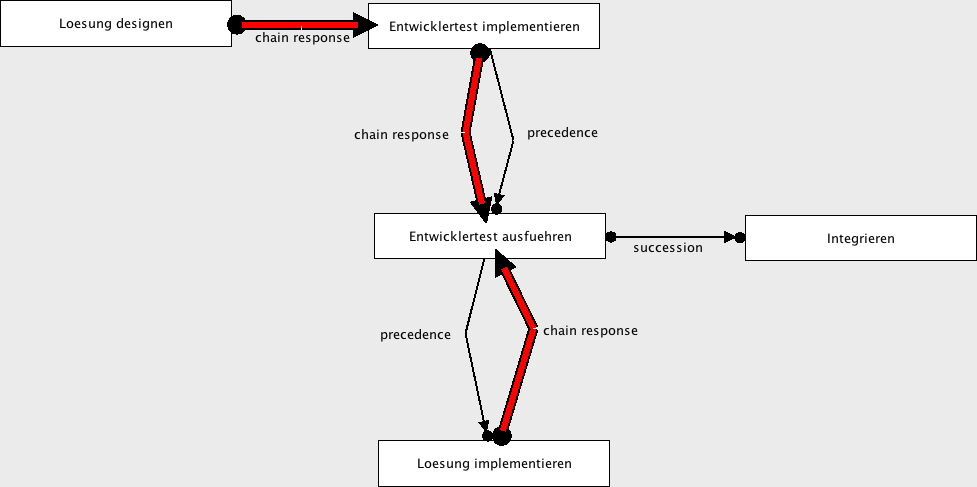
\includegraphics[width=\linewidth]{DevelopSolution} %pdf, jpg, png...
  \caption{Lösungsinkrement entwickeln imperativ}
  \label{fig:Develop}
\end{center}
\end{figure}

\subsubsection{Iteration planen und managen- Inception}

Die Aktivität \textit{Iteration planen und managen} wird während des gesamten Projektlebenszyklus ausgeführt. Ihr Ziel ist es, Risiken und Probleme früh genug zu identifizieren, damit diese entschärft werden können, um die Ziele für die Iteration festzulegen und das Team dabei zu unterstützen, diese zu erreichen.\newline
Die Iteration wird durch den Projektmanager und das Team gestartet. Hier findet die Priorisierung der Arbeit für eine gegebene Iteration statt. Der Projektmanager, die Stakeholder und die Teammitglieder einigen sich darauf, was während der Iteration zu entwickeln ist.\newline
Die Teammitglieder melden sich für die Arbeitsaufgaben, die während der Iteration entwickelt werden müssen. Anschließend teilt sich jedes Teammitglied seine Arbeitsaufgaben selbstständig in Arbeitseinheiten ein und schätzt den Aufwand hierfür ab.\newline
Während der Iteration trifft sich das Team regelmäßig, um den aktuellen Stand der Arbeit und eventuelle Probleme zu besprechen. \newline
Abbildung \ref{fig:PlanAndManageIterationInception-2} zeigt die imperative Modellierug von \textit{Iteration planen und managen}. \newline
Vom Projektmanager sind hierbei nacheinander die Aktivitäten \textit{Iteration planen, Umgebung vorbereiten, Iteration managen} und \textit{Ergebnsse festlegen} durchzuführen und das Team muss nacheinander die Aktivitäten \textit{Arbeitsaufgaben aussuchen, Arbeitsaufgaben in Entwicklungsaufgaben einteilen} sowie \textit{Aufwand abschätzen} ausführen. Hierbei gehen jeweils die Artefakte \textit{Arbeitseinheiten-Liste, Iterationsplan} und \textit{Risiko-Liste} in verschieden Aktivitäten als Input ein und kommen eventuel verändert als Output wieder heraus. \newline
Die Aktivität \textit{Umgebung vorbereiten} ist als Unterprozess in Abbildung \ref{fig:Umgebungvorbereiten} dargestellt. Hier müssen vom Projektmanager die Aktivitäten \textit{Prozess Maßschneidern} und \textit{Prozess deployen} sequentiell erledigt werden, während der Tool Spezialist die Aufgaben \textit{Tools aufsetzen} und \textit{Tool-Konfiguration und Implementation verifizieren} zu erledigen hat.


\begin{figure}[!htbp]
\begin{center}
  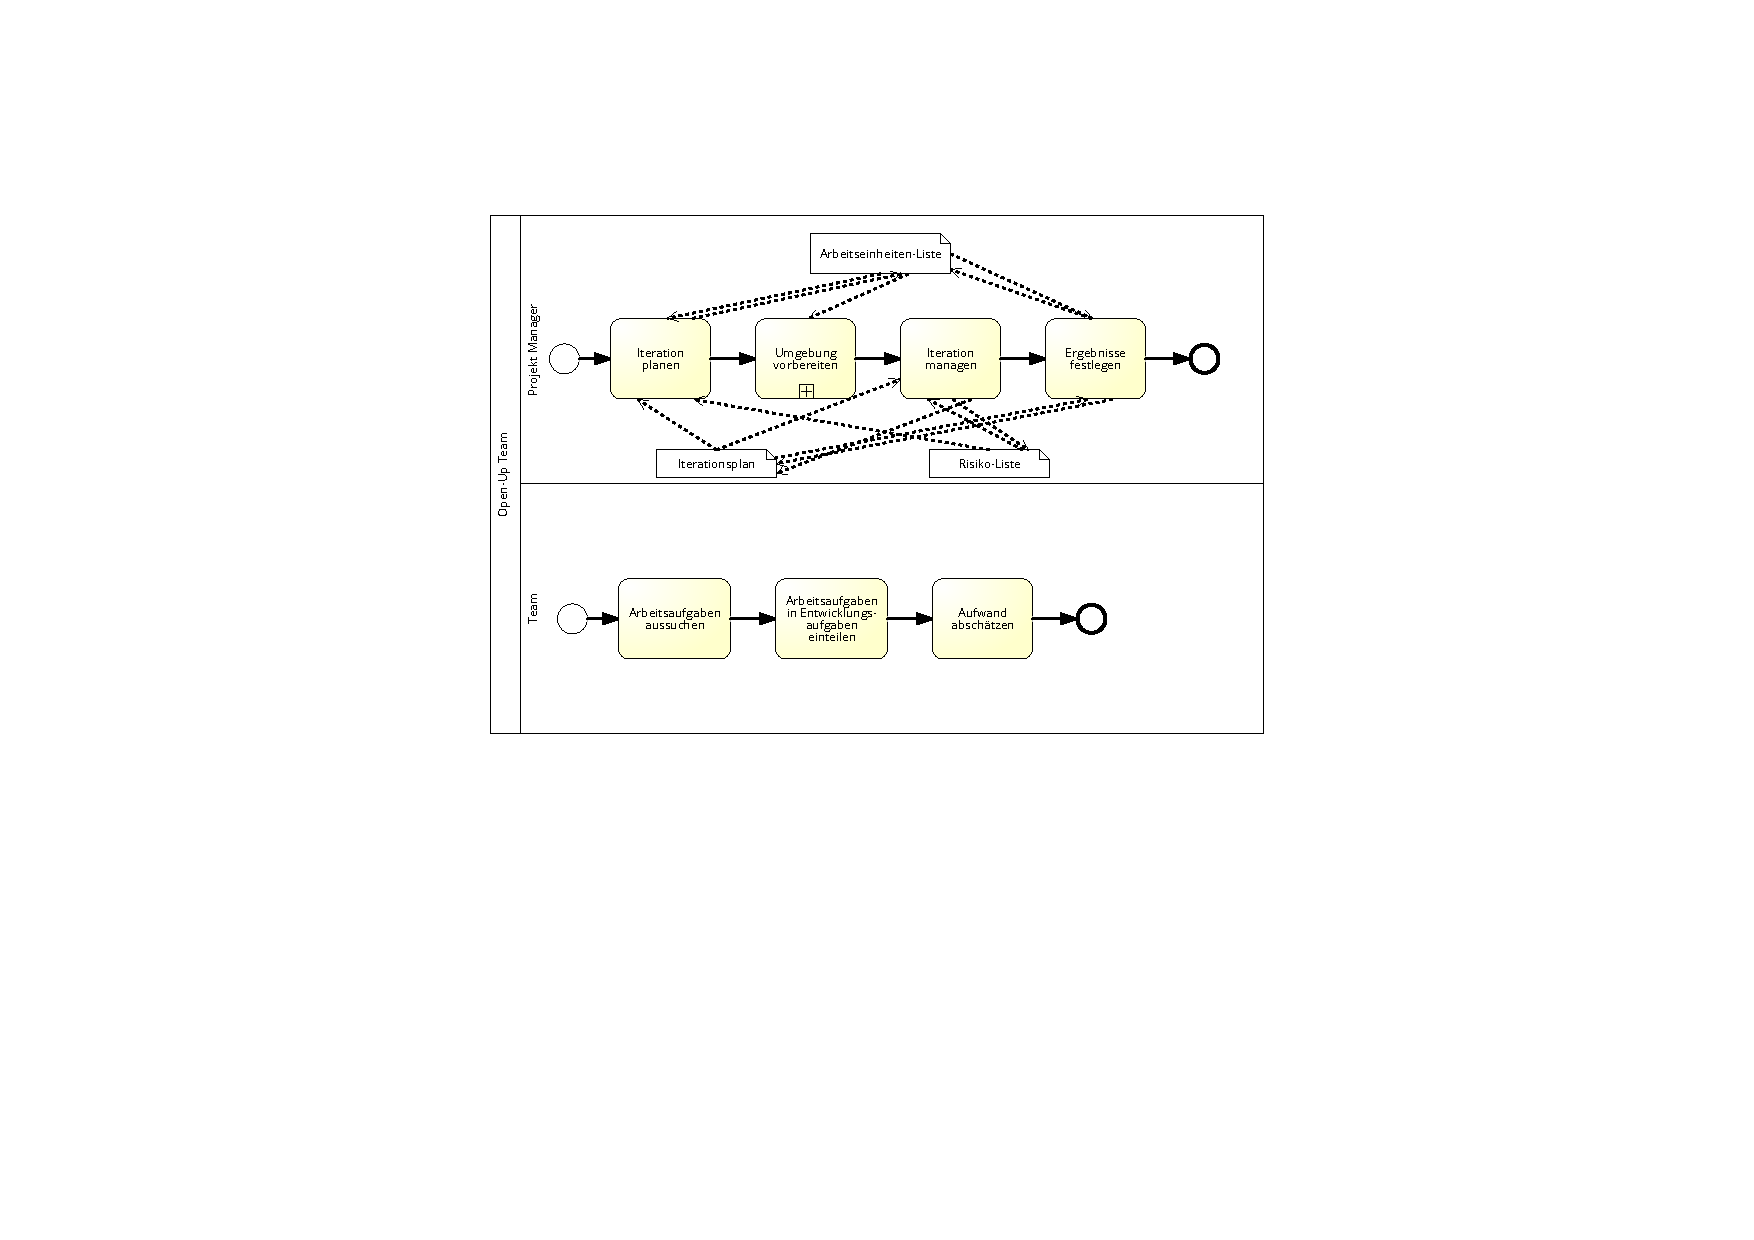
\includegraphics[scale=0.7]{PlanAndManageIterationInception-2} %pdf, jpg, png...
  \caption{Iteration planen und managen imperativ -Inception}
  \label{fig:PlanAndManageIterationInception-2}
\end{center}
\end{figure}

\begin{figure}[!htbp]
\begin{center}
  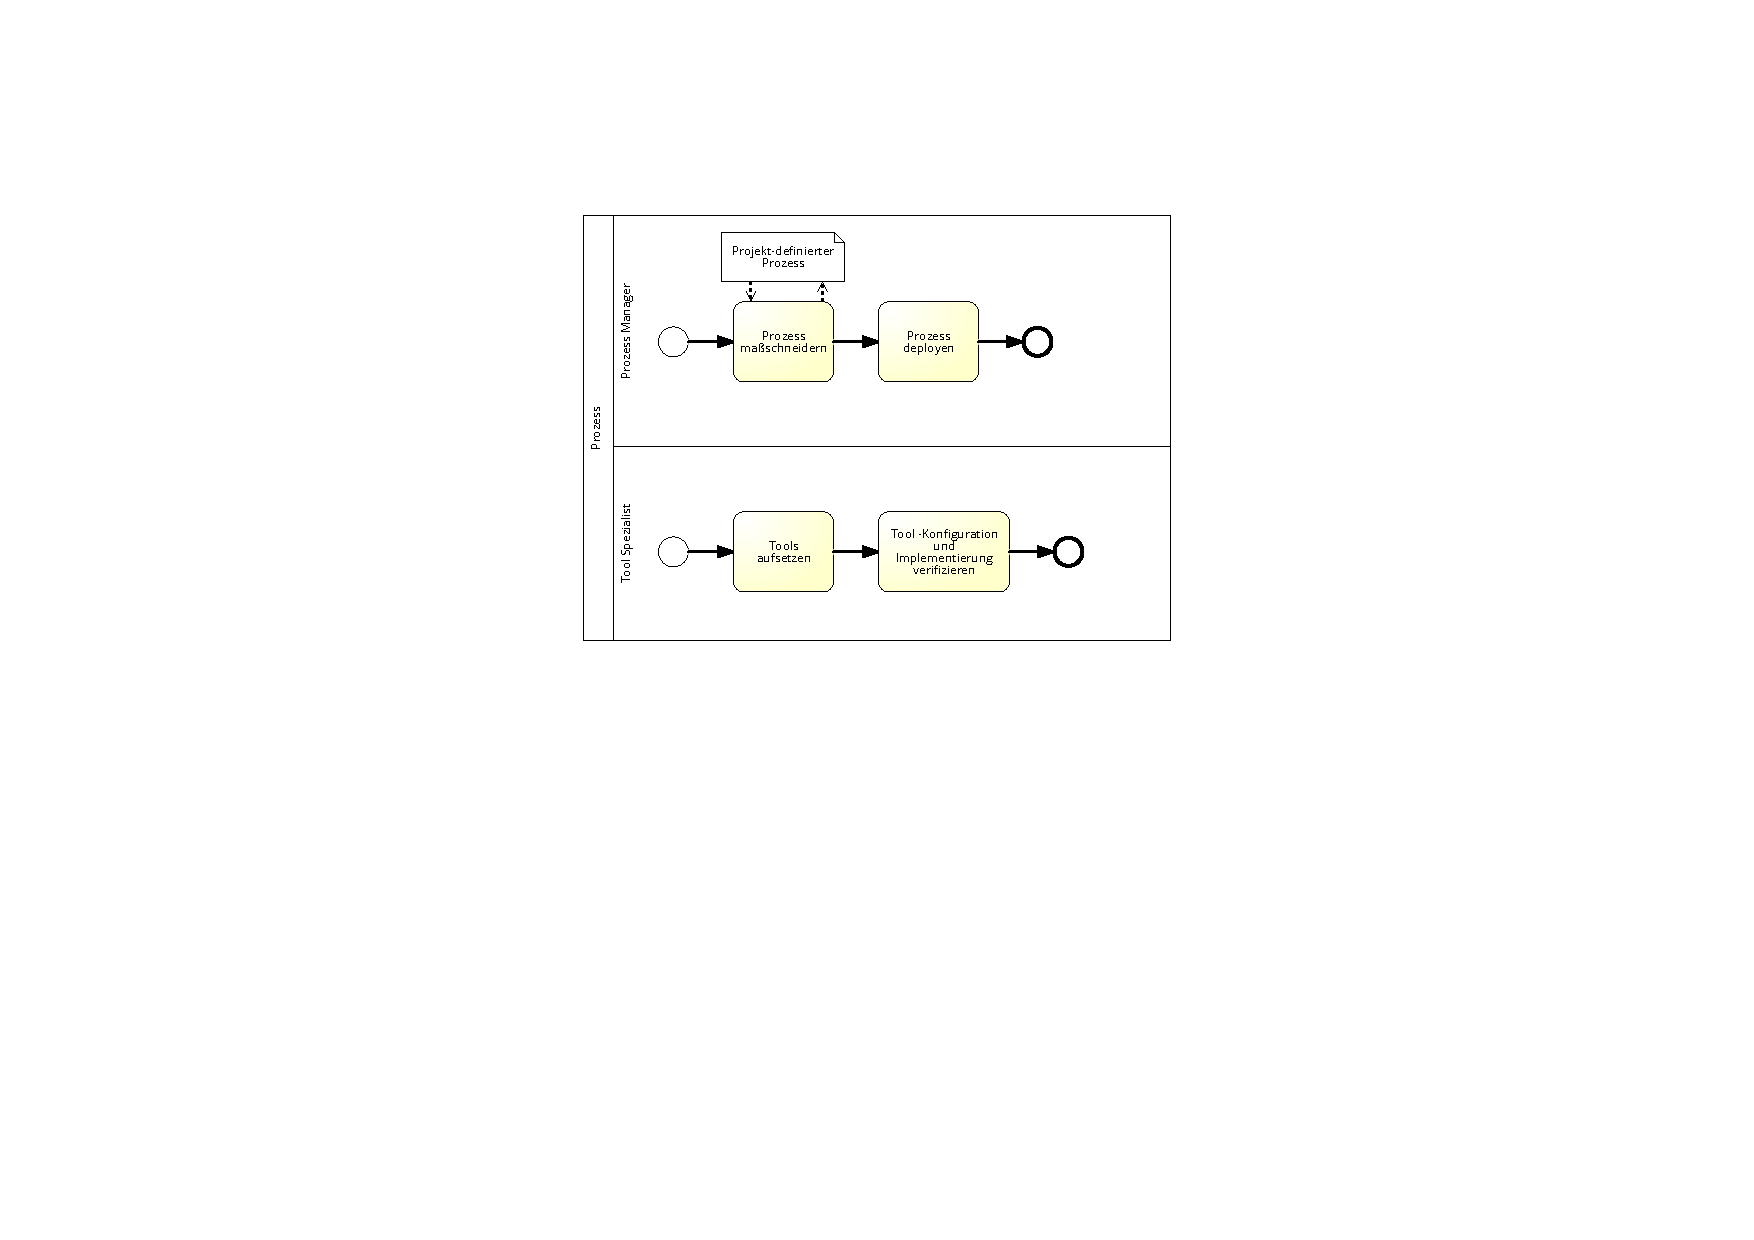
\includegraphics[scale=0.7]{Umgebungvorbereiten} %pdf, jpg, png...
  \caption{Iteration planen und managen imperativ -Inception Unterprozess Umgebung vorbereiten} 
  \label{fig:Umgebungvorbereiten}
\end{center}
\end{figure}

\clearpage


\subsubsection{Anforderungen identifizieren und verfeinern}
 Der Unterprozess \textit{Anforderungen identifizieren und verfeinern} beschreibt die Aufgaben, welche durchzuführen sind, um die Anforderungen eines Systems zu sammeln, zu analysieren und zu validieren bevor die Implemementierung und die Validierung stattfinden. Sie wird in Zusammenarbeit mit Stakeholdern und dem gesamten Entwicklungsteam ausgeführt, um sicher zu gehen, dass klare, konsistente, korrekte und nachprüfbare Anforderungen vorhanden sind.\newline
 In der Phase Elaboration liegt der Fokus hierbei auf der Definition der Lösung. Hierfür müssen diejenigen Anforderungen gefunden werden, welche für die Stakeholder am wichtigsten sind, die besonders herausfordernd oder sogar riskant sind oder eine große Bedeutung für die Architektur haben.\newline
 Dafür ist es notwendig, zunächst die funktionalen und nicht-funktionalen Anforderungen an das System zu erheben. Genau diese Anforderungen stellen dann die Basis für die Kommunikation und die Übereinstimmung zwischen den Stakeholdern und dem Entwicklungsteam dar, in Bezug auf was das System können muss, um die Wünsche der Stakeholder zu erfüllen.\newline
 Weiterhin müssen die Use-Case-Szenarien und die systemweiten Anforderungen ausführlich genug beschrieben werden, um sicher zu gehen, dass die Anforderungen richtig verstanden wurden und dass diese mit den Erwartungen der Stakeholder übereinstimmen.\newline
 Zudem müssen Testfälle und Testdaten für die Anforderungen entwickelt werden, um ein gemeinsames Verständnis für die spezifischen Bedingungen, die die Lösung erfüllen muss, zu erreichen.
 In Abbildung \ref{fig:IdentifyAndOutlineKlein} ist die imperative Modellierung von \textit{Anforderungen identifizieren und verfeinern} abgebildet. \newline
 Zunächst muss der Analyst die \textit{Anforderungen identifizieren und abgrenzen}, bevor er anschließend die \textit{Use-Case-Szenarien detaillieren} kann. Daraufhin muss er die \textit{Systemweiten Anforderungen detaillieren}, damit der Tester anschließend die \textit{Testfälle erstellen} kann.\newline
 Hier gehen bei den verschiedenen Aktivitäten die Artefakte \textit{Arbeitseinheitenliste}, \textit{Use Case}, \textit{Glossar}, \textit{Systemweite Anforderungen}, \textit{Use case Modell}, \textit{Technische Spezifikation} und \textit{Testfall} als Input hinein, bzw. als Output heraus.
 
\begin{figure}[[!htbp]
\begin{center}
  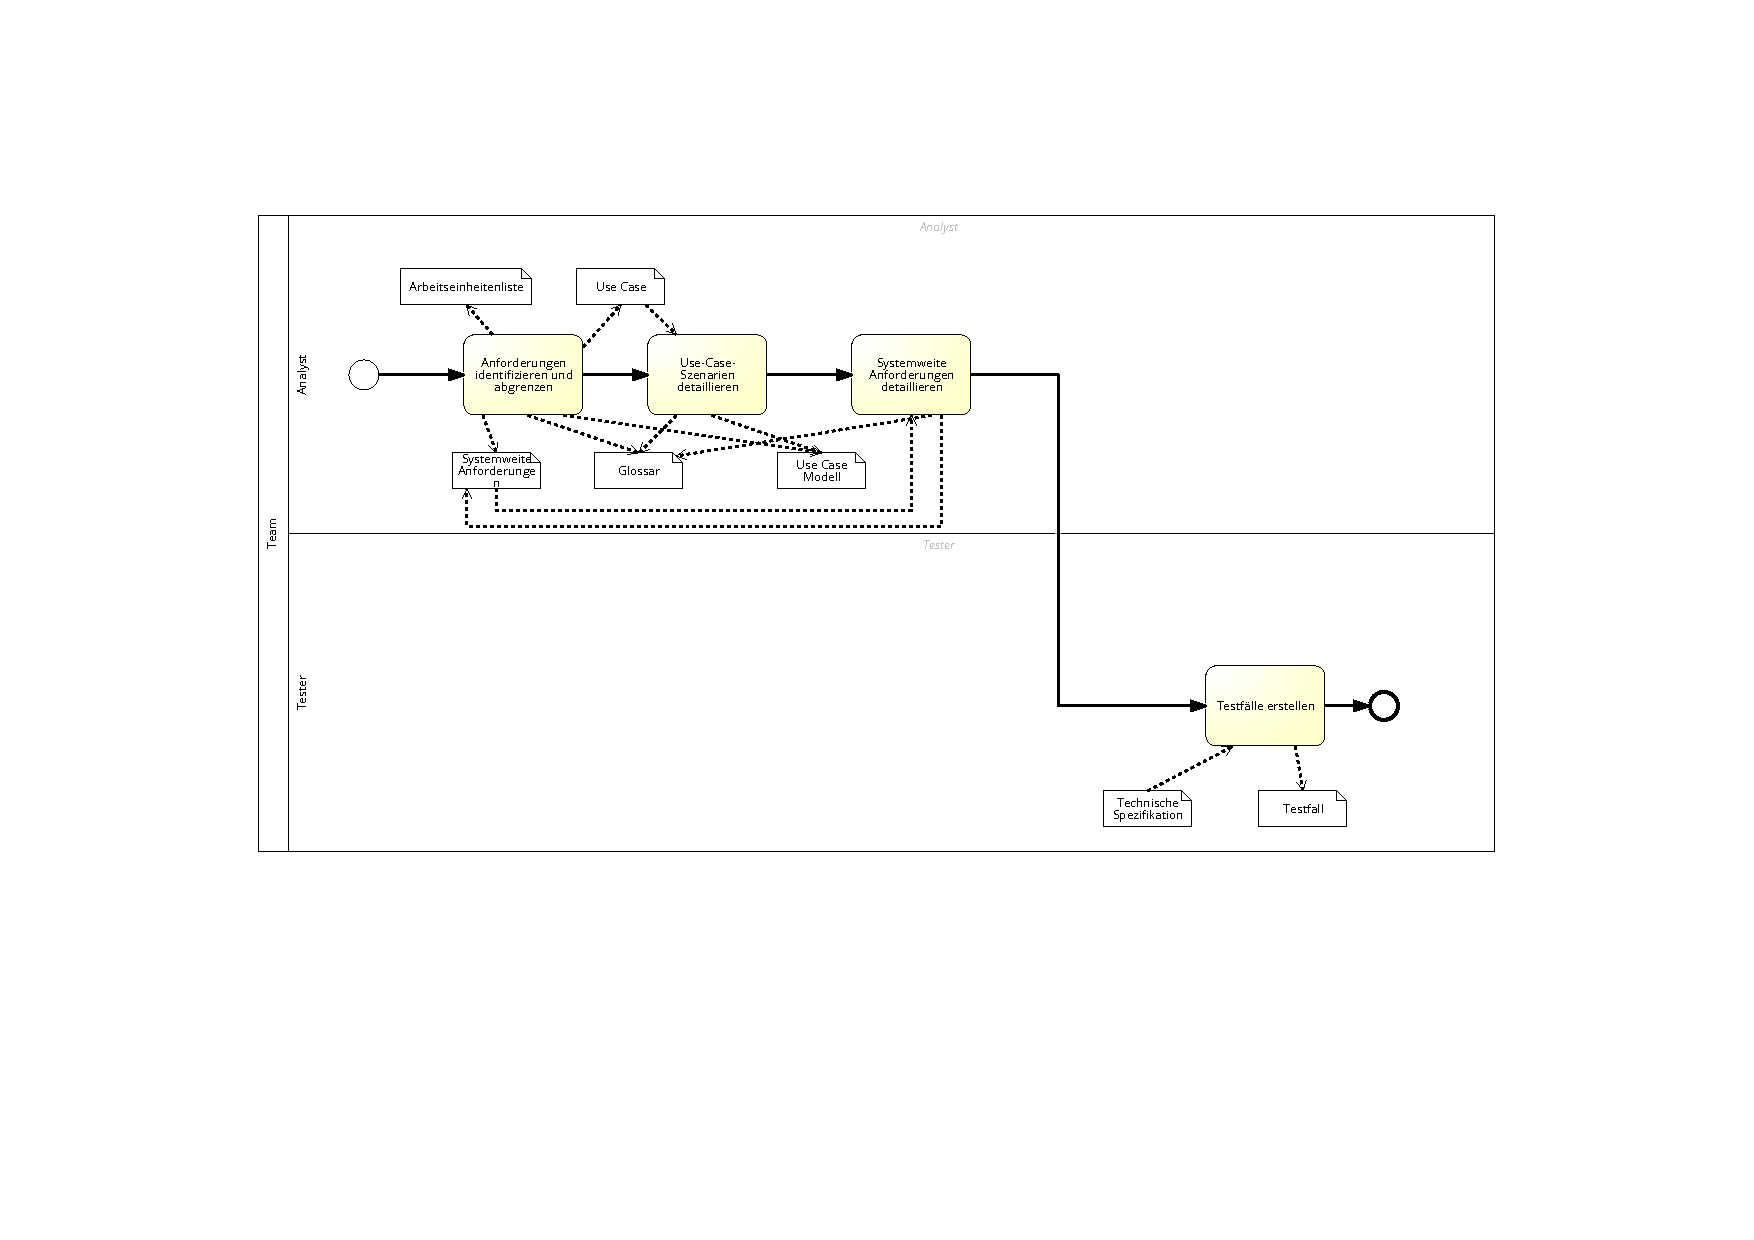
\includegraphics[width=\linewidth]{IdentifyAndOutlineKlein} %pdf, jpg, png...
  \caption{Anforderungen identifizieren und verfeinern-Elaboration}
  \label{fig:IdentifyAndOutlineKlein}
\end{center}
\end{figure}


\subsubsection{Produktdokumentation und Training erstellen-Construction}
 Das Ziel des Unterprozesses \textit{Produktdokumentation und Training erstellen} ist es, die Produktdokumentation und Trainingsmaterial vorzubereiten. Da die Produktdokumentation oftmals erst nach Abschluss der Entwicklungstätigkeiten erstellt wird, muss sichergestellt werden, dass die Funktionen die während einer Release entwickelt werden klar dokumentiert werden, solange die Funktionalität noch frisch in den Köpfen der Teammitglieder vorhanden ist.\newline
 Hierfür ist es notwendig, dass genug Informationen über die Funktionen, die in einer bestimmten Release entwickelt wurden, dokumentiert werden um dem Kunden während der gesamten Lebenszeit des Produkts nützlich zu sein.\newline
 Weiterhin müssen den Endnutzern nützliche Informationen bereit gestellt werden in Form von Benutzerhandbüchern, Tutorials, häufig gestellte Fragen (FAQs), Online-Hilfedateien, Installationsanweisungen und Betriebsabläufe. \newline
 Zudem muss sichergestellt werden, dass diejenigen, die mit der Unterstützung des Systems beauftragt sind, genug Informationen über das Produkt haben, um ihre Arbeit effektiv durchzuführen, nachdem das Produkt produktiv gegangen ist. \newline
 Außerdem muss die Einführung des Produkts zu ermöglicht werden und dessen ordnungsgemäße Verwendung gewährleistet werden.\newline
 
 Die imperative Modellierung von \textit{Produktdokumentation und Training erstellen} kann Abbildung \ref{fig:DevelopProductDocumentationKlein} entnommen werden.\newline
 Hier sind vom technischen Schreiber nacheinander die Aktivitäten \textit{Produktdokumentation erstellen}, \textit{Benutzerdokumentation erstellen}, \textit{Unterstützungsdokumentation erstellen} und \textit{Trainingsmaterial erstellen} auszuführen. Aus den jeweiligen Aktivitäten entstehen sodann die Artefakte \textit{Produktdokumentation, Benutzerdokumentation, Unterstützungsdokumentation} und \textit{Trainingsmaterial}.
 
\begin{figure}[!htbp]
\begin{center}
  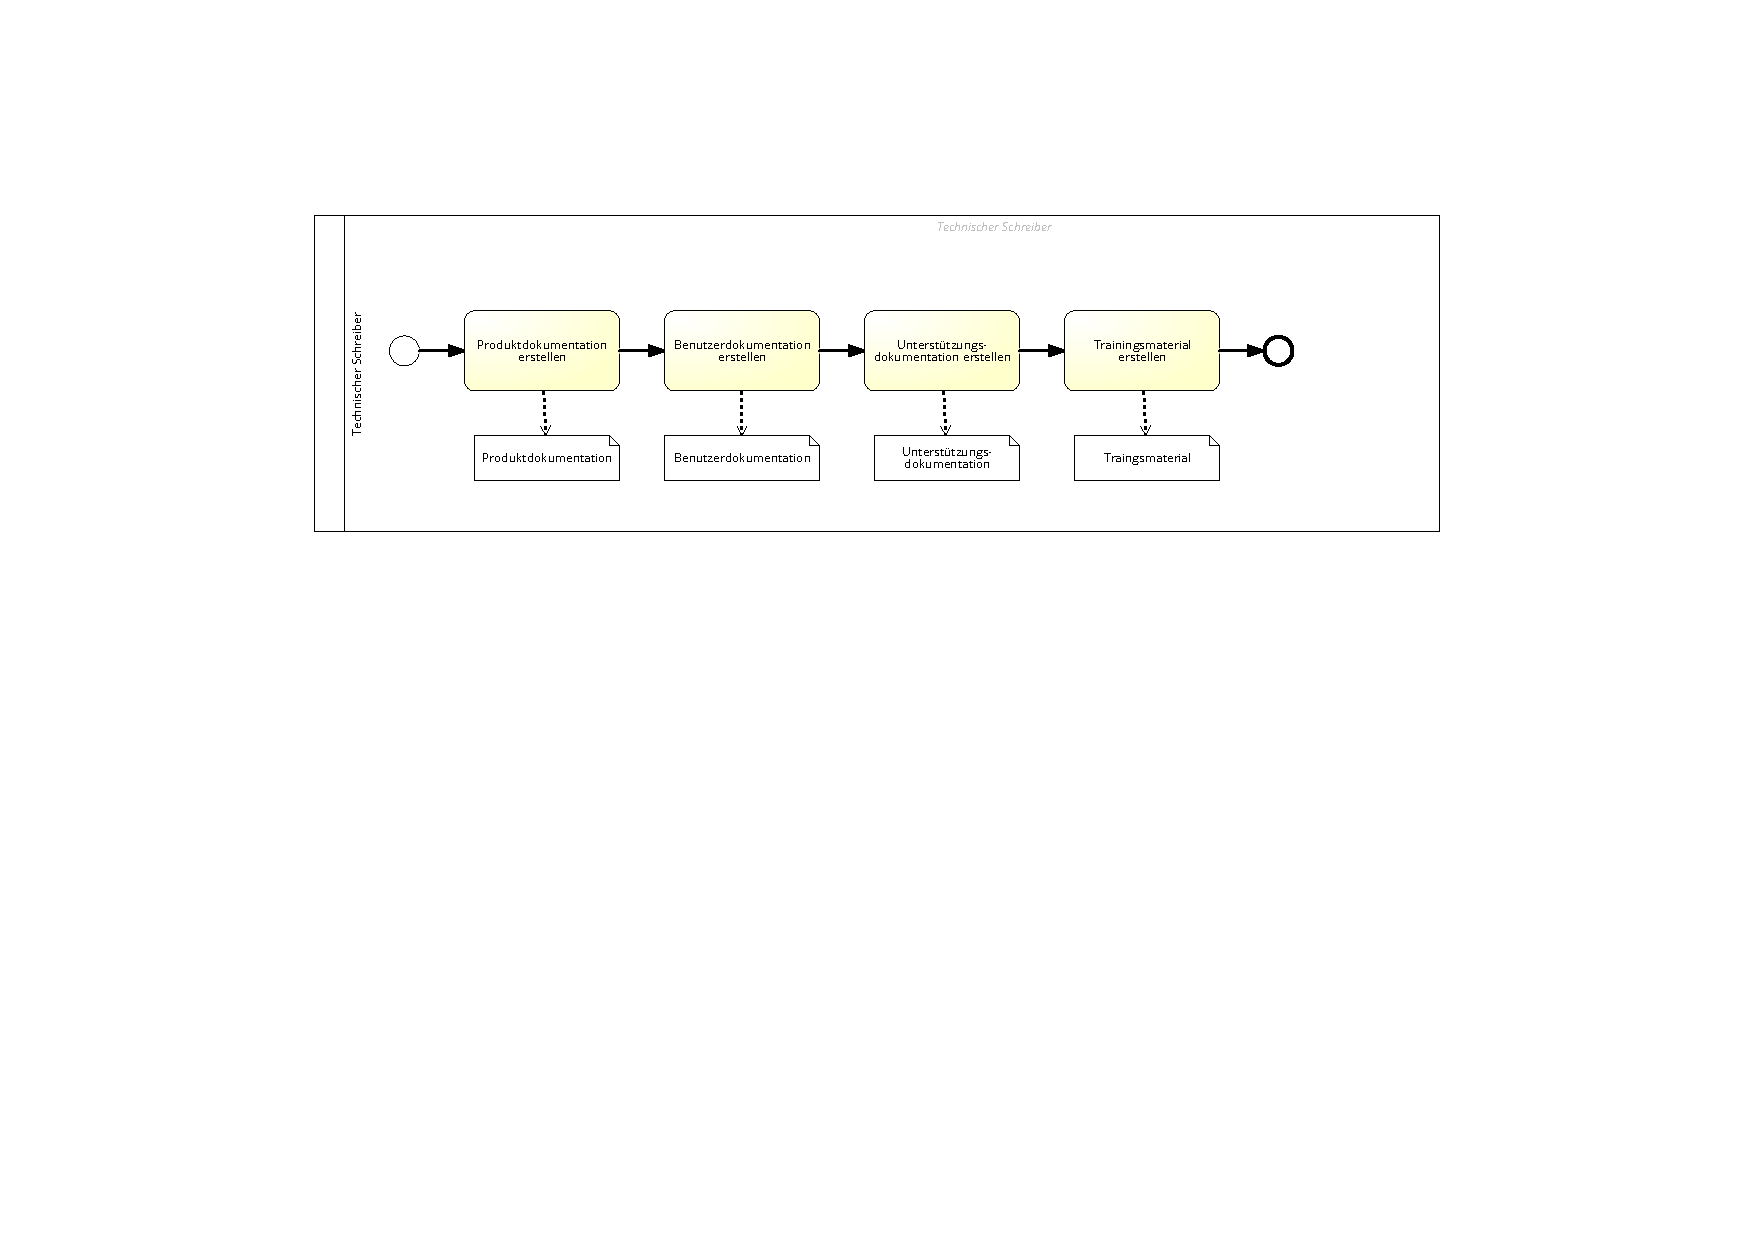
\includegraphics[width=\linewidth]{DevelopProductDocumentationKlein} %pdf, jpg, png...
  \caption{Produktdokumentation und Training erstellen - Construction}
  \label{fig:DevelopProductDocumentationKlein}
\end{center}
\end{figure}


\subsubsection{Release deployen-Transition}


Das Ergebnis dieses Unterprozesses ist die Release eines Sets von integrierten Komponenten in der Integrationsumgebung. \newline
Hierfür ist es notwendig ein komplettes, bereitstellungsfähiges Paket zu erstellen, welches vom Deployment Engineer in die Bereitstellungsumgebung releast werden kann.\newline
 Außerdem muss sichergestellt werden, dass der Roll-Out aus klaren, geprüften und wiederholbaren Anweisungen besteht und das Risiko eines Bereitstellungsfehlers muss minimiert werden. \newline
 Zudem muss sichergestellt werden, dass eine Release zu keinen ungewollten Unterbrechungen im Ablauf in der Produktionsumgebung führt. \newline
 Falls eine Release Probleme veursacht oder sie von den Stakeholdern als untauglich empfunden wird, muss diese Release von der Produktionsumgebung so schnell wie möglich entfernt werden. \newline
 Zusätzlich muss dafür gesorgt werden, dass Informationen über eine anstehende Release weitest möglich verteilt werden.\newline
 
  Abbildung \ref{fig:DeployReleaseTransitionKlein} zeigt die imperative Modellierung von \textit{Release deployen}.\newline
  Somit muss der Entwickler zunächst die \textit{Release zusammenstellen}, bevor der Deployment Engineer nacheinander die Aktivitäten \textit{Deploymentplan ausführen} und \textit{erfolgreiches Deployment sicherstellen} ausführt. Falls das Deployment erfolgreich ist, wird gleich anschließend die Aktivität \textit{Releasemitteilungen übermitteln} ausgeführt. Falls das Deployment nicht erfolgreich ist, muss zunächst die Aktivität \textit{Backoutplan ausführen} erledigt werden und erst danach die Aktivität \textit{Releasemitteilungen übermitteln} ausgeführt werden.


\begin{figure}[!htbp]
\begin{center}
  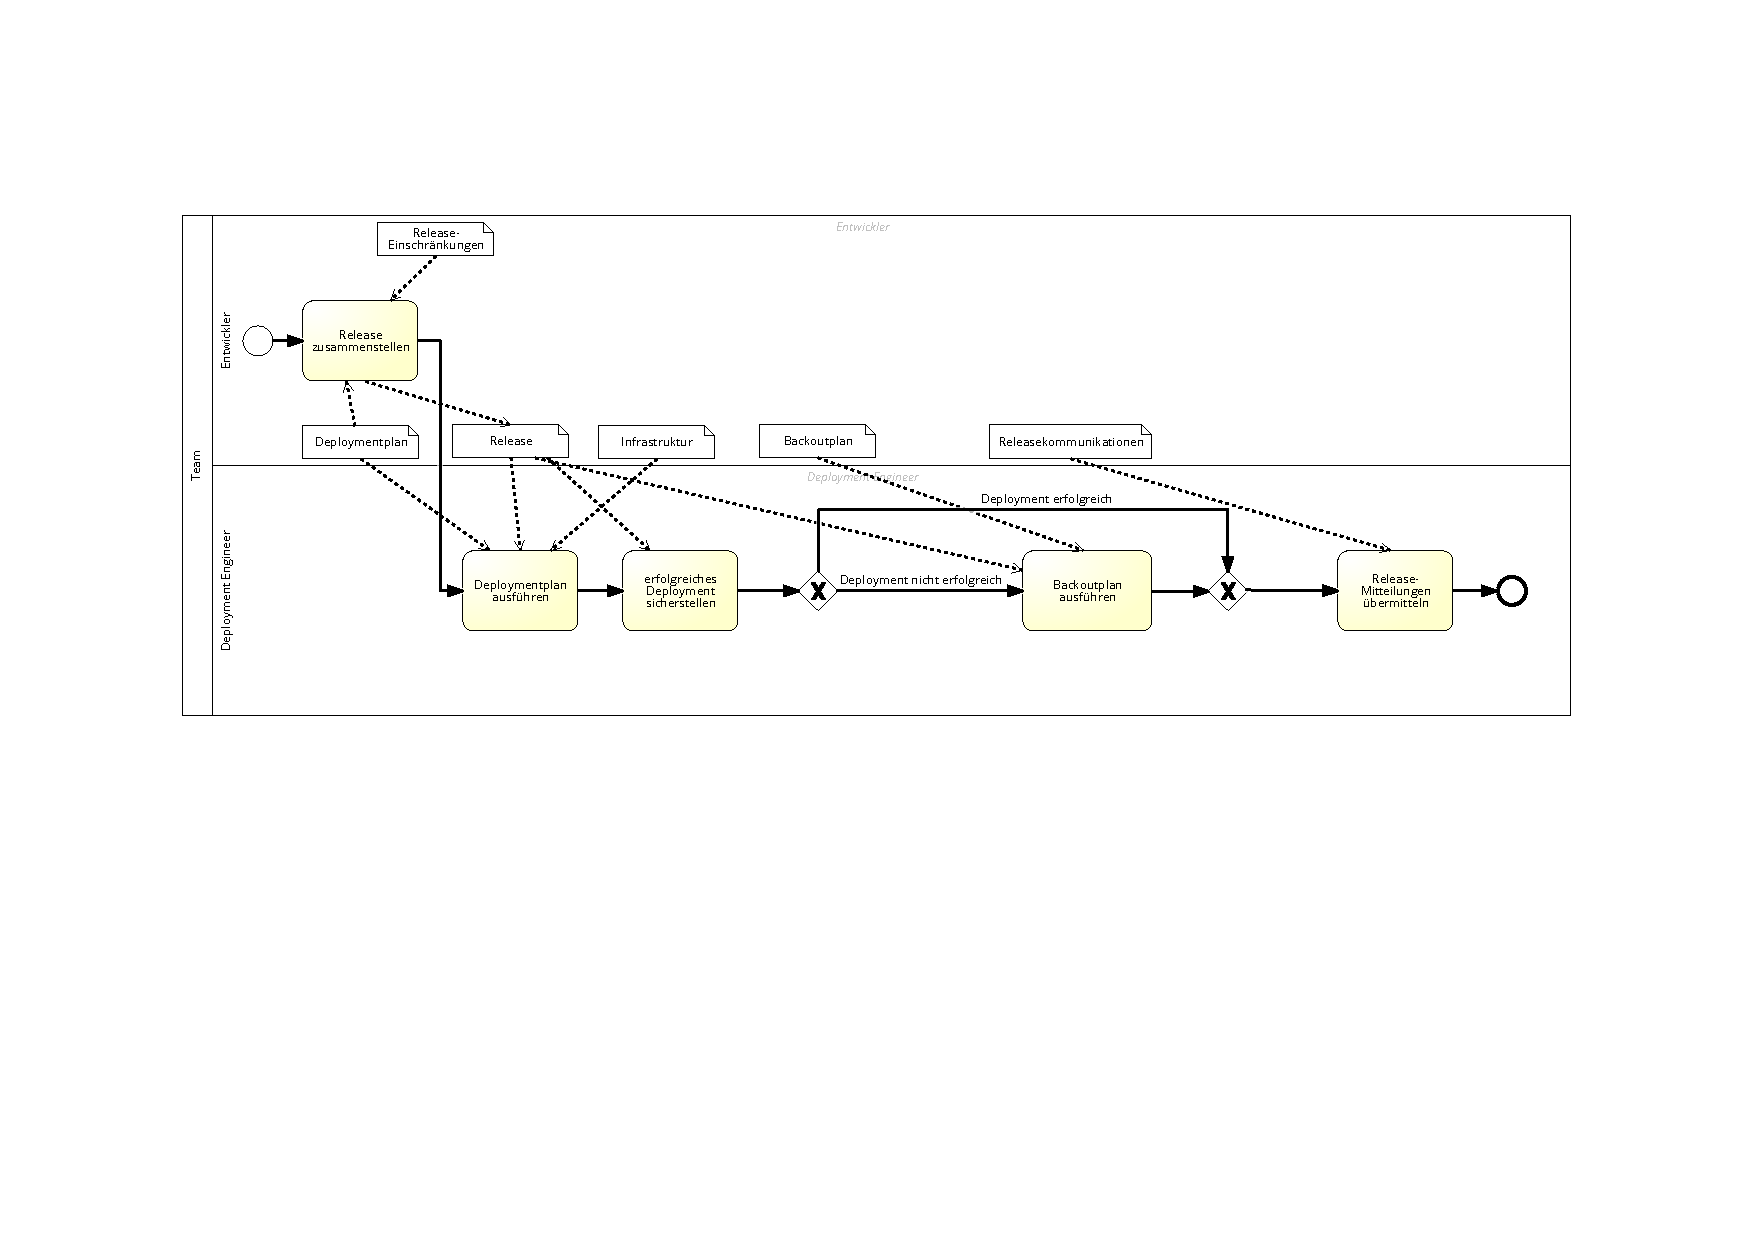
\includegraphics[width=\linewidth]{DeployReleaseTransitionKlein} %pdf, jpg, png...
  \caption{Release deployen-Transition}
  \label{fig:DeployReleaseTransitionKlein}
\end{center}
\end{figure}



\clearpage

\subsection{Deklarative Modellierung Open UP}




\subsubsection{Phasen des Open UP}


In Abbildung \ref{fig:OpenUpPhasenDec} sind die vier Phasen des Open UP deklarativ modelliert. Jede Phase kann in Iterationen mehrmals durchlaufen werden. Aus diesem Grund sind die vier Phasen durch das Constraint \textit{succesion} miteinander verbunden. Hierdurch wird gewährleistet, dass jede Phase so oft ausgeführt werden kann, wie nötig, aber das ebenfalls die Reihenfolge eingehalten wird. Z.B. kann die Phase Elaboration so erst durchlaufen werden, nachdem die Phase Inception durchlaufen wurde.
\begin{figure}[htp]
\begin{center}
  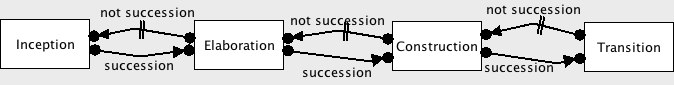
\includegraphics[width=\linewidth]{OpenUpPhasenDec} %pdf, jpg, png...
  \caption{Phasen Open UP- deklarativ}
  \label{fig:OpenUpPhasenDec}
\end{center}
\end{figure}




Abbildung \ref{fig:InceptionDecUnter} zeigt die deklarative Modellierung der Phase Inception. Die Aktivität \textit{Projekt planen und managen} kann parallel zu allen anderen Aktivitäten des Modells ausgeführt werden.\newline
Nach Ausführung der Aktivität \textit{Iteration planen} werden die Aktivitäten \textit{Anforderungen identifizieren und aufbereiten} und \textit{auf technisches Vorgehen einigen} parallel zueinander ausgeführt. Aus diesem Grund sind die Aktivitäten \textit{Anforderungen identifizieren und aufbereiten} und \textit{auf technisches Vorgehen einigen} mit der Aktivität  \textit{Projekt planen und managen} durch das Constraint succession verbunden, da sie erst nach deren Ausführung ausgeführt werden dürfen und auch ausgeführt werden müssen. \newline

\begin{figure}[htp]
\begin{center}
  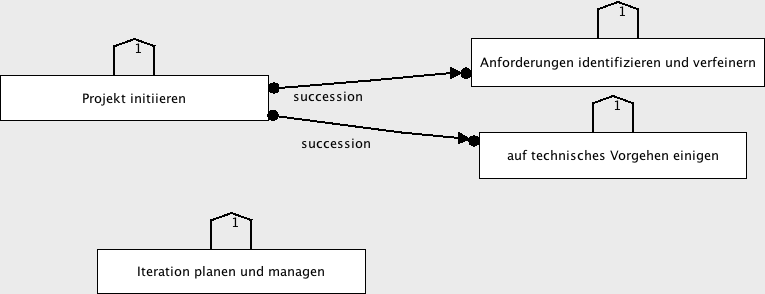
\includegraphics[width=\linewidth]{InceptionDecUnter} %pdf, jpg, png...
  \caption{Phasen Open UP Unterprozess Inception- deklarativ}
  \label{fig:InceptionDecUnter}
\end{center}
\end{figure}

In Abbildung \ref{fig:ElaborationDecUnter} ist die deklarative Modellierung der Phase Elaboration abgebildet. Die sechs Aktivtäten \textit{Anforderungen identifizieren und verfeinern, Architektur entwickeln, Lösungsinkrement entwickeln, Lösung testen, Iteration planen und managen} sowie \textit{weitere Aufgaben erledigen} werden parallel zueinander ausgeführt. Aus diesem Grund befindet sich lediglich das Constraint \textit{Ecactly 1} an jeder Aktivität, da sie innerhalb einer Prozessinstanz nur einmal ausgeführt werden dürfen, dies aber in beliebiger Reihenfolge. Im Falle einer weiteren Iteration der Phase Elaboration wird eine neue Prozessinstanz aufgerufen. \newline

\begin{figure}[htp]
\begin{center}
  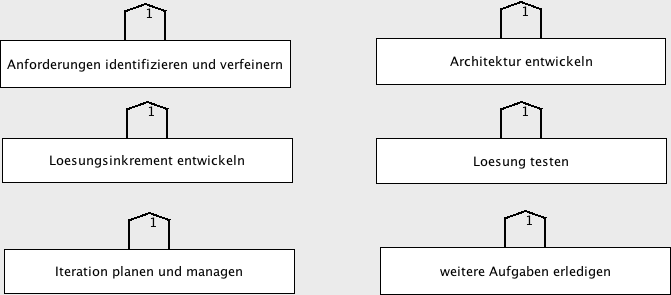
\includegraphics[width=\linewidth]{ElaborationDecUnter} %pdf, jpg, png...
  \caption{Phasen Open UP Unterprozess Elaboration- deklarativ} 
  \label{fig:ElaborationDecUnter}
\end{center}
\end{figure}

Die deklarative Modellierung der Phase Construction kann Abbildung \ref{fig:ConstructionDecUnter} entnommen werden. Hier werden die sechs Aktivitäten \textit{Anforderungen identifizieren und verfeinern, Lösungsinkrement entwickeln, Lösung testen, Iteration planen und managen, weitere Aufgaben erledigen} und \textit{Produktdokumentation und Training erstellen} nebeneinander parallel ausgeführt.
\begin{figure}[htp]
\begin{center}
  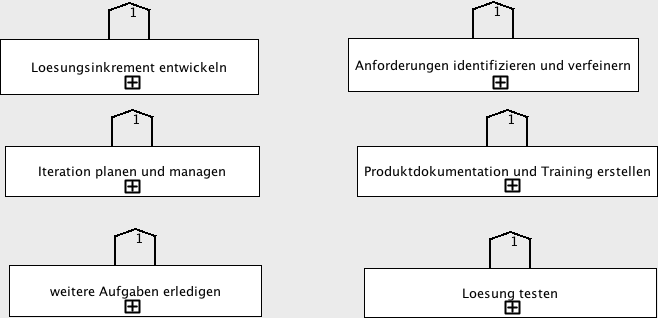
\includegraphics[width=\linewidth]{ConstructionDecUnter} %pdf, jpg, png...
  \caption{Phasen Open UP Unterprozess Construction- deklarativ}
  \label{fig:ConstructionDecUnter}
\end{center}
\end{figure}

Abbildung \ref{fig:TransitionDecUnter} kann die deklarative Modellierung der Phase Transition entnommen werden.\newline
Die Aktivitäten \textit{Anforderungen identifizieren und verfeinern, Produkt Training durchführen, Lösungsinkrement entwickeln, Lösung testen, Iteration planen und managen, weitere Aufgaben erledigen, Produktdokumentation und Training abschließen} sowie \textit{Release für die Produktion freigeben} werden parallel zueinander ausgeführt.

\begin{figure}[htp]
\begin{center}
  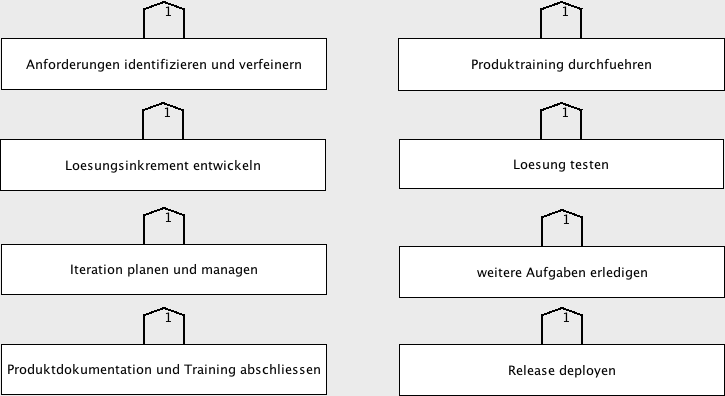
\includegraphics[width=\linewidth]{TransitionDecUnter} %pdf, jpg, png...
  \caption{Phasen Open UP Unterprozess Transition- deklarativ}
  \label{fig:TransitionDecUnter}
\end{center}
\end{figure}



Im weiteren Verlauf wird aus jeder der vier Phasen Inception, Elaboration, Construction und Transition des Open UP jeweils ein Unterprozess modelliert, da die Abbildung aller Unterprozesse aus jeder Phase den Rahmen der Arbeit sprengen würde. \newline
Somit wird für die Phase Inception der Unterprozess \textit{Iteration planen und managen}, für die Phase Elaboration der Unterprozess \textit{Anforderungen identifizieren und verfeinern}, für die Phase Construction der Unterprozess \textit{Release deployen} und für die Phase Transition der Unterprozess \textit{Produktdokumentation und Training erstellen} modelliert. Außerdem wird der in den drei Phasen Elaboration, Construction und Transition wiederkehrende Unterprozess \textit{Lösungsinkrement entwickeln} modelliert.


Die deklarative Modellierung von Develop Solution Increment kann Abbildung \ref{fig:Develop} entnommen werden.\newline
Falls eine \textit{Lösung designt} wird, muss danach der \textit{Entwicklertest implementiert} werden. Dies ist durch das Constraint \textit{chain response} zwischen diesen beiden Aktivitäten verlangt. Wenn der Entwicklertest implementiert wird, muss er danach auch ausgeführt werden und er kann nur ausgeführt werden, falls er vorher implementiert wurde (Constraints \textit{chain response} und \textit{precedence}).\newline
Bevor die Lösung implementiert werden kann, muss vorher der Entwicklertest ausgeführt werden (Constraint \textit{precedence}) und nach der Implementierung der Lösung muss nochmals der Entwicklertest ausgeführt werden (Constraint chain response).\newline
Vor dem \textit{Integrieren} muss der Entwicklertest ausgeführt worden sein, was durch das Constraint \textit{precedence} vorgegeben wird.
\begin{figure}[htp]
\begin{center}
  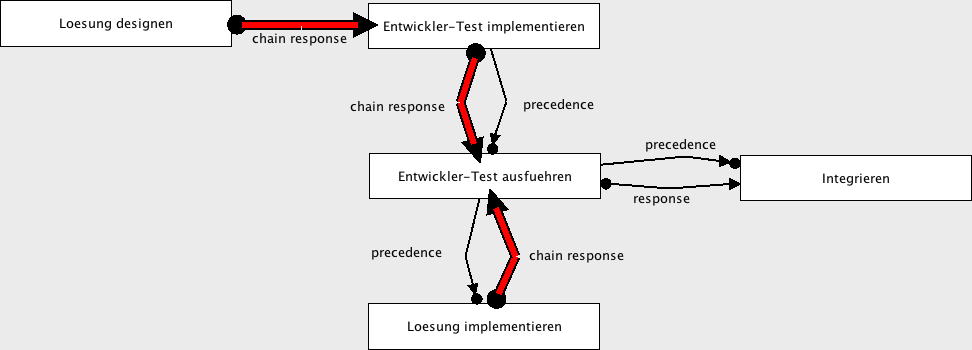
\includegraphics[width=\linewidth]{DevelopSolutionIncrement} %pdf, jpg, png...
  \caption{Lösungsinkrement entwickeln- deklarativ}
  \label{fig:Develop}
\end{center}
\end{figure}

Die deklarative Modellierung von Plan and manage iteration findet sich in Abbildung \textit{IterationPlanenDec}. Gestartet werden kann mit den Aktivitäten {Iteration planen} oder {Arbeitsaufgaben aussuchen}, da diese unabhängig voneinander ausgeführt werden können und von zwei verschiedenen Personen ausgeführt werden können.\newline
danach können entweder die Aktivitäten \textit{Umgebung vorbereiten} oder \textit{Arbeitsaufgaben in Entwicklungsaufgaben einteilen} ausgeführt werden. Diese sind jeweils mit ihrer Vorgängeraktivität durch das Constraint \textit{succession} verbunden und müssen deshalb auf die Ausführung ihres Vorgängers warten und nach dessen Ausführung ausgeführt werden.\newline
Das gleiche Ausführungsverhalten gilt auch für die anderen Aktivitäten im Prozess. 



\begin{figure}[htp]
\begin{center}
  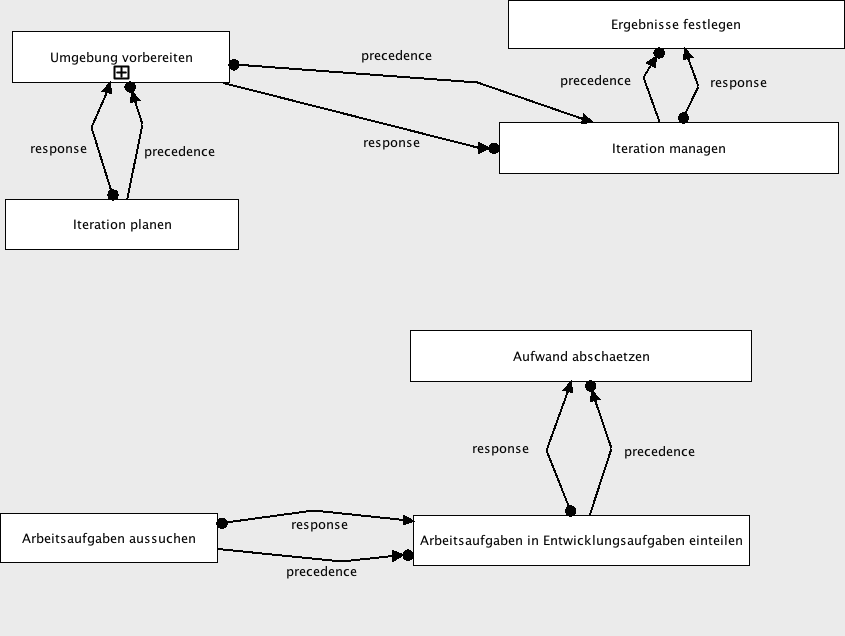
\includegraphics[width=\linewidth]{IterationPlanenDec} %pdf, jpg, png...
  \caption{Iteration planen und managen-Inception deklarativ}
  \label{fig:IterationPlanenDec}
\end{center}
\end{figure}

\begin{figure}[htp]
\begin{center}
  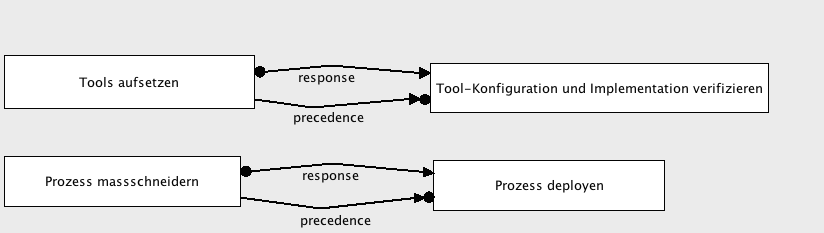
\includegraphics[width=\linewidth]{UmgebungvorbereitenDec} %pdf, jpg, png...
  \caption{Iteration planen und managen- Inception Unterprozess Umgebung vorbereiten- deklarativ}
  \label{fig:UmgebungVorbereitenDec}
\end{center}
\end{figure}


In Abbildung \ref{fig:IdentifyAndRefineDecKlein} ist die deklarative Modellierung von Identify and Refine Requirements dargestellt.\newline
Zu Beginn muss die Aktivität \textit{Anforderungen identifizieren und abgrenzen} ausgeführt werden, was durch das init-Label dargestellt ist. Im Anschluss muss die Aktivität \textit{Use-Case-Szenarien detaillieren} ausgeführt werden, was durch das Constraint \textit{chain response} festgelegt ist. Das Constraint \textit{precedence} legt hingegen fest, dass bevor \textit{Use-Case-Szenarien detaillieren} ausgeführt werden kann, zunächst \textit{Anforderungen identifizieren und abgrenzen}  bearbeitet werden muss. Die gleichen Constraints gelten zwischen \textit{Use-Case-Szenarien detaillieren} und \textit{Systemweite Anforderungen detaillieren} sowie zwischen \textit{Systemweite Anforderungen detaillieren} und \textit{Testfaelle erstellen}. Alle Aktivitäten werden genau einmal ausgeführt, was jeweils durch das 1-Label dargestellt ist. 

\begin{figure}[h]
\begin{center}
  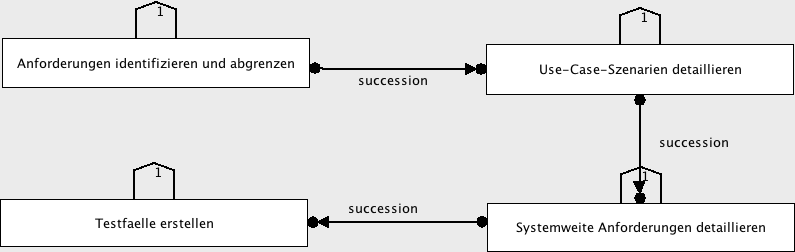
\includegraphics[width=\linewidth]{IdentifyAndRefineDecKlein} %pdf, jpg, png...
  \caption{Anforderungen identifizieren und verfeinern-Elaboration}
  \label{fig:IdentifyAndRefineDecKlein}
\end{center}
\end{figure}



Abbildung \ref{fig:DevelopProductDecKlein} zeigt die deklarative Modellierung von Develop Product Documentation.\newline
Zu Beginn muss die Aktivität \textit{Produktdokumentation entwickeln} ausgeführt werden, was durch das init-Label dargestellt ist. Im Anschluss muss die Aktivität \textit{Benutzerdokumentation entwickeln} ausgeführt werden. Dies ist durch das Constraint \textit{chain response} festgelegt ist. Das Constraint \textit{precedence} legt hingegen fest, dass bevor \textit{Benutzerdokumentation entwickeln} ausgeführt werden kann, zunächst \textit{Produktdokumentation entwickeln} bearbeitet werden muss. Die gleichen Constraints gelten zwischen \textit{Benutzerdokumentation entwickeln} und \textit{Unterstützungsdokumentation entwickeln} sowie zwischen \textit{Unterstützungsdokumentation entwickeln} und \textit{Trainingsmaterial entwickeln}. Alle Aktivitäten werden genau einmal ausgeführt, was jeweils durch das 1-Label dargestellt ist. 

\begin{figure}[htp]
\begin{center}
  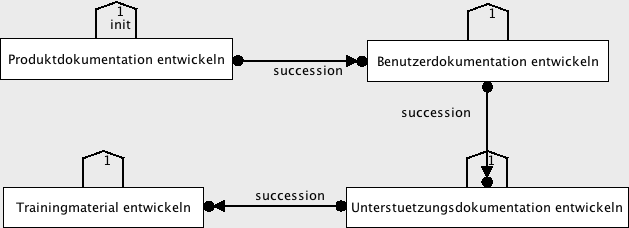
\includegraphics[scale=0.6]{DevelopProductDecKlein} %pdf, jpg, png...
  \caption{Produktdokumentation und Training erstellen-Construction}
  \label{fig:DevelopProductDecKlein}
\end{center}
\end{figure}

Abbildung \ref{fig:DeployReleaseDecKlein} zeigt die deklarative Modellierung von Deploy Release.\newline
Zu Beginn muss Die Aktivität \textit{Release zusammenstellen} bearbeitet werden, was durch das init-Constraint vorgegeben ist. Danach wird muss die Aktivität \textit{Deploymentplan ausfuehren} durchgeführt werden (Constraint response), aber erst nachdem \textit{Release zusammenstellen} durchgeführt wurde (Contsraint precedence).\newline
Die gleichen Constraints gelten zwischen den Aktivitäten \textit{Deploymentplan ausfuehren} und \textit{erfolgreiches Deployment sicherstellen}.\newline
Nach Abschluss der Aktivität \textit{erfolgreiches Deployment sicherstellen} kann entweder die Aktivität \textit{Backoutplan ausfuehren} ausgeführt werden, welche optinal ist (0..1 Constraint) oder die Aktivität \textit{Release-Mitteilungen uebermitteln}, welche auf jeden Fall ausgeführt werden muss.\newline 
Nach Ausführung von \textit{Release-Mitteilungen uebermitteln} darf \textit{Backoutplan ausfuehren} nicht mehr durchgeführt werden. Dies stellt das Constraint \textit{not succession} sicher.
\begin{figure}[htp]
\begin{center}
  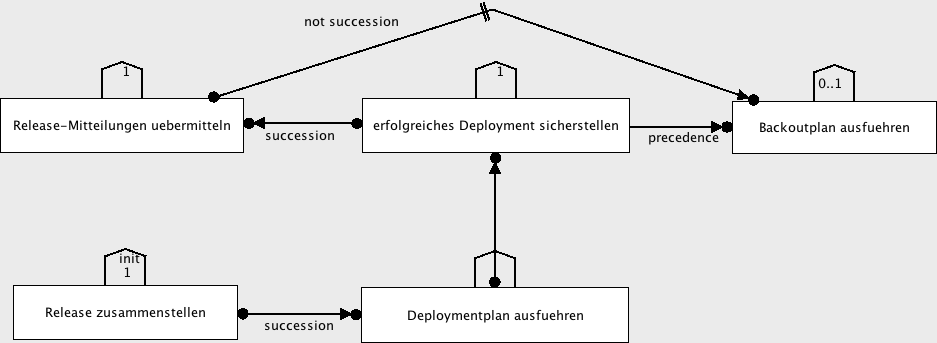
\includegraphics[width=\linewidth]{DeployReleaseDecKlein} %pdf, jpg, png...
  \caption{Release deployen-Transition}
  \label{fig:DeployReleaseDecKlein}
\end{center}
\end{figure}


\subsection{Vergleich}

Abbildung \ref{fig:PhasenOpenUpExcel} zeigt die Auswertung der Elemente im Modell Phasen des Open UP. Während bei BPMN vier Aktivitäten, acht Gateways (keine unterschiedlichen) und 17 Sequenzflusselemente, also gesamt 29 Elemente für das Modell benötigt werden, werden in ConDec nur vier Aktivitäten und sechs Constraints (zwei verschiedene), also insgesamt zehn Elemente verwendet.

\begin{figure}[htp]
\begin{center}
  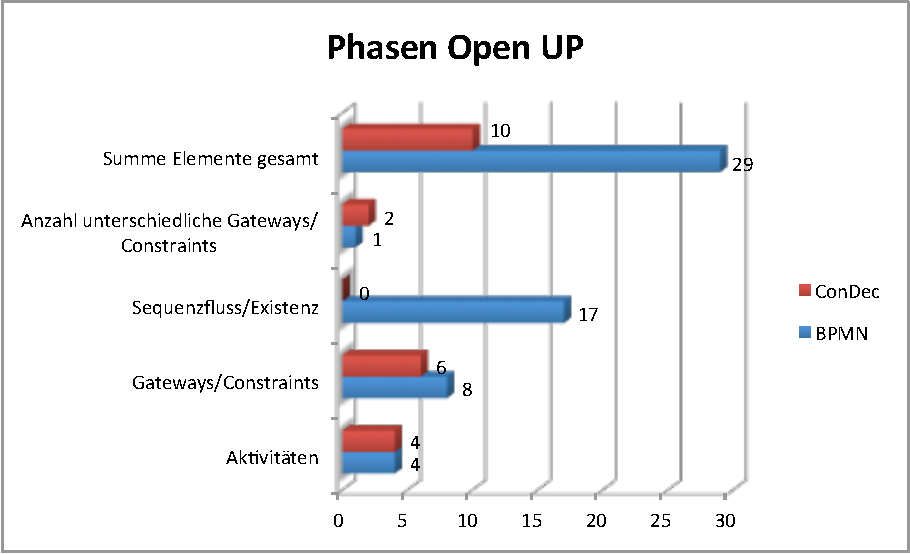
\includegraphics[scale=0.6]{PhasenOpenUpExcel} %pdf, jpg, png...
  \caption{Phasen Open UP}
  \label{fig:PhasenOpenUpExcel}
\end{center}
\end{figure}


\subsubsection {Phasen Open UP-Inception}

Die Anzahl der Elemente zur Darstellung der Phase Inception in ConDec und BPMN können Abbildung \ref{fig:InceptionExcel} entnommen werden. BPMN benötigt somit insgesamt 19 Elemente zur Darstellung dieser Phase (vier Aktivitäten, vier Gateways und 15 Verbindungselemente), ConDec nur zehn (vier Aktivitäten, sechs Constraints). Bei BPMN wird nur eine Sorte an Gateways verwendet und bei ConDec werden zwei unterschiedliche Constraints benötigt.\newline
\begin{figure}[htp]
\begin{center}
  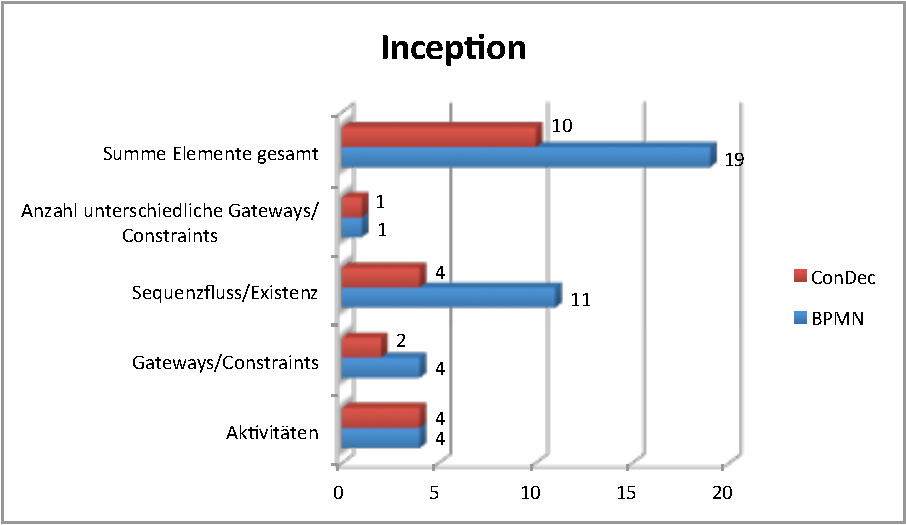
\includegraphics[scale=0.6]{InceptionExcel} %pdf, jpg, png...
  \caption{Open UP-Inception}
  \label{fig:InceptionExcel}
\end{center}
\end{figure}

Zur Darstellung der Phase Elaboration werden in BPMN insgesamt 22 Elemente und in ConDec 14 Elemente benötigt, wie Abbildung \ref{fig:ElaborationExcel} entnommen werden kann. Weiterhin werden jeweils sechs Aktivitäten in beiden Prozessmodellierungssprachen verwendet. In BPMN sind zwei Gateways (keine unterschiedlichen) und 14 Sequenzflusselemente, also insgesamt 16 Verbindungselemente notwendig. ConDec hingegen benötigt acht Existenz-Constraints. \newline

\begin{figure}[htp]
\begin{center}
  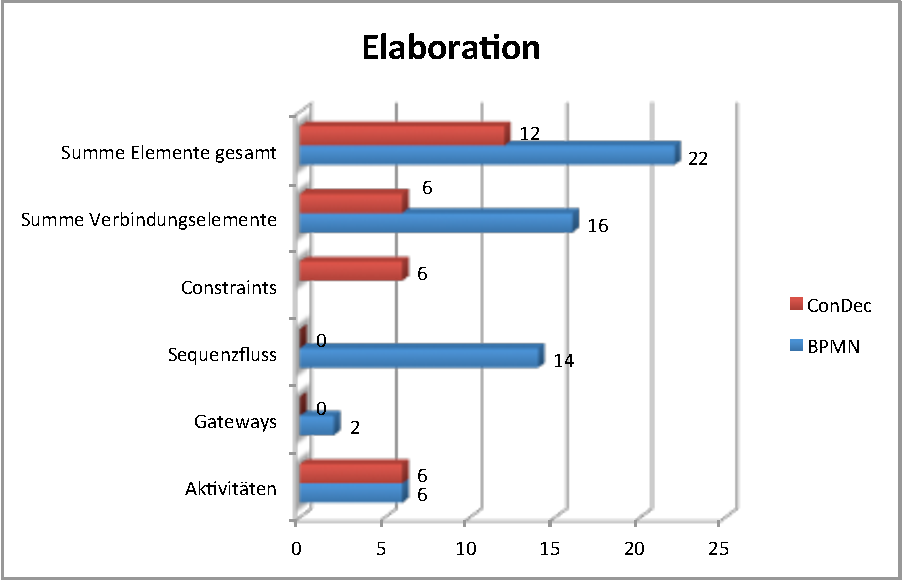
\includegraphics[scale=0.6]{ElaborationExcel} %pdf, jpg, png...
  \caption{Open UP-Elaboration}
  \label{fig:ElaborationExcel}
\end{center}
\end{figure}

Abbildung \ref{fig:ConstructionExcel} kann die Anzahl der Elemente zur Darstellung der Phase Construction entnommen werden. Demanch benötigt es in BPMN 24 Elemente und in ConDec 12 Elemente zur Darstellung des Prozesses. Sowohl in BPMN, als auch in ConDec werden jeweils sechs Aktivitäten benötigt. In BPMN sind vier Gateways (keine unterschiedlichen) und 14 Sequenzflusselemente erforderich. In ConDec werden sechs Existenz-Constraints zur darstellung des Ablaufes benötigt.\newline

\begin{figure}[htp]
\begin{center}
  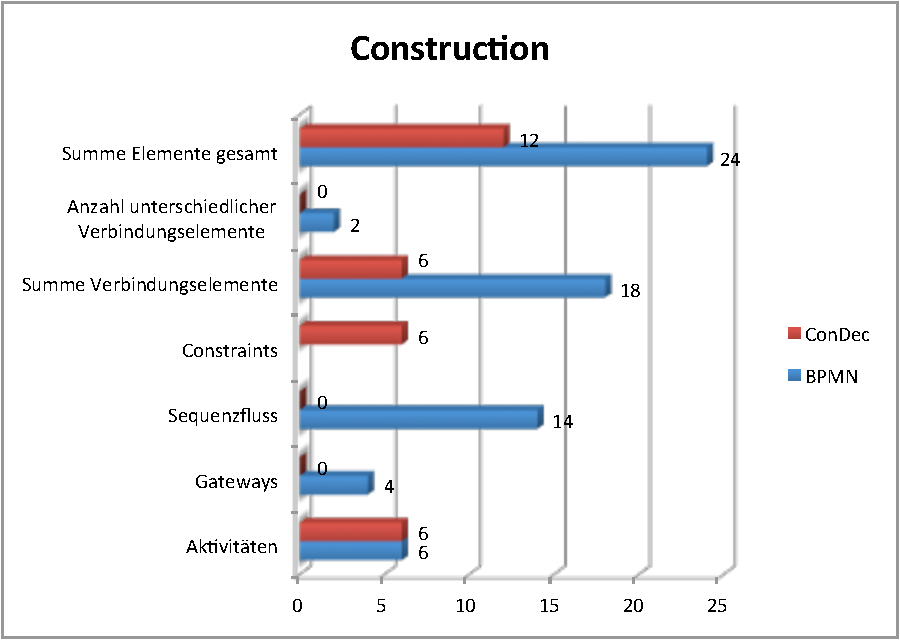
\includegraphics[scale=0.6]{ConstructionExcel} %pdf, jpg, png...
  \caption{Open UP-Construction}
  \label{fig:ConstructionExcel}
\end{center}
\end{figure}

Die Anzahl der notwendigen Elemente zur Darstellung der Phase Transition kann Abbildung \ref{fig:TransitionExcel} entnommen werden. Somit werden jeweils acht Aktivitäten verwendet. BPMN benötigt zwei Gateways (keine unterschiedlichen) und 18 Sequenzflusselemente zur korrekten Modellierung. In Condec braucht es insgesamt acht Existenz-Constraints zur Darstellung des Ablaufes.\newline

\begin{figure}[htp]
\begin{center}
  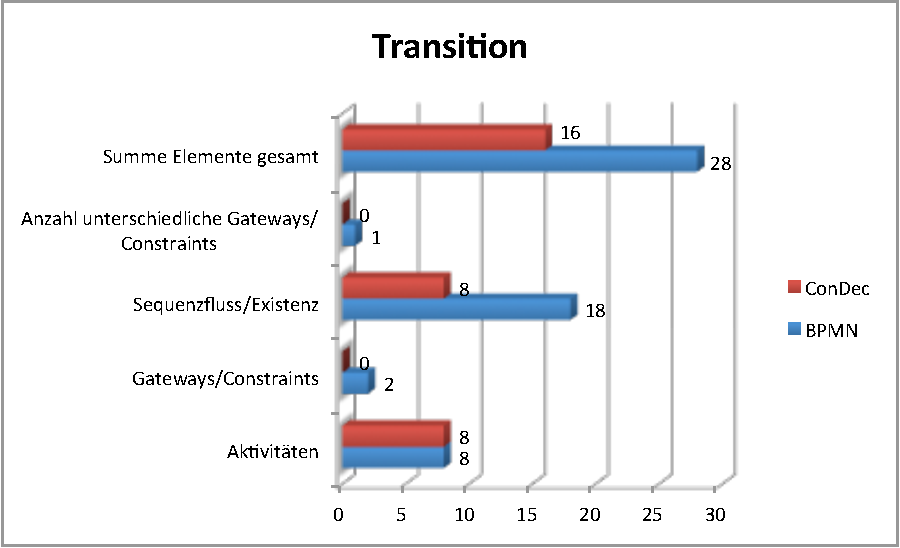
\includegraphics[scale=0.6]{TransitionExcel} %pdf, jpg, png...
  \caption{Open UP-Transition}
  \label{fig:TransitionExcel}
\end{center}
\end{figure}



Abbildung \ref{fig:IterationPlanenExcel} kann die Anzahl der Elemente, welche jeweils zur Darstellung des Unterprozesses Iteration planen und managen notwendig sind entnommen werden. Sowohl in BPMN, als auch in ConDec werden somit jeweils 11 Aktivitäten benötigt. In BPMN werden keine Gateways und 15 Sequenzflüsse verwendet. In ConDec sind zur korrekten Darstellung 21 Constraints notwendig. Somit werden in BPMN insgesamt 26 Elemente und in ConDec 32 Elemente verwendet.\newline

\begin{figure}[htp]
\begin{center}
  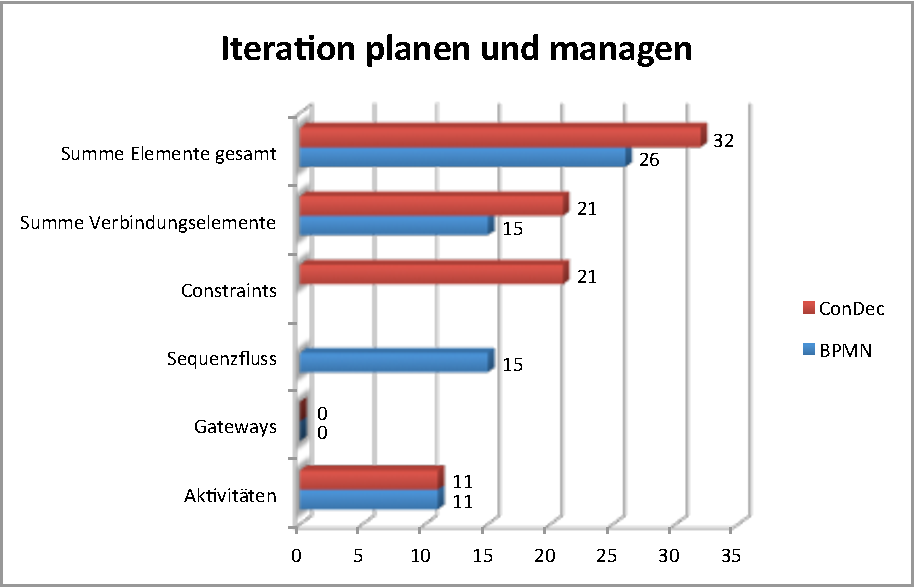
\includegraphics[scale=0.6]{IterationPlanenExcel} %pdf, jpg, png...
  \caption{Open UP-Iteration planen}
  \label{fig:IterationPlanenExcel}
\end{center}
\end{figure}

In Abbildung \ref{fig:AnforderungenIdentifizierenExcel} sind die Anzahl der Elemente zur Darstellung von Anforderungen identifizieren und verfeinern abgebildet. Demanch werden sowohl in BPMN, als auch in ConDec jeweils vier Akivitäten benötigt. Weiterhin sind keine Gateways und 5 Sequenzflusselemente in BPMN zur Darstellung nötig. In ConDec werden drei Constraints verwendet, aber keine unterschiedlichen. Insgesamt werden zur korrekten Abbildung des Metamodells in BPMN neun Elemente und in ConDec 11 Elemente benötigt.\newline

\begin{figure}[htp]
\begin{center}
  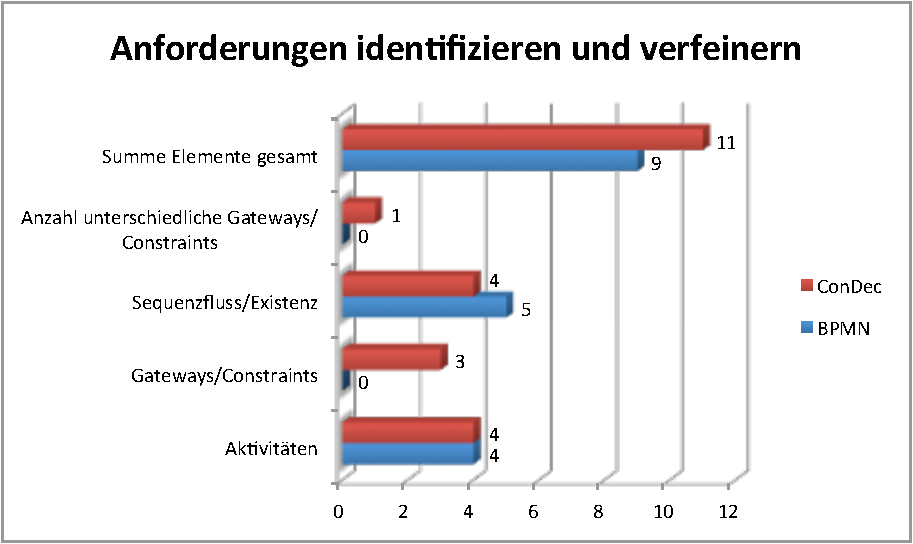
\includegraphics[scale=0.6]{AnforderungenIdentifizierenExcel} %pdf, jpg, png...
  \caption{Anforderungen identifizieren}
  \label{fig:AnforderungenIdentifizierenExcel}
\end{center}
\end{figure}

Die Anzahl der Elemente zur Darstellung des Prozesses Produktdokumentation entwickeln kann Abbildung \ref{fig:ProduktdokumentationExcel} entnommen werden. Es werden somit jeweils vier Aktivitäten zur Darstellung benötigt. Weiterhin werden in BPMN keine Gateways und sieben Sequenzflusselemente verwendet. In ConDec sind zur Darstellung sieben Constraints notwendig, jedoch keine unterschiedlichen Constraints. Insgesamt werden in BPMN neun Elemente und in ConDec 11 Elemente verwendet.\newline

\begin{figure}[htp]
\begin{center}
  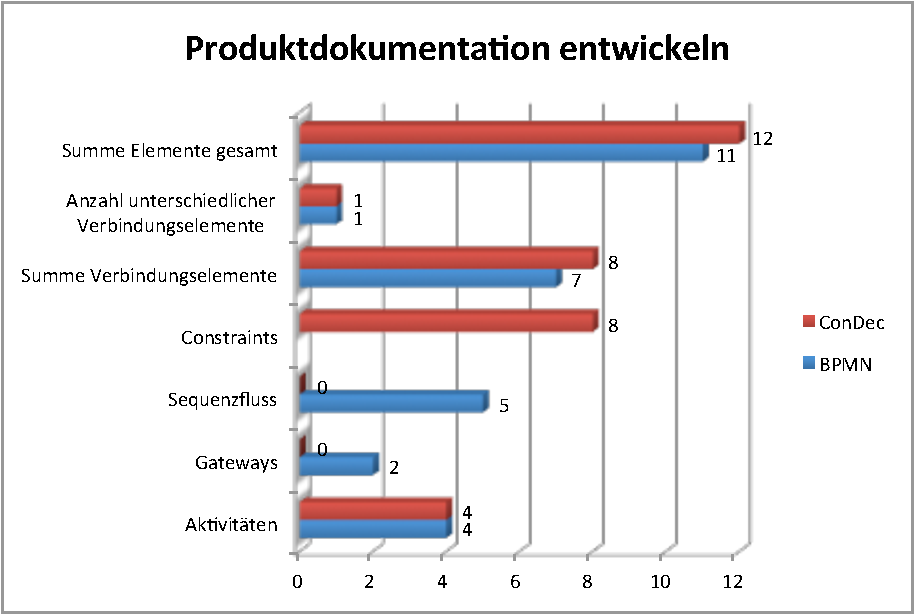
\includegraphics[scale=0.6]{ProduktdokumentationExcel} %pdf, jpg, png...
  \caption{Produktdokumentation erstellen}
  \label{fig:ProduktdokumentationExcel}
\end{center}
\end{figure}

Wie viele Elemente zur Modellierung des Prozesses Release deployen benötigt werden, ist in Abbildung \ref{fig:ReleaseDeployenExcel} aufgeführt. Jeweils fünf Aktivitäten werden in BPMN und ConDec verwendet. In BPMN sind zwei Gateways (keine verschiedene) und neun Sequenzflusselemente zur Darstellung des Ablaufes notwendig. In ConDec werden hierfür fünf Constraints (drei unterschiedliche)  und fünf Existenz-Constraints benötigt. Somit sind insgesamt 16 Elemente in BPMN und 15 Elemente in ConDec zur Darstellung notwendig. \newline
\begin{figure}[htp]
\begin{center}
  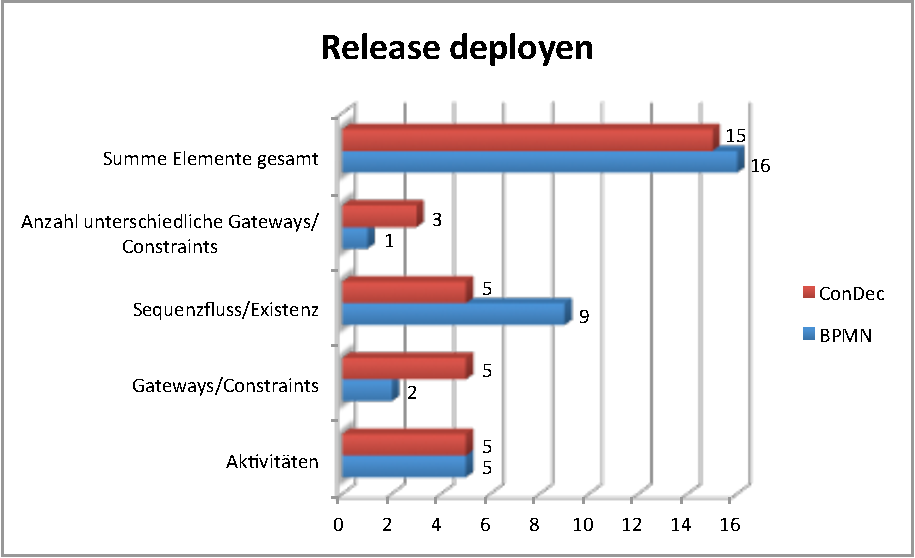
\includegraphics[scale=0.6]{ReleaseDeployenExcel} %pdf, jpg, png...
  \caption{Release deployen}
  \label{fig:ReleaseDeployenExcel}
\end{center}
\end{figure}

Bei dem Grundsatz der \textit{Richtigkeit} tritt bei ConDec wiederum das Problem auf, dass Rollen und Artefakte nicht darstellbar sind. Zwar ist dies bei den Phasen des Open UP kein Problem, da hier noch keine Rollen und Artefakte zugeordnet werden, jedoch bei den anderen Prozessen des Open UP (Iteration planen und managen, Anforderungen identifizieren und verfeinern, Produktdokumentation entwickeln und Release deployen). Da hier keine Rollen darstellbar sind, kann das jeweils im Metamodell enthaltene Verhalten in den ConDec-Modellen nicht vollständig wiedergegeben werden. Hierdurch leidet der Nutzen des Metamodells. \newline

Der Grundsatz des \textit{systematischen Aufbaus} kann wiederum nur von BPMN eingehalten werden, da ConDec keine Möglichkeit bietet, Artefakte ins Prozessmodell einzubinden.\newline

Die \textit{Relevanz} lässt sich bei beiden Prozessmodellierungssprachen gut einhalten, denn es ist weder bei einem in ConDec erstellten Modell, noch bei einem in BPMN erstellten Modell notwendig, weitere Informationen zur Erhöhung der Qualität des Modells hinzuzufügen.\newline

Die \textit{Wirtschaftlichkeit} lässt sich auch beim Open UP bei beiden Prozessmodellierungssprachen einhalten, da der Aufwand zur Erstellung der Modelle bei BPMN und ConDec gleich groß ist.\newline

In Bezug auf die \textit{Klarheit} fällt gerade bei Betrachtung der Modelle der Phasen Inception, Elaboration, Construction und Transition auf, das bei Modellen bei denen mehrere Aktivitäten parallel zueinnander ablaufen in BPMN deutlich mehr Elemente zur Darstellung des gleichen Sachverhaltes notwendig sind, als in ConDec. Bei allen vier Modellen sind doppelt so viele, teilweise auch mehr als doppelt so viele Elemene zur Darstellung in BPMN notwendig, als in ConDec. Dies liegt an der Anzahl der Verbindungselemente. BPMN weißt eine hohe Anzahl an eingehenden und ausgehenden Kanten an den parallelen Gateways auf. Da die Parallelität in ConDec nicht durch Constraints dargestellt werden muss, werden in ConDec nur die Existenz-Constraints benötigt, um die Aktivitäten auf einmalige Ausführung zu beschränken. Da sich die hohe Anzahl an Verbindungselementen in BPMN negativ auf die Verständlichkeit auswirken kann und in ConDec nur die leicht verständlichen Existenz-Constraints verwendet werden, sind die ConDec-Modelle die leichter verständlichen Modelle. \newline

Das Gleiche gilt für die Darstellung der Phasen des Open UP. Hier werden zur Darstellung des Prozesses in BPMN drei-mal so viele Elemente benötigt, wie in ConDec. Dies liegt hier an der hohen Anzahl der XOR-Gateways, die beim Modellieren des Prozesses notwendig sind. Somit ist auch hier das Modell, welches mit ConDec erstellt wurde das leichter verständliche. \newline
Im Prozess Iteartion planen und managen gibt es keine Verzweigungen. In ConDec werden sieben Constraints zur Darstellung verwendet. Die Anzahl der Elemente insgesamt ist bei beiden Modellen ungefähr gleich groß (ein Elemente mehr bei BPMN). Auf Grund der geringeren Komplexität des mit BPMN erstellten Modelles, da dort keine Gateways eingesetzt werden müssen, ist dieses das verständlichere.\newline
Bei den Prozessen Anforderungen identifizieren und verfeinern und Produktdokumentation entwickeln weißen die ConDec-Modelle eine leicht höhere Anzahl an Verbindungselementen und Elementen insgesamt auf. Außerdem werden hier auch in ConDec jeweils drei Constraints verwendet und in BPMN keine Gateways. Dies macht die ConDec-Modelle komplexer als die BPMN-Modelle, weswegen die mit BPMN erstellten Modelle verständlicher sind.\newline
Beim Prozess Release deployen werden fast gleich viele Elemente in ConDec, wie auch in BPMN zur Darstellung des Prozesses benötigt (ein Element mehr in BPMN). In ConDec werden insgesamt fünf Constraints und drei verschiedene zur Darstellung des Sachverhaltes benötigt, in BPMN nur zwei Gateways. Somit liegt hier das BPMN-Modell in Bezug auf die Komplexität unter dem ConDec-Modell und ist somit das verständlichere.\newline
Somit liegt ConDec bei der Darstellung der Phasen, in denen viele parallele Abläufe dargestellt werden bei der \textit{Klarheit} vorne, während bei den anderen Modellen es Schleifen oder keine Verzweigungen zum Darstellen gibt BPMN vorne liegt.\newline

Die Abläufe der Diagramme wurden in Signavio und Declare getestet und somit ist hier ihre \textit{Vergleichbarkeit} gewährleistet.\newline
Bei der Darstellung der Phasen des Open UP werden doppelt so viele Elemente in ConDec, wie in BPMN verwendet. Hier ist deshalb die \textit{Vergleichbarkeit} nicht ganz gewährleistet. Bei den anderen Modellen des Open UP unterscheidet sich die Anzahl der Elemente kaum voneinander, wodurch die Vergleichbarkeit hier gewährleistet ist. \newline
Bei ConDec muss wieder auf die Darstellung von Artefakten und Rollen verzichtet werden, wodurch die \textit{Vergleichbarkeit} der Modelle von ConDec behindert wird. Somit weiden hier beide Prozessmodellierungssprachen Stärken und Schwächen auf.\newline

Eine Zusammenfassung, welche Modellierungssprache bei welchem Grundsatz ehr überzeugt hat, kann Abbildung \ref{fig:TabelleOpenUP} entnommen werden. \newline


\begin{figure}[htp]
\begin{center}
  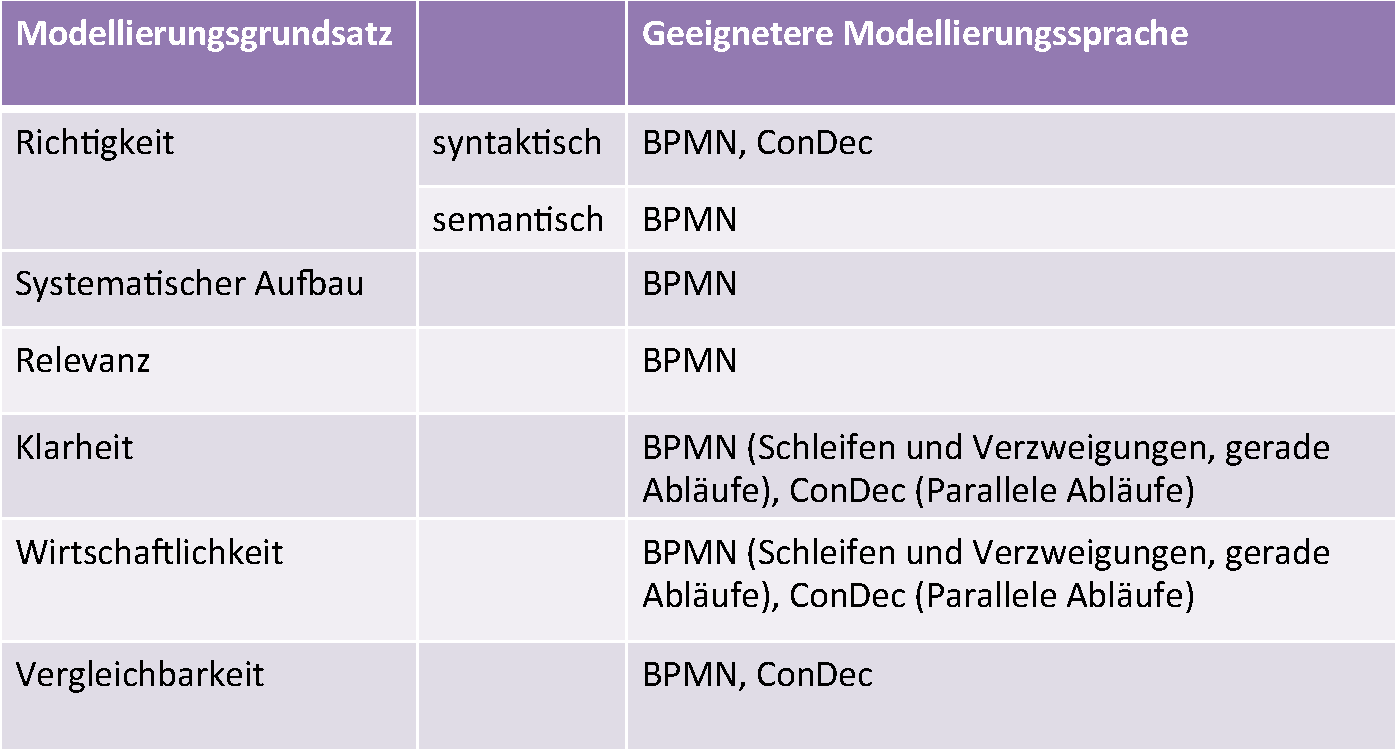
\includegraphics[scale=0.6]{TabelleOpenUP} %pdf, jpg, png...
  \caption{Übersicht Vergleich Open UP}
  \label{fig:TabelleOpenUP}
\end{center}
\end{figure}


\section{V-Modell XT}


Das V-Modell XT zählt zu den schwergewichtigen Prozessmodellen \cite{Hanser2010}. Es wird als Entwicklungsstandard für die Durchführung von IT-Vorhaben in der öffentlichen Verwaltung in Deutschland herangezogen \cite{Kuhrmann2011}. Beschrieben werden im V-Modell XT die Abläufe im Verlauf eines Entwicklungsprojektes über Produkte, Rollen und Aktivitäten \cite{Friedrich2008}. Es wird somit ganz genau geregelt, \textit{Wer}, \textit{Wann}, \textit{Was} in einem Projekt zu tun hat \cite{2004vmodell}. Die Vorgehensbausteine ermöglichen neben einer Modularisierung der Abläufe auch eine flexible Zusammenstellung, wodurch das V-Modell XT auf die jeweils eigene Situation angepasst werden kann. \cite{Friedrich2008,Zoerner2012}. \newline
\subsection{Analyse V-Modell XT}

Abbildung \ref{fig:grundstruktur} zeigt die Grundstruktur des V-Modell XT, welche im Folgenden detailliert erläutert wird.
\begin{figure}[htp]
\begin{center}
  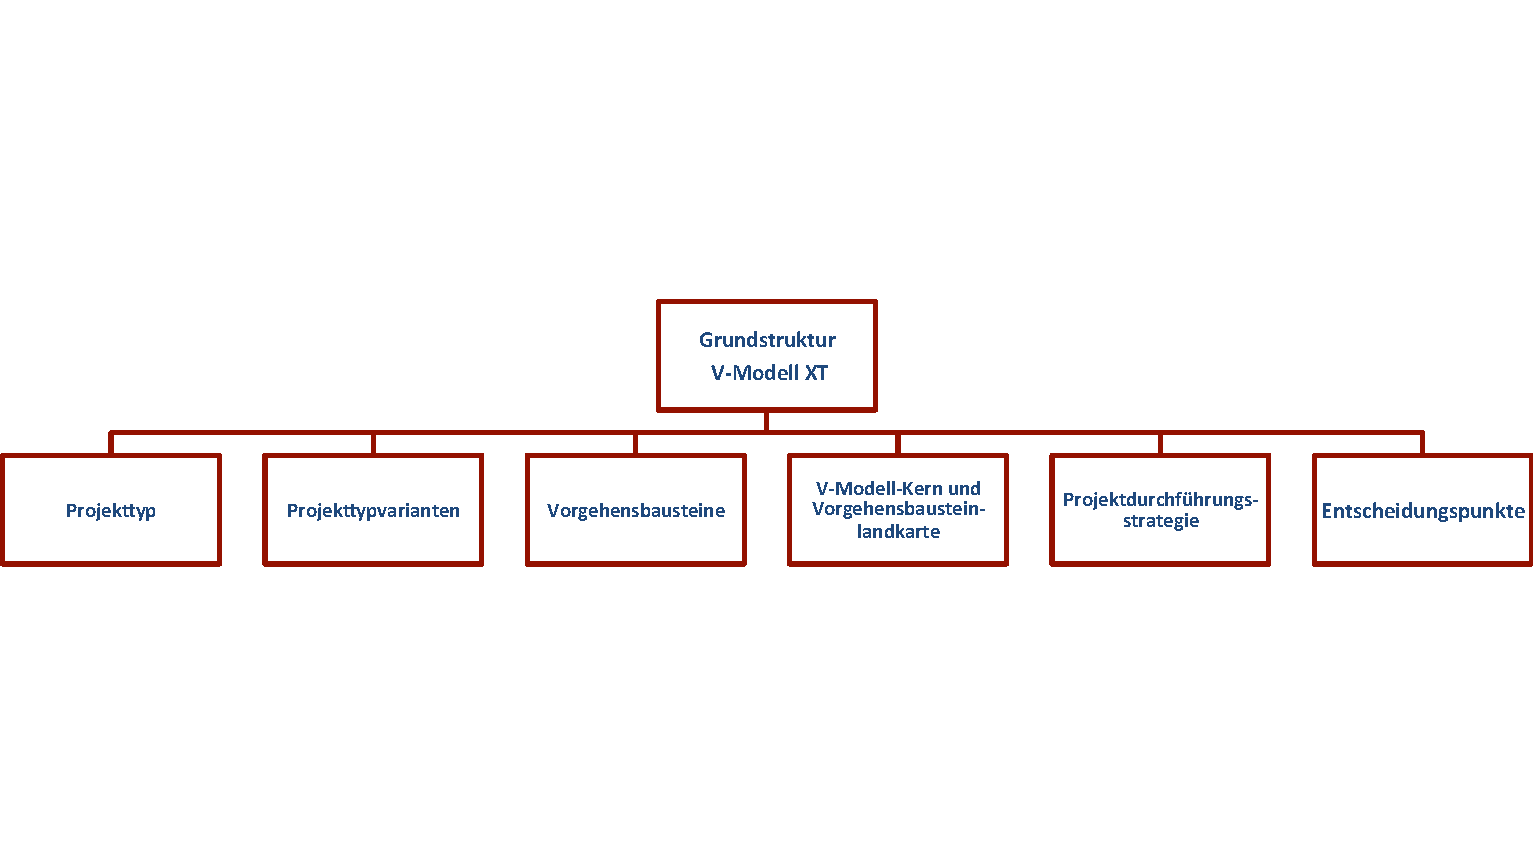
\includegraphics[width=\linewidth]{grundstruktur} %pdf, jpg, png...
  \caption{Grundstruktur V-Modell XT nach \cite{2004vmodell}}
  \label{fig:grundstruktur}
\end{center}
\end{figure}

\subsubsection{Projekttypen}
Nicht alle V-Modell-Projekttypen laufen nach exakt demselben Schema ab. Auf Grund ihrer charakteristischen Eigenschaften lassen sie sich demnach in unterschiedliche Projekttypen einteilen. Abbildung \ref{fig:Projekttypen} gibt einen ersten Überblick über die verschiedenen Projekttypen im V-Modell XT \cite{2004vmodell}.

\begin{figure}[htp]
\begin{center}
  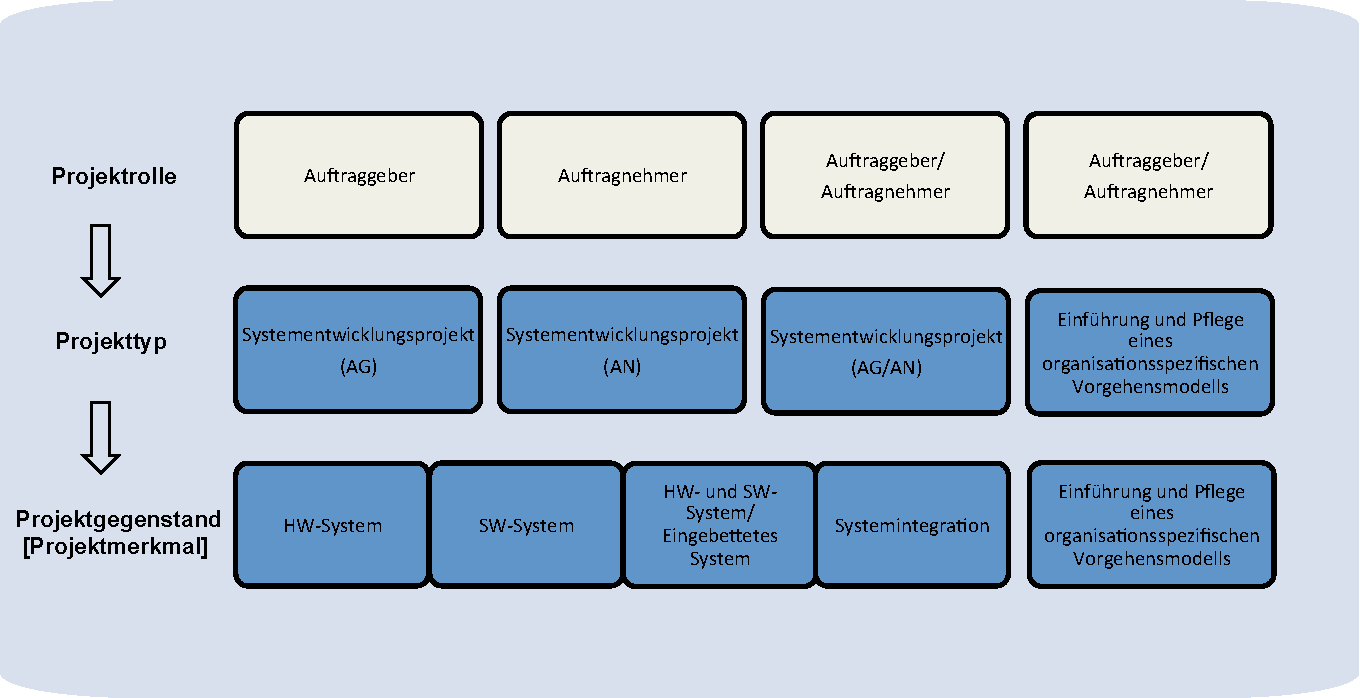
\includegraphics[width=\linewidth]{v-modell-rollen} %pdf, jpg, png...
  \caption{Projekttypen V-Modell XT nach \cite{2004vmodell}}
  \label{fig:Projekttypen}
\end{center}
\end{figure}

Es existieren somit vier verschiedene Projekttypen: \textit{Systementwicklungsprojekt eines Auftraggebers}, \textit{Systementwicklungsprojekt eines Auftragnehmers},  \textit{Systementwicklungsprojekt eines Augtraggebers/Auftragnehmers}  und \textit{Einführung und Pflege eines organisationsspezifischen Vorgehensmodells} \cite{reinhard2008}. \newline

Es werden drei verschiedene Projektrollen unterschieden, welche dem jeweiligen Projekttyp entsprechen: In der Rolle \textit{Auftragnehmer} wird ein vom \textit{Auftraggeber} spezifiziertes System entwickelt. Die Systementwicklung wird an einen oder mehrere \textit{Arbeitnehmer} weiter gegeben, wenn man sich in der Rolle \textit{Arbeitgeber} befindet. Das System  wird selbst entwickelt in der Rolle \textit{Auftraggeber/Auftragnehmer} \cite{brack2010,2004vmodell}.\newline


Beim \textit{Systementwicklungsprojekt eines Auftraggebers} wird die Entwicklung des Projektgegenstandes im Projektverlauf  ausgeschrieben und der Auftragnehmer trifft eine Auswahl anhand der eingehenden Angebote. Der Auftragnehmer, welcher für die Entwicklung des Projektgegenstandes ausgewählt wurde, entwickelt den Projektgegenstand, welcher dann vom Auftragnehmer abgenommen wird \cite{reinhard2008,2004vmodell}.\newline
Umgekehrt wird beim \textit{Systementwicklungsprojekt eines Auftragnehmers} im Laufe des Projektes ein Angebot erstellt und bei Auswahl durch den Auftraggeber ein Projektgegenstand entwickelt, welcher abschließend an den Auftraggeber ausgeliefert und von diesem abgenommen wird \cite{reinhard2008,2004vmodell}.\newline
Bei \textit{Einführung und Pflege eines organisationsspezifischen Vorgehensmodells} geht es um Projekte, welche Prozessmodelle z.B. das V-Modell einführen und verbessern wollen. Für diesen Zweck ist eine Analyse des vorherigen Prozessmodelles notwendig und etwaige Verbesserungsmöglichkeiten sind zu erfassen und durchzuführen \cite{reinhard2008,2004vmodell}.\newline
Wie aus Abbildung \ref{fig:Projekttypen} ersichtlich ist, kann es sich im V-Modell XT beim Projektgegenstand um ein Hardware (HW)-System, ein Software (SW)-System, ein eingebettetes System oder eine Systemintegration handeln \cite{brack2010,2004vmodell}. \newline

\subsubsection{Projekttypvarianten}
Für jeden der Projekttypen, gibt es im V-Modell XT mindestens eine passende Projekttypvariante. Diese bestimmt die Rahmenbedingungen für mögliche Abläufe eines Projektes. In Abbildung \ref{fig:Projekttypvarianten} sind die verschiedenen Projekttypvarianten des V-Modell XT aufgelistet und es wird gezeigt, mit welchen Merkmalen die zugehörigen Projekttypvarianten ausgewählt werden können \cite{2004vmodell}.   
\begin{figure}[htp]
\begin{center}
  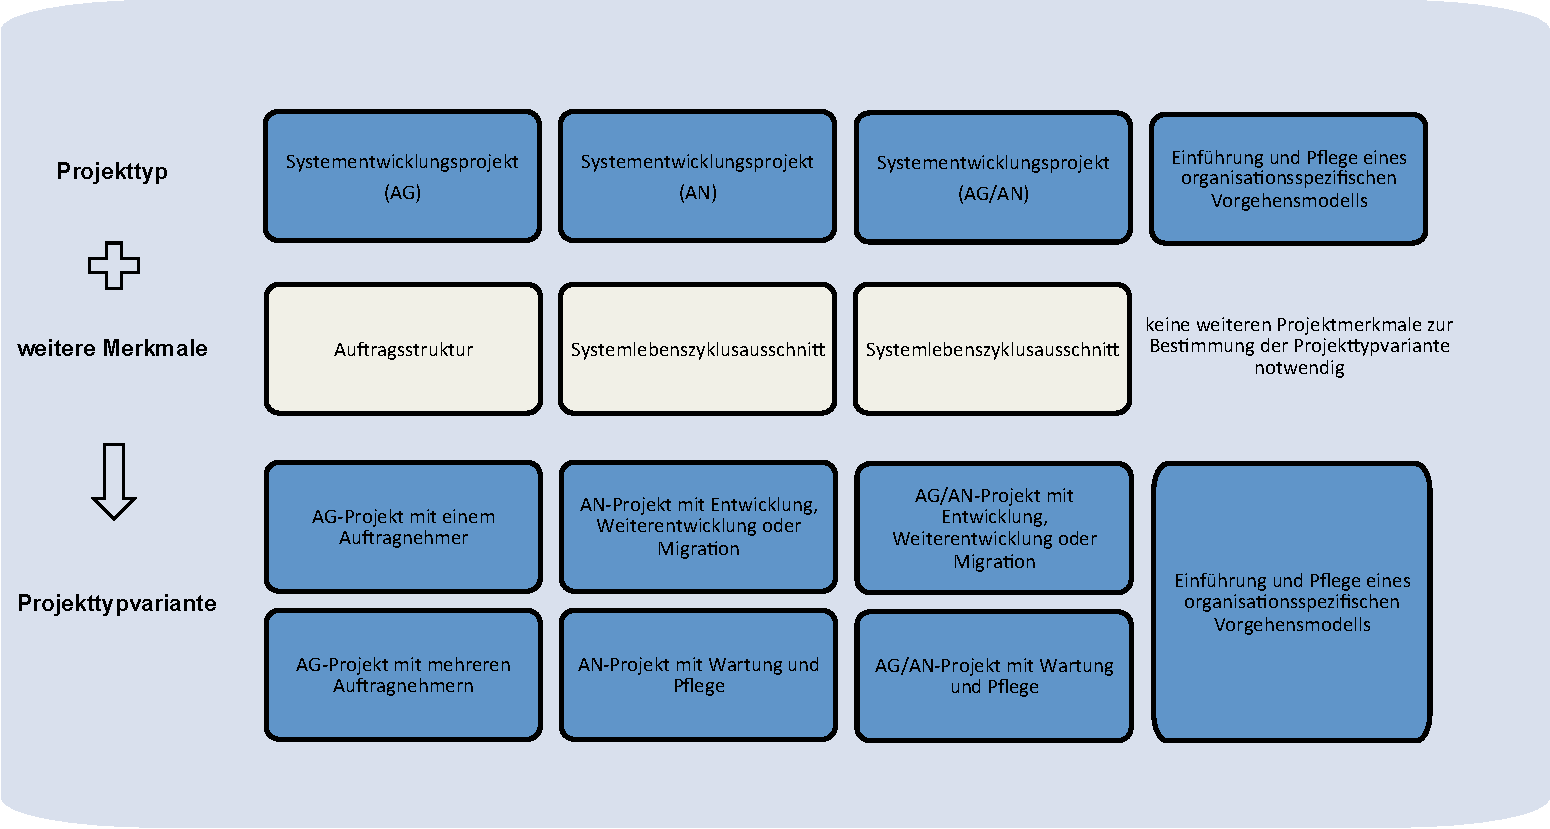
\includegraphics[width=\linewidth]{Projekttypvarianten-v-modell} %pdf, jpg, png...
  \caption{Zuordnung der Projekttypvarianten zu den Projekttypen des V-Modell XT \cite{2004vmodell}}
  \label{fig:Projekttypvarianten}
\end{center}
\end{figure}

Für den Projekttyp \textit{Systementwicklungsprojekt (AG)} existieren zwei verschiedene Projekttypvarianten, welche je nach \textit{Auftragsstruktur} ausgewählt werden. Falls der Auftraggeber mit nur einem Auftragnehmer zusammen arbeitet, ergibt sich die Projekttypvariante \textit{Systementwicklungsprojekt (AG)- Projekt mit einem Auftragnehmer}. Arbeitet der Auftraggeber mit mehreren Auftragnehmern zusammen, ergibt sich die Projekttypvariante \textit{Systementwicklungsprojekt (AG)- Projekt mit mehreren Auftragnehmern} \cite{2004vmodell}.\newline
Bei den Projekttypen \textit{Systementwicklungsprojekt (AN)} und \textit{Systementwicklungsprojekt (AG/AN)} wird die Unterscheidung anhand des Systemlebenszyklusausschnitt des Projektes durchgeführt. Somit wird in den Systemlebenszyklusausschnitten Entwicklung, Weiterentwicklung und Migration eine andere Projekttypvariante gewählt, als in Wartung und Pflege \cite{2004vmodell}.\newline 
Für den Projekttyp \textit{Einführung und Pflege eines organisationsspezifischen Vorgehensmodells} eyistiert nur eine einzige Projekttypvariante, weshalb hier keine weiteren Merkmale zur Bestimmung der Projekttypvariante notwendig sind \cite{2004vmodell}.\newline

  
 \subsubsection{Vorgehensbausteine}
Modulare, aufeinander aufbauende Vorgehensbausteine bilden den Kern des V-Modell XT. Vorgehensbausteine sind selbständig entwickelbare und änderbare Einheiten und bestehen aus Aktivitäten, Produkten und Rollen. Sie geben einerseits vor, \grqq Was\grqq{}  in einem Projekt zu tun ist, also welche Produkte zu erstellen sind und andererseits \grqq Wer\grqq, also welche konkrete Rolle für das jeweilige Produkt verantwortlich ist. Abbildung \ref{fig:vorgehensbausteine} gibt einen Überblick über diese \cite{ruf2008, 2004vmodell}.\newline

\begin{figure}[htp]
\begin{center}
  \includegraphics[width=\linewidth]{vorgehensbaustein} %pdf, jpg, png...
  \caption{Vorgehensbausteine V-Modell XT nach \cite{2004vmodell}}
  \label{fig:vorgehensbausteine}
\end{center}
\end{figure}

Ergebnisse und Zwischenergebnisse werden Produkte genannt. Komplexe Produkte können in ein oder mehrere Themen gegliedert werden und inhaltlich zusammengehörende Produkte können zu einer Disziplin zusammengefasst werden. Produkte können hierbei auch voneinander abhängig sein, sowohl innerhalb eines Vorgehensbausteins, als auch zwischen verschiedenen Vorgehensbausteinen \cite{2004vmodell}.\newline
Jedes Produkt wird von genau einer Aktivität fertig gestellt. Aktivitäten legen auch fest, wie die einzelnen Produkte zu bearbeiten sind. Sie bestehen aus einer oder mehreren Teilaktivitäten, sogenannten Arbeitsschritten. Diese stellen eine Art Arbeitsanleitung dar und bearbeiten eine oder mehrere Themen \cite{2004vmodell}.\newline
Durch Rollen werden eine Menge von Aufgaben und Verantwortlichkeiten gekapselt, wodurch das V-Modell XT unabhängig von organisatorischen Rahmenbedingungen bleibt. Eine Zuordnung von Personen, bzw. Organisationseinheiten zu einer Rolle erfolgt erst zu Beginn eines Projektes. Es wird jedem Produkt genau eine Rolle als Verantwortlicher zugewiesen, weitere Rollen können am Produkt als Mitwirkende mitarbeiten \cite{2004vmodell}. \newline



\subsubsection{V-Modell-Kern und Vorgehensbausteinlandkarte}

Um ein spezifisches Projekt an ein V-Modell-Projekt anzupassen, ist für jeden Projekttyp und jede Projekttypvariante genau vorgegeben, welche Vorgehensbausteine jeweils anzuwenden sind \cite{2004vmodell}. Hierdurch kann also ein individuelles V-Modell für ein Projekt erstellt werden \cite{heinrich2007}. Hierfür ist es notwendig, die Vorgehensbausteine für ein V-Modell-Projekt nach den Vorgaben des Projekttyps auszuwählen und festzulegen \cite{2004vmodell}. \newline

\begin{figure}[htp]
\begin{center}
  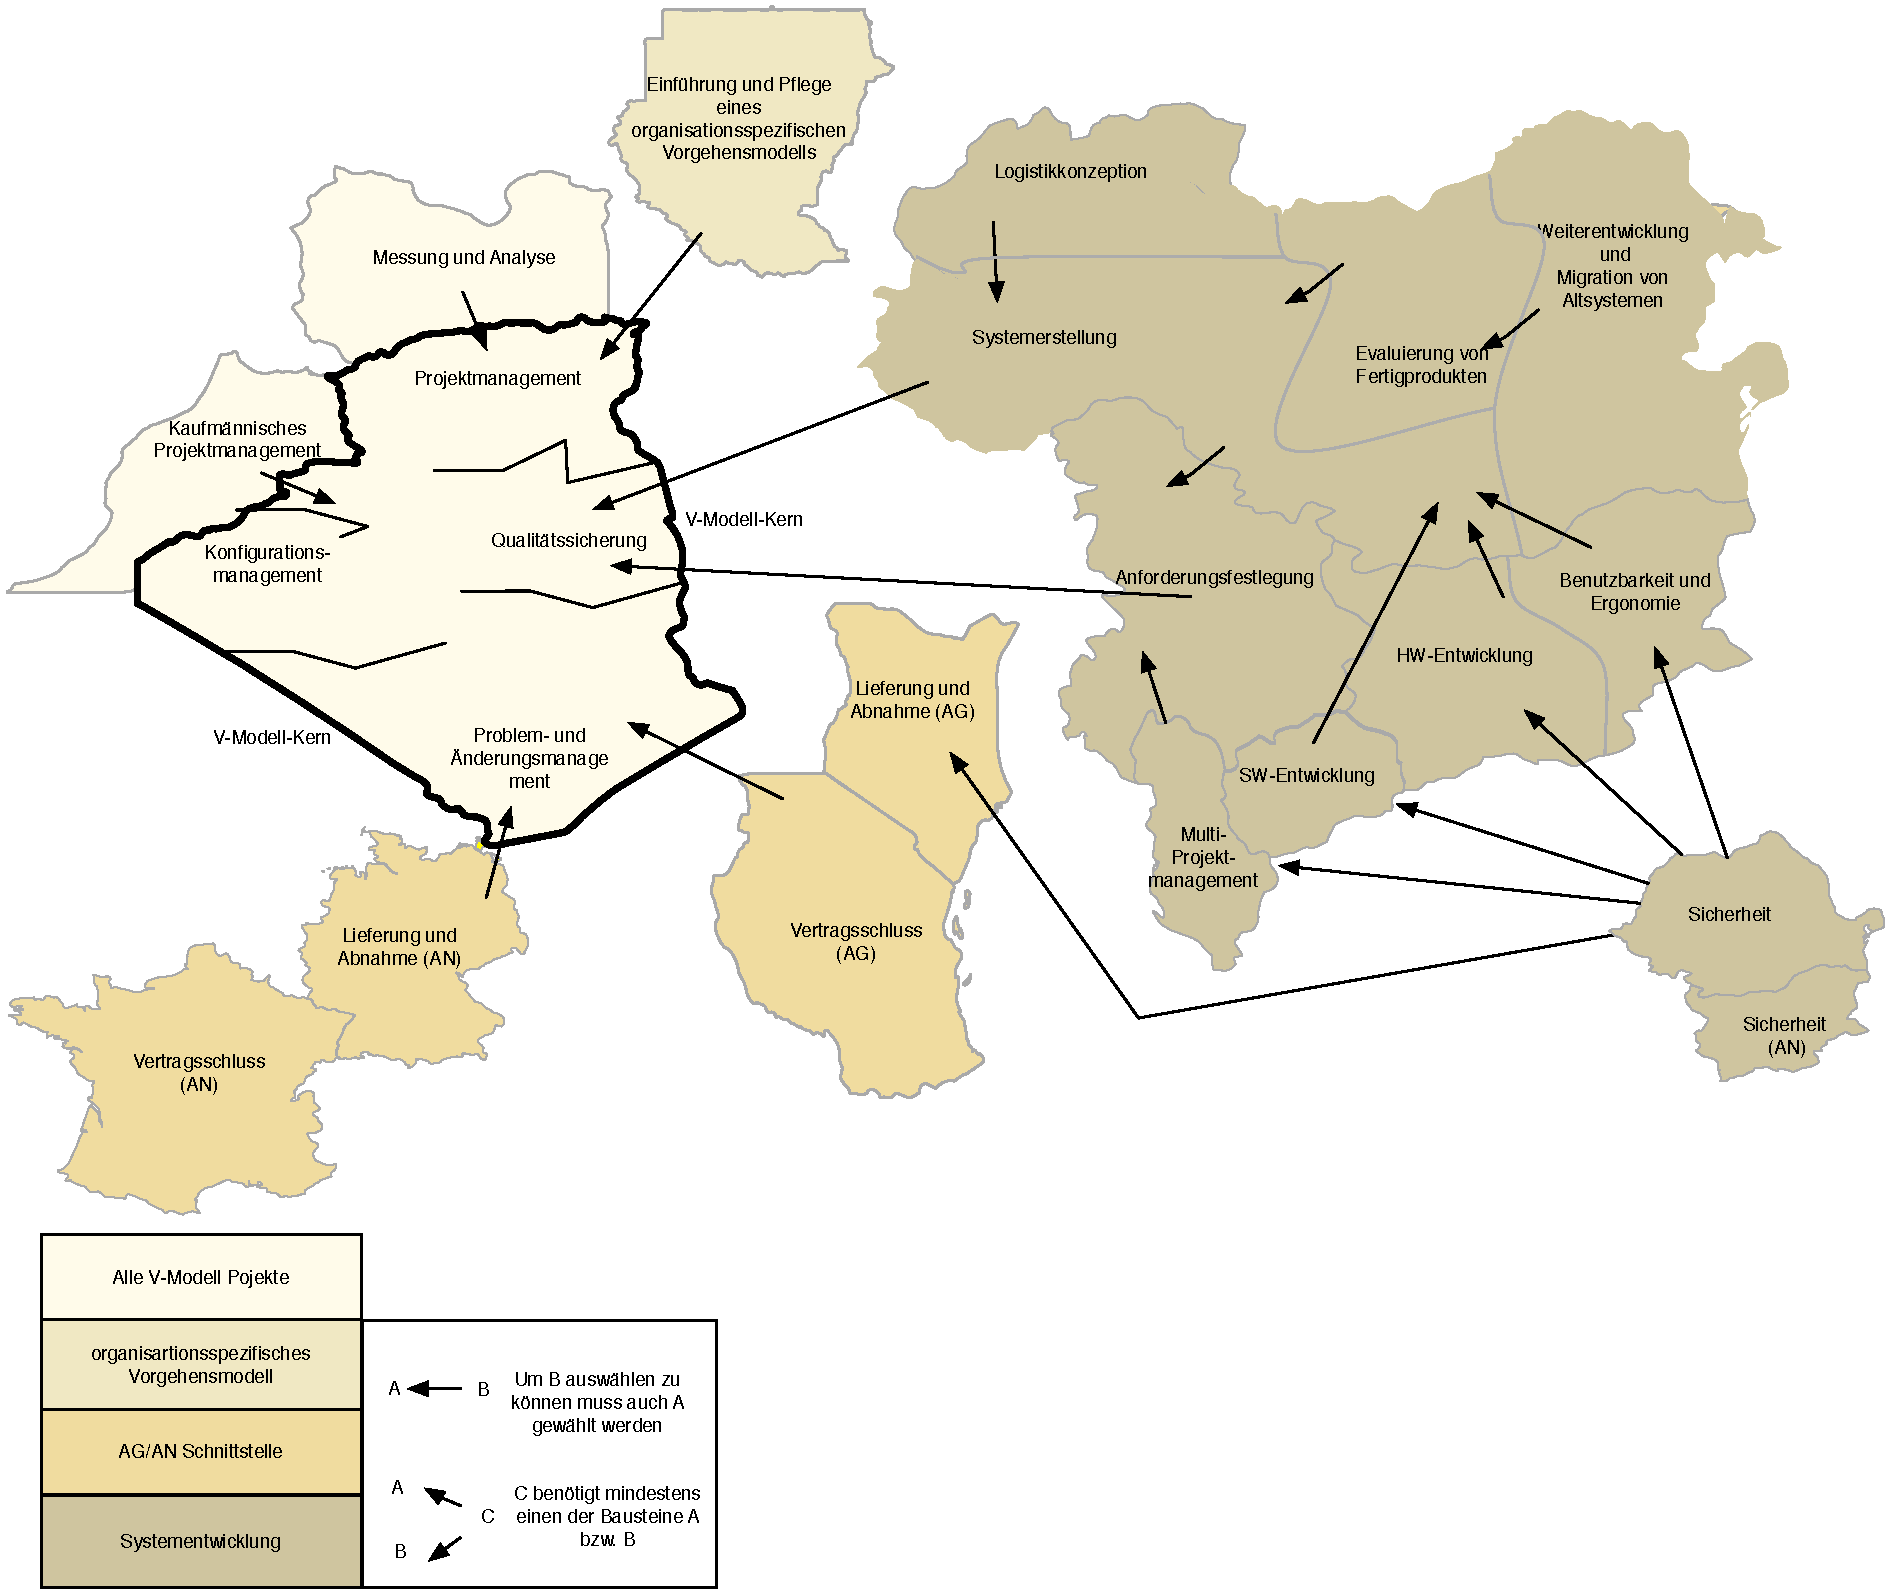
\includegraphics[width=\linewidth]{landkarte} %pdf, jpg, png...
  \caption{V-Modell-Kern und Vorgehensbausteinlandkarte nach \cite{2004vmodell}}
  \label{fig:landkarte}
\end{center}
\end{figure}

 Wie Abbildung \ref{fig:landkarte} zeigt, können die Vorgehensbausteine in die vier Bereiche \textit{Alle V-Modell-Projekte}, \textit{Organisationsspezifisches Vorgehensmodell}, \textit{AG/AN-Schnittstelle} und \textit{Systementwicklung} eingeteilt werden \cite{2004vmodell}.\newline
 Im Bereich \textit{Alle V-Modell-Projekte} finden sich diejenigen Vorgehensbausteine, welche in jedem V-Modell-Projekt herangezogen werden können. Zudem gibt es den V-Modell-Kern, in welchem sich die Vorgehensmodelle finden, die in jedem V-Modell-Projekt unerlässlich sind: \textit{Projektmanagement}, \textit{Konfigurationsmanagement}, \textit{Problem- und Änderungsmanagement} und \textit{Qualitätssicherung}. Zusätzlich zu diesen verpflichtenden Vorgehensbausteinen können in jedem Projekt noch \textit{Kaufmännisches Projektmanagement}, welches bei der Integration des Projektmanagements in das kaufmännische Management hilft und \textit{Messung und Analyse}, welches Verfahren für die organisationsweite und projektübergreifende Erfassung und Auswertung von Kennzahlen bereitstellt, verwendet werden \cite{2004vmodell}.\newline
 Ist der Zweck eines Projektes die Entwicklung eines \textit{Organisationsspezifischen Vorgehensmodells}, so muss der Vorgehensbaustein \textit{Einführung und Pflege eines organisationsspezifischen Vorgehensmodells} hinzugenommen werden. In diesem finden sich Verfahren und Richtlinien für die Einführung eines Vorgehensmodells innerhalb einer Organisation sowie die damit einhergehende Etablierung eines stetigen Verbesserungsprozesses \cite{2004vmodell}.\newline
 Wenn ein Projekt die Entwicklung eines Systems zum Ziel hat, so wird der Bereich \textit{Systementwicklung} herangezogen. In diesem befinden sich die Vorgehensbausteine \textit{Anforderungsfestlegung}, \textit{Systemerstellung}, \textit{HW-Entwicklung}, \textit{SW-Entwicklung}, \textit{Logistikkonzeption}, \textit{Weiterentwicklung und Migration von Altsystemen}, \textit{Evaluierung von Fertigprodukten}, \textit{Benutzbarkeit und Ergonomie}, \textit{Sicherheit} sowie \textit{Sicherheit (AN)} und \textit{Multi-Projektmanagement} \cite{2004vmodell}. \newline
 Im Bereich \textit{AG/AN-Schnittstelle} befinden sich die Vorgehensbausteine für die Kommunikation zwischen Arbeitgeber und Arbeitnehmer: \textit{Lieferung und Abnahme (AG)}, \textit{Lieferung und Abnahme (AN)}, \textit{Vertragsschluss (AG)} und \textit{Vertragsschluss (AN)}. Hier finden sich Regelungen über den Vertrag zwischen Arbeitgeber und Arbeitnehmer sowie über Lieferung und Abnahme des Entwicklungsgegenstandes \cite{2004vmodell}. \newline
 
 \subsubsection{Projektdurchführungsstrategie}
 Die Vorgehensbausteine im V-Modell XT geben zwar an, welche Produkte jeweils zu erstellen und welche Aktivitäten durchzuführen sind, sie geben jedoch hierbei nicht vor, in welcher Reihenfolge dies geschehen soll. Damit das Projekt trotzdem geplant und gesteuert werden kann, gibt es im V-Modell eine Projektdurchführungsstrategie, welche auf den jeweiligen Projekttyp und die Projekttypvariante abgestimmt ist. Hier wird somit die Reihenfolge der Produkte und Aktivitäten festgelegt, also das  \grqq Wann\grqq {} festgelegt. Außerdem werden hier zu erreichende Projektfortschrittsstufen vorgegeben \cite{2004vmodell}. \newline
 
 \subsubsection{Entscheidungspunkte}
Abbildung \ref{fig:entscheidungspunkte} zeigt, dass die in der Projektdurchführungsstrategie vorgegebenen Projektfortschrittsstufen bei Erreichen durch Entscheidungspunkte markiert werden, welche einen Meilenstein im Projektablauf darstellen. Um den Entscheidungspunkt zu erreichen, muss eine vorgegebene Menge an Produkten fertig gestellt werden. Hier entscheidet das Projektmanagement über das Erreichen der Projektfortschrittsstufe und das Freigeben des nächsten Projektabschnitts. Die Entscheidungspunkte, welche im V-Modell XT erreicht werden müssen, können Abbildung \ref{fig:v-modell} entnommen werden. Diese werden wie im V-Modell-Kern in die vier Bereiche \textit{Alle V-Modell-Projekte}, \textit{Organisationsspezifisches Vorgehensmodell}, \textit{AG/AN-Schnittstelle} und \textit{Systementwicklung} unterschieden \cite{2004vmodell}. \newline
Demnach gelten die Entscheidungspunkte \textit{Projekt genehmigt}, \textit{Projekt definiert}, \textit{Iteration geplant} und \textit{Projekt abgeschlossen} für alle Projekttypen und Projektdurchführungsstrategien \cite{2004vmodell}. \newline
Bei der Systementwicklung werden die Entscheidungspunkte \textit{Anforderungen festgelegt}, \textit{System spezifiziert}, \textit{System entworfen}, \textit{Feinentwurf abgeschlossen}, \textit{Systemelemente realisiert} und \textit{System integriert} verwendet. Falls das Projekt vor der Anforderungserhebung in mehrere Teilmodelle aufgeteilt werden soll, werden zusätzlich die Entscheidungspunkte \textit{Gesamtprojekt aufgeteilt} und \textit{Gesamtprojektfortschritt überprüft} hinzugenommen \cite{2004vmodell}. \newline
Die Entscheidungspunkte für die Arbeitgeber/Arbeitnehmer Schnittstelle setzen sich aus \textit{Projekt ausgeschrieben}, \textit{Angebot abgegeben}, \textit{Projekt beauftragt}, \textit{Lieferung durchgeführt}, \textit{Abnahme erfolgt} und \textit{Projektfortschritt überprüft} zusammen \cite{2004vmodell}. \newline
 Bei der Entwicklung eines organisationsspezifischen Vorgehensmodells kommen die Entscheidungspunkte \textit{Vorgehensmodell analysiert}, \textit{Verbesserung Vorgehensmodell konzipiert} und \textit{Verbesserung Vorgehensmodell realisiert} zum Einsatz \cite{2004vmodell}. \newline
 Die Entscheidungspunkte legen das \grqq Wann\grqq {} und \grqq Was\grqq {} fest, d.h. wann welche Produkte fertig gestellt sein müssen.

 
 
 \begin{figure}[!htbp]
\begin{center}
  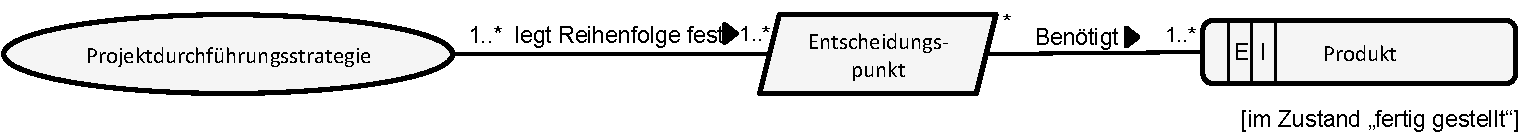
\includegraphics[width=\linewidth]{Entscheidungspunkte} %pdf, jpg, png...
  \caption{Entscheidungspunkte V-Modell XT nach \cite{2004vmodell}}
  \label{fig:entscheidungspunkte}
\end{center}
\end{figure}
 
\begin{sidewaysfigure}[!htbp]
\begin{center}
  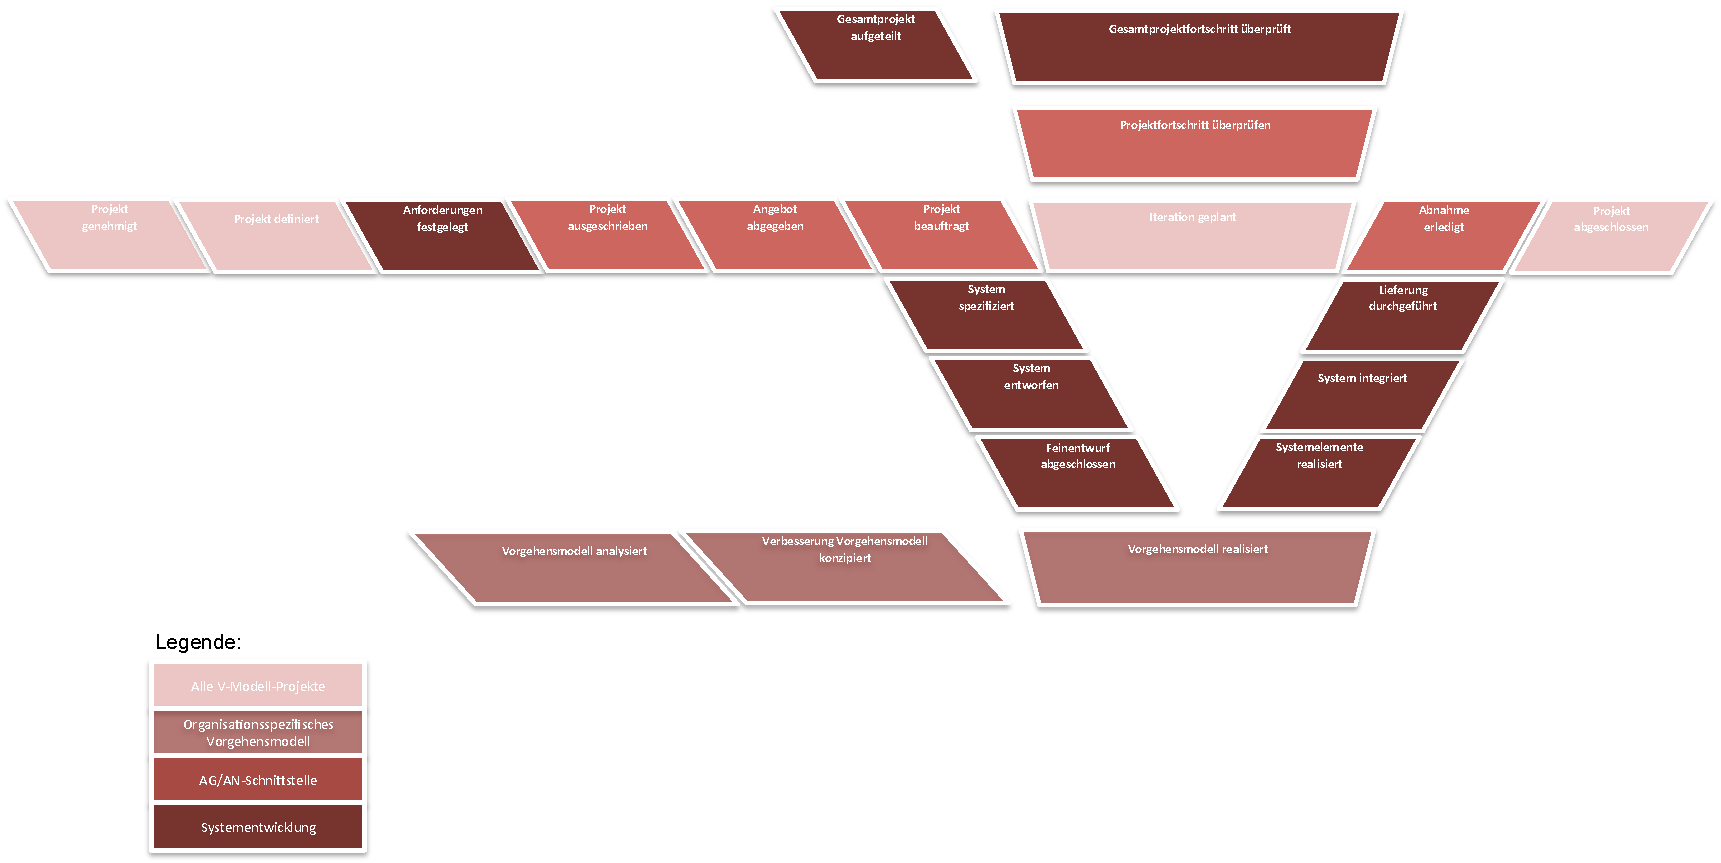
\includegraphics[width=\linewidth]{v-modell} %pdf, jpg, png...
  \caption{Entscheidungspunkte für die Projektdurchführungsstrategie nach \cite{2004vmodell}}
  \label{fig:v-modell}
\end{center}
\end{sidewaysfigure}

Im Folgenden werden Teile des V-Modells XT modelliert, da das ganze V-Modell in dieser Arbeit nicht  modelliert werden kann. Aus diesem Grund wird zum Einen das \textit{Systementwicklungsprojekt AG/AN} modelliert. Weiterhin wird ein hierzu gehöriger Unterprozess \textit{Inkrementelle Entwicklung} und die hierzu gehörenden Unterprozesse \textit{System entwerfen} und \textit{System spezifizieren} modelliert.
\clearpage

\subsection{Imperative Modellierung V-Modell}



\subsubsection{Systementwicklungsprojekt AG/AN}


Die imperative Modellierung von \textit{Systementwicklungsprojekt AG/AN}  zeigt Abbildung \ref{fig:Systementwicklung}. \newline
Zunächst muss ein Projekt genehmigt und definiert werden. Dies ist durch die einander folgenden Aktivitäten\textit{Projekt genehmigen} und \textit{Projekt definieren} dargestellt.\newline
In der nachfolgenden Aktivität müssen sodann die \textit{Anforderungen festgelegt werden}, bevor die \textit{Iteration geplant} werden kann. \newline
Hiernach muss entschieden werden, ob eine \textit{Prototypische Entwicklung durchgeführt}, eine \textit{Komponentenbasierte Entwicklung durchgeführt} oder eine \textit{Inkrementelle Entwicklung durchgeführt} werden soll. Dies wird durch das XOR-Gateway beschrieben, welche nur eine Alternative zulässt.\newline
Anschließend wird das \textit{System abgenommen}.\newline
An dieser Stelle wird entschieden, ob erneut zu \textit{Anforderungen festlegen} zurückgekehrt wird und der Prozess ab dieser Aktivität erneut startet oder ob zu \textit{Projekt ausschreiben} zurückgekehrt wird und der Prozess ab hier erneut startet. Ansonsten endet der Prozess mit der Aktivität \textit{Projekt abschließen}.

\begin{figure}[!htbp]
\begin{center}
  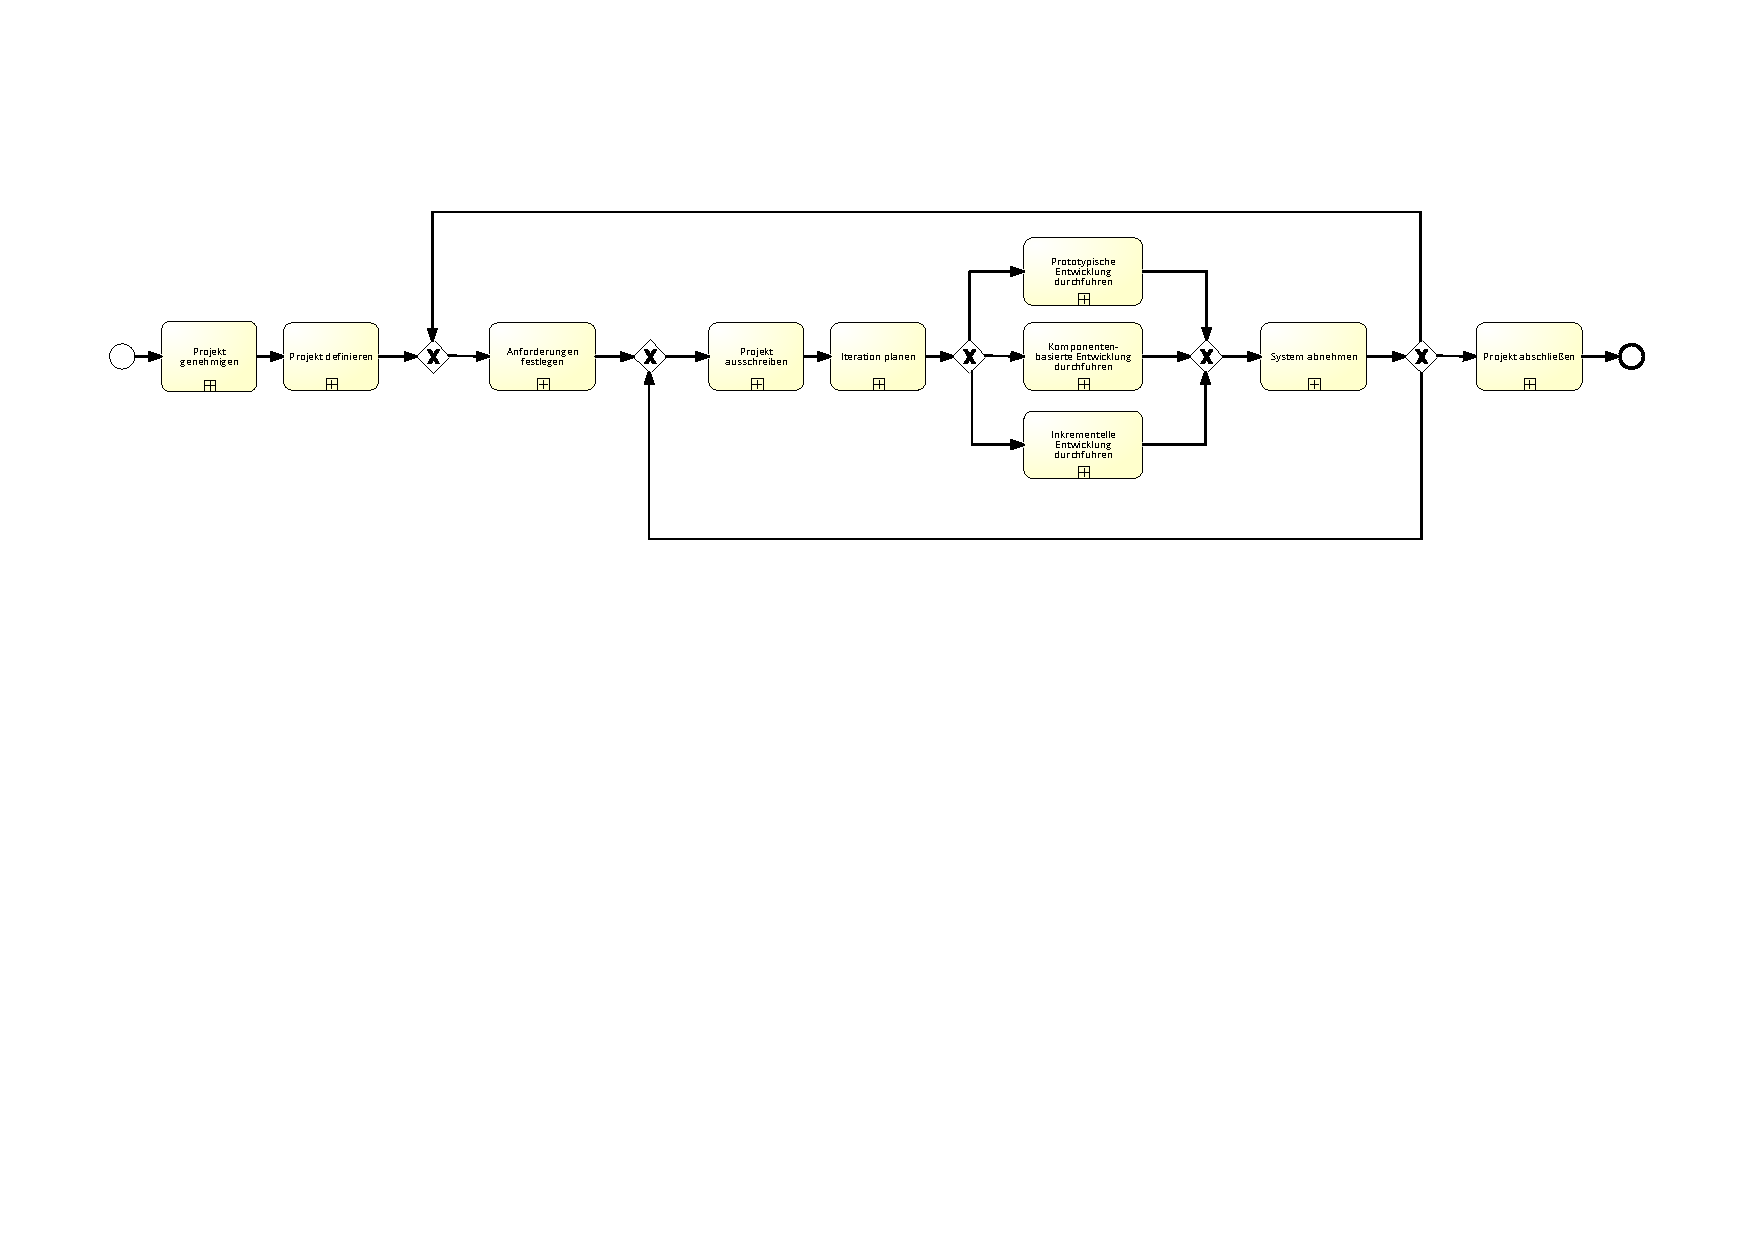
\includegraphics[width=\linewidth]{Systementwicklungimp} %pdf, jpg, png...
  \caption{Systementwicklungsprojekt AG/AN  V-Modell - imperativ}
  \label{fig:Systementwicklungimp}
\end{center}
\end{figure}




\subsubsection{Inkrementelle Entwicklung durchführen}
In Abbildung \ref{fig:Inkrementell} ist die imperative Modellierung des Unterprozesses \textit{Inkrementelle Entwicklung durchführen} abgebildet. \newline
Zu Beginn muss das \textit{System spezifiziert} werden und anschließend wird das \textit{System entworfen}. \newline
Hiernach wird der \textit{Feinentwurf entworfen} und es werden die \textit{Systemelemente realisiert}. Diese beiden Aktivitäten können so oft wie nötig durchgeführt werden, was durch das XOR-Gateway beschrieben ist.  \newline
Im nächsten Schritt wird das \textit{System integriert} und es beginnt eine neue Iteration bei der Aktivität System entwerfen.\newline
Falls keine weitere Iteration mehr notwedig ist, wird die \textit{Lieferung durchgeführt} und der Unterprozess endet hier. \newline

\begin{figure}[!htbp]
\begin{center}
  \includegraphics[width=\linewidth]{Inkrementell} %pdf, jpg, png...
  \caption{Unterprozess Inkrementelle Entwicklung durchführen V-Modell - imperativ}
  \label{fig:Inkrementell}
\end{center}
\end{figure}



\clearpage


\subsubsection{System entwerfen}

Abbildung \ref{fig:SystementwurfKlein} zeigt die imperative Modellierung des Unterprozesses \textit{System entwerfen}.\newline
Die Aktivitäten \textit{Systemarchitektur erstellen, Unterstütungssystemarchitektur erstellen, Styleguide für die Mensch-Maschine-Schnittstelle erstellen, HW-Architektur erstellen, SW-Architektur erstellen, Datenbankentwurf erstellen, Implementierungs-, Integrations- und Prüfkonzept Unterstützungssystem erstellen, Integrations- und Prüfkonzept Hardware (HW) erstellen, Integrations- und Prüfkonzept Software (SW) erstellen} und \textit{Migrationskonzept erstellen} werden hier nacheinander ausgeführt.
\begin{figure}[!htbp]
\begin{center}
  \includegraphics[width=\linewidth]{SystementwurfKlein} %pdf, jpg, png...
  \caption{System entwerfen V-Modell - imperativ}
  \label{fig:SystementwurfKlein}
\end{center}
\end{figure}


\subsubsection{System spezifizieren}


Am Anfang des Unterprozesses \textit{System spezifizieren} (Abbildung \ref{fig:BerichtswesenimpKlein}) muss eine \textit{Besprechung durchgeführt} werden. Hieraus entsteht das Artefakt \textit{Besprechungsdokument}.\newline
Parallel zu allen anderen Aktivitäten ist bei Bedarf bei jeder Änderung das \textit{Projekttagebuch zu führen}. Dies wird durch das Parallel-Gateway sichergstellt und die XOR-Schleife stellt sicher, dass die Akrtivität so oft durchgeführt wird, wie Anpassungen notwendig sind. \newline
Im nächsten Schritt werden die \textit{Messdaten erfasst}.\newline
In der nachfolgenden Aktivität wird die \textit{Metrik berechnet und ausgewertet}, woraus das Artefakt \textit{Metrikauswertung} entsteht.\newline
Anschließend erfolgt die Durchführung der Aktivität \textit{Kaufmännischen Projektstausbericht erstellen}, wobei das Artefakt \textit{Kaufmännischer Projektstausbericht} als Artefakt herauskommt.\newline
Bei der nächsten Aktivität wird der \textit{Prjektstatusbericht erstellt} und danach wird der \textit{Gesamtprojektfortschritt erittelt}\newline
Die Aktivität \textit{QS-Bericht erstellen} bringt dann das Artefakt \textit{QS-Bericht hervor} und die nachfolgende Aktivität \textit{Projekt abschließen} den \textit{Projektabschlußbericht}.

\begin{figure}[!htbp]
\begin{center}
  \includegraphics[width=\linewidth]{BerichtswesenimpKlein} %pdf, jpg, png...
  \caption{System spezifizieren-imperativ}
  \label{fig:BerichtswesenimpKlein}Anzahl unterschiedliche Gateways/Constraints\end{center}
\end{figure}

\clearpage
\subsection{Deklarative Modellierung V-Modell}


Die deklarative Modellierung von \textit{Systementwicklungsprojekt AG/AN}  zeigt Abbildung \ref{fig:SystemV}. \newline
Zunächst muss ein Projekt genehmigt und definiert werden. Dies ist durch die aufeinander folgenden Aktivitäten \textit{Projekt genehmigen} und \textit{Projekt definieren} dargestellt, welche durch das Constraint \textit{succession} verbunden sind.\newline
In der nachfolgenden Aktivität müssen sodann die \textit{Anforderungen festgelegt werden}, bevor die \textit{Iteration geplant} werden kann. \newline
Hiernach muss entschieden werden, ob eine \textit{Prototypische Entwicklung durchgeführt}, eine \textit{Komponentenbasierte Entwicklung durchgeführt} oder eine \textit{Inkrementelle Entwicklung durchgeführt} werden soll. Dies wird hier durch einen extra Unterprozess \textit{Entwicklung durchführen} (Abbildung \ref{fig:SystemVUnter} dargestellt, da dieser Sachverhalt auf Grund der Schleifen im Prozess ohne Unterprozess nicht darstellbar war. Im Unterprozess kann dann eine der drei Aktivitäten ausgeführt werden, was das Constraint \textit{1of 3} vorgibt.\newline
Anschließend wird das \textit{System abgenommen}.\newline
An dieser Stelle wird enschieden, ob erneut zu \textit{Anforderungen festlegen} zurückgekehrt wird und der Prozess ab dieser Aktivität erneut startet oder ob zu \textit{Projekt ausschreiben} zurückgekehrt wird und der Prozess ab hier erneut startet. Ansonsten endet der Prozess mit der Aktivität \textit{Projekt abschließen}.

\begin{figure}[!htbp]
\begin{center}
  \includegraphics[width=\linewidth]{SystemV} %pdf, jpg, png...
  \caption{Systementwicklungsprojekt AG/AN  V-Modell - deklarativ}
  \label{fig:SystemV}
\end{center}
\end{figure}

\begin{figure}[!htbp]
\begin{center}
  \includegraphics[width=\linewidth]{SystemVUnter} %pdf, jpg, png...
  \caption{Systementwicklungsprojekt AG/AN  V-Modell Unterprozess Entwicklung durchführen - deklarativ}
  \label{fig:SystemVUnter}
\end{center}
\end{figure}



\subsubsection{Inkrementelle Entwicklung durchführen}
In Abbildung \ref{fig:Systementwicklung} ist die deklarative Modellierung des Unterprozesses \textit{Inkrementelle Entwicklung durchführen} abgebildet. \newline
Zu Beginn muss das \textit{System spezifiziert} werden, weshalb diese Aktivität mit dem Constraint \textit{init} beschrieben ist und anschließend wird das \textit{System entworfen}, was durch das Constraint \textit{succession} zwischen diesen beiden Aktivitäten sichergestellt wird.\newline
Hiernach wird der Feinentwurf entworfen und Systemelemente realisiert. Diese beiden Aktivitäten können so oft wie nötig durchgeführt werden. Es kommt nur darauf an, dass zuerst die Aktivität  \textit{Feinentwurf entwerfen} und anschließend die Aktivität \textit{Systemelemente realisieren} durchgeführt wird, weshalb das Constraint \textit{chain succession} sich zwischen diesen beiden Aktivitäten befindet. \newline
Im nächsten Schritt wird das System integriert und es beginnt eine neue Iteration bei der Aktivität System entwerfen. Aus diesem Grund befindet sich hier das Constraint \textit{alternate succession} zwischen den Aktivitäten \textit{System integrieren} und \textit{System entwerfen}, da eine erneute Ausführung von \textit{System entwerfen} erst nach Ausführung der Aktivität \textit{System integrieren} möglich ist. \newline
Falls keine weitere Iteration mehr notwendig ist, wird die \textit{Lieferung durchgeführt} und der Unterprozess endet hier, da durch die Constraints zu \textit{System entwerfen} und \textit{Feinentwurf entwerfen} keine weitere Aktivität mehr ausgeführt werden kann. \newline
\begin{figure}[!htbp]
\begin{center}
  \includegraphics[width=\linewidth]{Systementwicklung} %pdf, jpg, png...
  \caption{Unterprozess Inkrementelle Entwicklung durchführen V-Modell - imperativ}
  \label{fig:Systementwicklung}
\end{center}
\end{figure}



\subsubsection{System entwerfen}


Abbildung \ref{fig:SystementwurfKleinDec} zeigt die deklarative Modellierung von System entwerfen.\newline
Die Aktivitäten \textit{Systemarchitektur erstellen, Unterstütungssystemarchitektur erstellen, Styleguide für die Mensch-Maschine-Schnittstelle erstellen, HW-Architektur erstellen, SW-Architektur erstellen, Datenbankentwurf erstellen, Implementierungs-, Integrations- und Prüfkonzept Unterstützungssystem erstellen, Integrations- und Prüfkonzept Hardware (HW) erstellen, Integrations- und Prüfkonzept Software (SW) erstellen} und \textit{Migrationskonzept erstellen} werden hier nacheinander ausgeführt. Da die vorherige Aktivität immer Voraussetzung für das Ausführen der nachfolgenden Aktivität ist, und die nachfolgende Aktivität nach der vorherigen ausgeführt werden muss, ist zwischen allen Aktivitäten jeweils \textit{succession} als Constraint eingefügt.

\begin{figure}[!htbp]
\begin{center}
  \includegraphics[width=\linewidth]{SystementwurfKleinDec} %pdf, jpg, png...
  \caption{System entwerfen - deklarativ}
  \label{fig:SystementwurfKleinDec}
\end{center}
\end{figure}

\subsubsection{System spezifizieren}


Am Anfang von System spezifizieren (Abbildung \ref{fig:BerichtswesenKlein}) muss eine \textit{Besprechung durchgeführt} werden. Dies wird durch das Constraint \textit{init} sichergestellt.\newline
Bei jeder Änderung muss die Aktivität \textit{Projekttagebuch fuehren} ausgeführt werden. Aus diesem Grund ist diese durch kein Constraint mit einer anderen Aktivität verbunden, da sie jederzeit ausgeführt werden kann und so oft wie nötig.\newline
Im nächsten Schritt werden die \textit{Messdaten erfasst}. Da ab hier alle Aktivitäten nacheinander auszuführen sind, sind dies jeweils durch das Constraint \textit{succession} verbunden.\newline
In der nachfolgenden Aktivität wird die \textit{Metrik berechnet und ausgewertet}.\newline
Anschließend erfolgt die Durchführung der Aktivität \textit{Kaufmännischen Projektstatusbericht erstellen}\newline
Bei der nächsten Aktivität wird der \textit{Prjektstatusbericht erstellt} und danach wird der \textit{Gesamtprojektfortschritt erittelt}\newline
Danach werden noch die Aktivitäten \textit{QS-Bericht erstellen}und \textit{Projekt abschließen} ausgeführt.

\begin{figure}[!htbp]
\begin{center}
  \includegraphics[width=\linewidth]{BerichtswesenKlein} %pdf, jpg, png...
  \caption{System spezifizieren- deklarativ}
  \label{fig:BerichtswesenKlein}
\end{center}
\end{figure}

\clearpage

\subsection{Vergleich}


Abbildung \ref{fig:SystementwicklungsprojektExcel} zeigt die Zahl notwendigen Elemente zur Darstellung des Prozesses Systementwicklungsprojekt AG/AN. In ConDec (11 Aktivitäten)  ist somit einer Aktivität mehr zur Darstellung nötig als in BPMN (10 Aktivitäten). In BPMN werden vier Gateways und 20 Sequenzflusselemente verwendet. In ConDec hingegen braucht es 11 Constraints. In ConDec werden sieben unterschiedliche Constraints im Modell verwendet, in BPMN eines. Somit sind zur Darstellung des Sachverhaltes insgesamt 34 BPMN Elemente 25 ConDec Elemente notwendig.\newline

\begin{figure}[!htbp]
\begin{center}
  \includegraphics[scale=0.6]{SystementwicklungsprojektExcel} %pdf, jpg, png...
  \caption{Systementwicklungsprojekt AG/AN}
  \label{fig:SystementwicklungsprojektExcel}
\end{center}
\end{figure}

Die Anzahl der Elemente zur Darstellung des Prozesses Inkrementelle Entwicklung kann Abbildung \ref{fig:InkrementellExcel} entnommen werden. Es werden jeweils sechs Aktivitäten verwendet. Weiterhin werden in BPMN vier Gateways und 13 Sequenzflüsse zur Darstellung des Prozessablaufes benötigt. In ConDec sind hierfür neun Constraints und zwei Existenz-Constraints notwendig. BPMN benötigt ein Gateway, also keine verschiedenen Gateways und ConDec braucht sechs unterschiedliche Constraints. Somit ergeben sich in Summe 23 BPMN Elemente und 17 ConDec Elemente zur Darstellung des Sachverhaltes. \newline

\begin{figure}[!htbp]
\begin{center}
  \includegraphics[scale=0.6]{InkrementellExcel} %pdf, jpg, png...
  \caption{Inkrementelle Entwicklung}
  \label{fig:InkrementellExcel}
\end{center}
\end{figure}

Abbildung \ref{fig:SystementwurfExcel} zeigt die Anzahl der Elemente, welche zur Darstellung des Prozesses System entwerfen notwendig sind. Demnach werden in beiden Prozessmodellierungssprachen jeweils 11 Aktivitäten verwendet. In BPMN werden keine Gateways und 12 Sequenzflusselemente benötigt. ConDec braucht zur Darstellung des Sachverhaltes 10 Constraints und 11 Existenz-Constraints, jedoch keine unterschiedlichen Constraints. In Summe sind somit in BPMN 23 Elemente und in ConDec 32 Elemente zur Darstellung notwendig.\newline

\begin{figure}[!htbp]
\begin{center}
  \includegraphics[scale=0.6]{SystementwurfExcel} %pdf, jpg, png...
  \caption{System entwerfen}
  \label{fig:SystementwurfExcel}
\end{center}
\end{figure}

In Abbildung \ref{fig:SpezifizierenExcel} ist die Anzahl der Elemente zur Darstellung des Prozesses System spezifizieren abgetragen. Demnach werden neun Aktivitäten verwendet sowohl in BPMN als auch in ConDec. Es werden drei Gateways und 15 Sequenzflüsse in BPMN benötigt. In ConDec werden acht Constraints und neun Existenz-Constraints zur Darstellung verwendet. Weiterhin gibt es zwei unterschiedliche Gateways in BPMN und zwei unterschiedliche Constraints in ConDec. Insgesamt ergeben sich somit 27 unterschiedliche Elemente in BPMN und 26 unterschiedliche Elemente in ConDec. \newline

\begin{figure}[!htbp]
\begin{center}
  \includegraphics[scale=0.6]{SpezifizierenExcel} %pdf, jpg, png...
  \caption{System spezifizieren}
  \label{fig:SpezifizierenExcel}
\end{center}
\end{figure}

Die semantische \textit{Richtigkeit} kann von ConDec in Bezug auf die Darstellung von Rollen und Artefakten nicht eingehalten werden. Hier werden Grenzen der Darstellbarkeit in ConDec erreicht.\newline
Sowohl BPMN, als auch ConDec können die syntaktische \textit{Richtigkeit} jedoch einhalten, da in beiden Modellierungssprachen die Notationsregeln bei der Modellierung der Prozessmodelle eingehalten werden können.\newline
 
Der  Grundsatz des \textit{systematischen Aufbaus} kann bei ConDec wiederum nicht eingehalten werden, da keine Artefakte modelliert werden können.\newline

Der Grundsatz der \textit{Relevanz} kann wieder von beiden Prozessmodellierungssprachen eingehalten werden, da sich sowohl die ConDec-Modelle, als auch die BPMN-Modelle mit den minimal relevanten Informationen erstellen lassen.\newline

Der Grundsatz der \textit{Wirtschaftlichkeit} kann wiederum bei beiden Prozessmodellierungssprachen eingehalten werden, da sich der Aufwand zur Erstellung der Prozessmodelle nicht voneinander unterscheidet. 


Beim Grungsatz der \textit{Klarheit} gibt es Unterschiede zwischen den Modellen. Zur Darstellung der beiden Prozesse Systementwicklungsprojekt AG/AN und Inkrementelle Entwicklung werden in ConDec jeweils viele unterschiedliche Constraints benötigt (acht bei Systementwicklungsprojekt AG/AN und sechs bei Inkrementelle Entwicklung). Dies wirkt sich sehr negativ auf die Verständlichkeit aus, da sechs bis acht unterschiedliche, teilweise sehr komplexe Constraints verstanden werden müssen. Auch wenn BPMN bei diesen Modellen eine höhere Anzahl an Elementen insgesamt aufweist, weisen die beiden ConDec-Modelle eine höhere Komplexität auf, weswegen die BPMN-Modelle verständlicher sind. \newline
Beim Prozess Systementwurf hingegen, weist ConDec  insgesamt eine höhere Anzahl an Elementen auf. Weiterhin werden hier bei ConDec 10 Constraints verwendet, in BPMN hingegen keine Gateways. Aus diesem Grund ist hier das mit BPMN erstellete Modell das weniger komplexe und somit auch das verständlichere.\newline
Beim Prozess System spezifizieren werden in BPMN drei Gateways verwendet und in ConDec acht Constraints. Bei beiden handelt es sich hierbei um zwei unterschiedliche Gateways/Constraints. Da ConDec hier eine höhere Anzahl an Constraints aufweist, als BPMN Gateways, ist das mit BPMN erstellte Modell hier das verständlichere. \newline
Somit lässt sich insgesamt hier festhalten, das beim Grundsatz der \textit{Klarheit} BPMN hier die geeignetere Modellierungssprache ist, da sie hier weniger komplexe Modelle erzeugt.\newline

Bei Ausführung der Prozesse in den Modellierungstools Signavio und Declare weiden beide das gleiche Ausführungsverhalten auf, wodurch hier die \textit{Vergleichbarkeit} gewährleistet ist. \newline
Die Anzahl der Elemente in den Prozessmodellen unterscheidet sich teilweise. Bei BPMN werden bei den Prozessen Systementwicklungsprojekt AG/AN deutlich mehr Elemente zur Darstellung des gleichen Sachverhaltes verwendet wie bei ConDec. Beim Prozess Systementwurf werden bei ConDec mehr Elemente benötigt, wie bei BPMN und bei System spezifizieren werden in etwa gleich viele Elemente verwendet.\newline
Die \textit{Vergleichbarkeit} kann jedoch in Bezug auf Artefakte und Rollen, außer bei den Phasen des Open UP (hier werden noch keine Artefkate und Rollen verwendet) nicht eingehalten werden.\newline
Somit weisen bei der \textit{Vergleichbarkeit} beide Prozessmodellierungssprachen Stärken und Schwächen auf. \newline
Abbildung \ref{fig:TabelleVModell} gibt nochmal eine zusammenfassende Übersicht über die Ergebniss des Vergleichs. 


\begin{figure}[!htbp]
\begin{center}
  \includegraphics[scale=0.6]{TabelleVModell} %pdf, jpg, png...
  \caption{Übersicht Vergleich V-Modell}
  \label{fig:TabelleVModell}
\end{center}
\end{figure}




\section{Fazit}

Prozesse viele Aktivitäten parallel=>ConDec besser, da weniger unterschiedliche Verbindungselemente
Prozesse viele XOR => BPMN besser, da weniger unterschiedliche Verbindungselemente bei kleinen weniger, bei großen(>5 Aktivitten) viel mehr
keine Verzweigungen/Parallel=>beide gleich


Bei fehlen ConDec wichtige Informationen wie z.B. Rollen/Dokumente die zum Verständnis des gesamten Prozesses wichtig sind, wan welche verzweigung genommen wird 





